\documentclass[11pt]{article}
\usepackage[a4paper,margin=2.6cm,headheight=14pt]{geometry}
\usepackage[T1]{fontenc}
\usepackage{lmodern}
\usepackage{microtype}
\usepackage{amsmath,amssymb,amsthm,mathtools}
\usepackage{booktabs,tabularx,longtable,array}
\usepackage{enumitem}
\usepackage{xcolor}
\usepackage{listings}
\usepackage{fancyhdr}
\usepackage{tikz}
\usetikzlibrary{positioning}
\usepackage{caption}
\usepackage[hidelinks]{hyperref}
\usepackage[capitalise,nameinlink]{cleveref}

\definecolor{dcblue}{RGB}{28,58,92}
\definecolor{dcgray}{RGB}{246,246,246}
\definecolor{dcrule}{RGB}{190,190,190}

\hypersetup{colorlinks=true,linkcolor=dcblue,citecolor=dcblue,urlcolor=dcblue}
\hypersetup{pdftitle={MeTTaDinC: An Executable Language for Observer-Relative Abstraction, Evidence, and Composition},
  pdfsubject={Specification draft, 4 November 2026},
  pdfkeywords={MeTTaDinC, distinction calculus, abstraction, certificates, Hyperon}}

\lstdefinestyle{metta}{
  basicstyle=\ttfamily\small,
  backgroundcolor=\color{dcgray},
  frame=single, rulecolor=\color{dcrule}, framesep=4pt,
  columns=fullflexible, keepspaces=true,
  showstringspaces=false, breaklines=true,
  aboveskip=8pt, belowskip=8pt, xleftmargin=2pt, xrightmargin=2pt
}
\lstset{style=metta}

\newcommand{\code}[1]{\texttt{#1}}
\newcommand{\ab}{\bar\alpha}
\newcommand{\lift}{^{\sharp}}
\newcommand{\br}[2]{\langle #1 \mid #2 \rangle}
\newcommand{\Lt}{\otimes}
\newcommand{\gfp}{\operatorname{gfp}}
\newcommand{\TV}{\operatorname{TV}}
\newcommand{\Hom}{\operatorname{Hom}}
\newcommand{\End}{\operatorname{End}}
\newcommand{\rank}{\operatorname{rank}}
\newcommand{\dom}{\operatorname{dom}}
\newcommand{\Poly}{\mathbf{Poly}}
\newcommand{\Q}{\mathbb{Q}}
\newcommand{\F}{\mathbb{F}}
\newcommand{\dnow}{\delta_{\mathrm{now}}}
\newcommand{\dupd}{\delta_{\mathrm{upd}}}
\newcommand{\dbd}{\delta_{\mathrm{beh}}}
\newcommand{\dtr}{\delta_{\mathrm{tr}}}
\newcommand{\abeh}{\alpha_{\mathrm{beh}}}
\newcommand{\dbeh}{d_{\mathrm{beh}}}
\newcommand{\Pbeh}{P_{\mathrm{beh}}}
\newcommand{\plain}{\paragraph{In plain terms.}}

\theoremstyle{definition}
\newtheorem{definition}{Definition}[section]
\newtheorem{example}[definition]{Example}
\newtheorem{remark}[definition]{Remark}
\theoremstyle{plain}
\newtheorem{proposition}[definition]{Proposition}
\newtheorem{theorem}[definition]{Theorem}
\newtheorem{lemma}[definition]{Lemma}
\newtheorem{corollary}[definition]{Corollary}

\setlist{itemsep=2pt,topsep=4pt}
\setlength{\parskip}{3pt}
\setlength{\emergencystretch}{2.5em}

\pagestyle{fancy}
\fancyhf{}
\fancyhead[L]{\small MeTTaDinC}
\fancyhead[R]{\small Specification draft, 4 November 2026}
\fancyfoot[C]{\small\thepage}
\renewcommand{\headrulewidth}{0.4pt}

\begin{document}

\hypersetup{pageanchor=false}
\begin{titlepage}
\thispagestyle{empty}
\vspace*{2.2cm}
{\color{dcblue}\large\scshape Language design and research specification\par}
\vspace{1.4cm}
{\color{dcblue}\fontsize{30}{36}\selectfont\bfseries MeTTaDinC\par}
\vspace{0.6cm}
{\LARGE\bfseries An Executable Language for\\[2pt] Observer-Relative Abstraction,\\[2pt] Evidence, and Composition\par}
\vspace{0.7cm}
{\large Graded distinctions, typed claims, symbolic carriers,\\ hives, and six application laboratories\par}
\vspace{1.6cm}
{\large Specification draft\par}
{4 November 2026\par}
\vspace{0.8cm}
{Developed from the d-calculus and Hyperseed project\par}
\vfill
\noindent\begin{minipage}{\textwidth}
\small
{\color{dcblue}\bfseries Scope.} A proposed MeTTa sublanguage whose core is graded: every
adequacy question can be measured as a defect or checked against a bound, and the crisp yes/no
answers are the special case of a two-valued algebra. Deterministic, stochastic and
nondeterministic dynamics; enumerated, symbolic and space-backed carriers; quotient, graded,
simulation, linear and transfer arrows, each with its own registered composition law; typed
claims that say which notion of sameness was established; replayable evidence throughout. Cetta
is the proposed first host.

\smallskip
{\color{dcblue}\bfseries Validation package.} A machine-readable registry of declarations and
requests, complete fixture modules for every example, a claims manifest, an exact-arithmetic
oracle with its results, a static checker that ties these together, and pinned tool versions.
The listings in this document are excerpts of those fixtures, and the registry and fixtures are
authoritative where the text and they differ. A coding-agent implementation guide of the same date
accompanies this specification. No MeTTaDinC runtime exists yet.
\end{minipage}
\end{titlepage}
\hypersetup{pageanchor=true}

\begin{abstract}
\noindent
An intelligent system keeps some distinctions and discards others, and whether a discarded
distinction mattered depends on what the system will later ask and do. MeTTaDinC is a proposed
MeTTa sublanguage that makes this dependence explicit and executable. A program declares
carriers, observers, operations and candidate encodings; the language measures how much each
encoding loses, explains the loss with replayable witnesses, repairs it, induces abstract
operations, and composes the results. Observers are tolerances in the sense of the distinction
calculus, so current adequacy, compatibility of encoded updates and behavioral adequacy are
inequalities between tolerances, and each can be measured as a defect or checked against a
bound. The behavioral tolerance is a greatest fixed point whose complement is the bisimulation
pseudometric; for two-valued tolerances computing it is ordinary partition refinement.

Several different answers to the question ``what may be forgotten?'' are legitimate, and the
language keeps them apart as typed claims: literal equality and equality up to a declared
observer; bisimulation, trace equivalence and quantitative trace discrepancy; simulation for
sound over-approximation; exact and approximate induction of abstract machines; signed and
positive linear realizations. A seven-state stochastic chain, a mandatory fixture, shows three of
these answers disagreeing on the same states. Each arrow kind has its own composition law,
including a norm-aware law for signed linear arrows, and hives come in two typed forms: kernel
hives governed by metric coherence and transfer hives governed by response preservation up to a
declared gauge. Carriers may be enumerated, symbolic or drawn from a pinned space snapshot; the
symbolic path has an explicit admission contract, and a forty-bit fixture with eight behavioral
classes, together with an adversarial candidate that covers only four of its words, keeps that
contract in the first acceptance target.

Hyperseed supplies the main ontology application, and six laboratories cover neural report
audits, evolutionary archives, skill-transfer hives, regime repair, arithmetic observer
discovery, and over-approximation of an access protocol. The final sections connect the design to
finite OmegaPLN, MeTTaProN, $\omega$PLN and MORK, and to the inspected source of Cetta at a
pinned revision. The contribution is an integrated executable interface built from established
constructions, with the distinction calculus supplying the organizing semantics.

\medskip\noindent
\textbf{Keywords:} distinction calculus; tolerances; behavioral pseudometrics; trace equivalence;
partition refinement; lumpability; weighted automata; simulation; polynomial functors; hives;
MeTTa; Cetta; Hyperseed.
\end{abstract}

\subsection*{How to read this specification}
Section~\ref{sec:intro} explains the purpose and the place of MeTTaDinC in the Hyperon stack.
Section~\ref{sec:trust} states the trust model once, including the taxonomy of claims and the
rule that separates measuring a defect from checking a bound; later sections rely on it.
Sections~\ref{sec:found}--\ref{sec:graded} give the semantics: interfaces, tolerances, arrows,
and the graded core with its crisp special case. Section~\ref{sec:syntax} specifies the surface
language and the admission contract for symbolic carriers, and Section~\ref{sec:calib} runs the
core on two calibration fixtures, one of which cannot be enumerated.
Sections~\ref{sec:stoch}--\ref{sec:discovery} cover stochastic dynamics and linear realizations,
nondeterminism and simulation, graded kernels and approximation contracts, the composition kernel
with its two kinds of hive, and observer discovery. Section~\ref{sec:hyperseed} treats Hyperseed and
Section~\ref{sec:labs} the six laboratories. Sections~\ref{sec:integration}--\ref{sec:agenda} cover
integration, the Cetta host, validation and open problems. The appendices are generated from the
registry. Readers outside formal methods can follow the paragraphs headed \emph{In plain terms},
which summarize each technical step.

\tableofcontents
\clearpage

\section{Purpose and scope}\label{sec:intro}

MeTTaDinC is a proposed MeTTa sublanguage for building, comparing and transforming
observer-relative descriptions. Its central question is operational: which distinctions must a
representation keep so that the observations and operations a system will rely on stay
meaningful, and what does it cost, in error, to drop the others? A program declares a local
domain, the questions asked of it, the operations that may follow, and a candidate encoding.
The language measures what the encoding loses, explains the loss with explicit witnesses,
repairs it, induces abstract operations, and composes the resulting arrows with others that
have already been checked.

The motivating users are agents that fork, merge, exchange memories, translate skills and
reorganize their own descriptions---Omega agents and hives in the first instance. Such agents
repeatedly need a notion of sameness fitted to a particular use. Literal equality keeps
irrelevant implementation detail; an unlabelled similarity score can erase a distinction that
a later operation needs. Between those extremes lie several precise notions, and an agent
that confuses them will draw wrong conclusions: two states can produce the same observation
sequences with the same probabilities and still differ in branching structure that an adaptive
test detects; a map can preserve every reward while relabelling every action. The distinction
calculus supplies a common mathematics for these decisions: observers as tolerances, dynamics as
pullbacks, refinement and abstraction as learning rules, brackets that measure what an observer
keeps, and hives of observers linked by correspondences \cite{dcnotes,dclosure,paperone}.
MeTTaDinC turns a selected part of that mathematics into inspectable executable objects, and it
types the answers so that each result says which notion of sameness it established.

\subsection{What a MeTTaDinC program says}

A typical interaction runs as follows. An agent has a memory of evidence packets and wants to
store only the current posterior. It declares the packet carrier, the posterior observer, the
update operations that add receipts, and the posterior-only encoding, then asks three
questions. Does the encoding answer the posterior query now? Do encoded states that agree
continue to agree after an update? Can any sequence of updates reveal a difference the encoding
has merged? Measured as defects, the answers are $0$, $3/20$ and $3/20$: two packets with the
same posterior today can differ by $0.15$ in posterior after one more receipt. Asked instead as
checks, the first succeeds and the other two are refuted with a witness that names the two
packets, the receipt and the two posteriors. The agent can accept the error, repair the
encoding (four classes, no error), or ask for the weakest encoding whose error stays below a
chosen bound (two classes at bound $3/20$). Each answer carries evidence that a small
independent checker can replay.

The language therefore has two connected roles:
\begin{enumerate}
\item a semantic workbench, in which researchers state finite thought experiments and receive
exact, reproducible answers; and
\item an agent interface, in which representations, observers, methods, costs and certificates
become data that reasoning and control can use.
\end{enumerate}
The first role can be implemented well before the second matures, so the worked examples in
this document are at the same time explanations and conformance targets.

\subsection{Why a distinction calculus}\label{sec:whydc}

The distinction calculus is the organizing semantics, and four of its ideas recur throughout
this specification.

\emph{Observers are tolerances.} An observer on a carrier $X$ is a table
$\alpha:X\times X\to[0,1]$, reflexive and symmetric, recording how indistinguishable two states
are to it: $1$ means it cannot tell them apart, $0$ means it separates them completely. Write
$\ab=1-\alpha$ for the corresponding distance. A partition is the two-valued special case. The
tolerance is \emph{metric} when $\ab$ is a pseudometric, equivalently when it is transitive for
the \L{}ukasiewicz product $a\Lt b=\max(0,a+b-1)$; a two-valued metric tolerance is an equivalence
relation. A pseudometric may assign distance zero to two different values, so an observer can
regard distinct things as interchangeable; the language records when a claim holds only up to
the observer and when it holds literally.

\emph{Dynamics pull observers back.} A step $T:X\to X$ turns $\alpha$ into
$T^*\alpha(x,y)=\alpha(Tx,Ty)$, the observer that looks one step ahead. When
$\alpha\le T^*\alpha$, everything the observer identifies now it still identifies after the step;
the calculus calls $\alpha$ an \emph{emergent level} of $T$. For a partition this is exactly
compatibility of the encoded update. The \emph{refinement rule} $\alpha\leftarrow\alpha\wedge
T^*\alpha$ adds the distinctions the step creates; iterating it is partition refinement, and its
graded version computes the behavioral tolerance of Section~\ref{sec:graded}.

\emph{Brackets measure what an observer keeps.} For a probability law $\mu$, the bracket
$\br{\mu^2}{\alpha}=\sum_{x,y}\mu(x)\mu(y)\alpha(x,y)$ is the weakness of the observer, and
$\br{\mu^2}{\ab}$ its distinction mass (logical entropy for partitions). Along a run, the
balance law says the weakness rises by what the dynamics blurs and falls by what the observer
learns \cite{dcnotes,dclosure}. Weakness is the Occam quantity the calculus optimizes, in the
quantale form developed for AGI-25 \cite{quantale}.

\emph{Hives join observers.} A hive is a family of observers with correspondences between their
carriers. When the correspondences are kernels, the hive is coherent when the joined tolerance is
metric, and failure appears as associators and as holonomy around cycles. When the
correspondences are executable transfers between agents, coherence means that going around a
cycle returns each agent to itself up to a declared symmetry of what it protects. Transfer
libraries, evaluator panels, and the forks of a self-modifying agent are hives of one kind or the
other, and Section~\ref{sec:hives} keeps the two kinds distinct.

\plain An observer is a judgment of which things look alike. MeTTaDinC asks whether that judgment
survives the operations a system performs, measures by how much it fails, and offers the
cheapest repair. The same vocabulary covers a memory summary, a neural report, an evolutionary
archive key, a skill translation and an algebraic invariant.

\subsection{Place in the Hyperon stack}\label{sec:stack}

MeTTaDinC uses MeTTa syntax and is hosted first in Cetta, the direct C runtime for MeTTa
\cite{cettapaper}. It is meant to share one finite core with neighbouring languages rather than
duplicate them. Finite OmegaPLN already has exact-rational semantics, compositional $(L,\eta)$
error grades, a posterior-only-summary counterexample and lumpability as stochastic descent
\cite{omegapln}; MeTTaDinC adopts that core and its reference evaluator as a differential oracle
once an interpreter version is pinned. MeTTaProN supplies probabilistic and neural kernels through
a shared kernel IR \cite{mettapron}. $\omega$PLN consumes MeTTaDinC results through an explicit
adapter: exact results become exact channels, and an estimate becomes evidence only through a
conversion that preserves its estimand and its dependence assumptions. MORK and PathMap supply
carriers defined by queries over pinned space snapshots. Hyperseed and the typed proof-plan
language consume scoped claims \cite{hyperseed,proofplans}. Section~\ref{sec:integration}
specifies each interface.

\subsection{Relation to established methods}\label{sec:prior}

Almost every construction in the core is classical, and the language should be implemented with
the classical algorithms, within the scope in which their guarantees are proved.
Table~\ref{tab:prior} lists the correspondences.

\begin{table}[ht]
\centering\small
\begin{tabularx}{\textwidth}{>{\raggedright\arraybackslash}p{4.3cm}>{\raggedright\arraybackslash}X>{\raggedright\arraybackslash}p{3.3cm}}
\toprule
MeTTaDinC notion & Established counterpart & Reference\\
\midrule
Quotient abstraction arrow & Surjective coalgebra homomorphism & \cite{rutten}\\
Coarsest stable refinement & Moore minimization; relational partition refinement & \cite{hopcroft,paigetarjan}\\
Behavioral tolerance & Bisimulation pseudometric; MDP bisimulation metric & \cite{dgjp,vbw,ferns}\\
Stochastic update compatibility & Strong lumpability; probabilistic bisimulation & \cite{kemenysnell,larsenskou,buchholz}\\
Trace adequacy & Equivalence of weighted automata and probabilistic automata & \cite{schutzenberger,tzeng,kiefer}\\
Linear realization & Minimal weighted automaton; observable-operator model; predictive state representation & \cite{schutzenberger,jaeger,psr}\\
Simulation arrow & Simulation preorder; abstract interpretation & \cite{milner,cousot}\\
Witness-driven repair loop & Counterexample-guided abstraction refinement & \cite{cegar}\\
Generic refinement and explanations & Coalgebraic partition refinement; characteristic modal formulas in shared form & \cite{copar,copar2,explaining}\\
Interfaces, transfers, wiring & Polynomial functors and their morphisms; wiring diagrams & \cite{niuspivak}\\
Weakness--defect frontier & Kullback--Leibler optimal aggregation; approximate lumpability & \cite{dmm,geiger,franceschinis}\\
Tolerances, brackets, hives & Distinction calculus & \cite{dcnotes,dclosure}\\
\bottomrule
\end{tabularx}
\caption{Classical counterparts of the core constructions.}\label{tab:prior}
\end{table}

The contribution is the integration: one observer-relative vocabulary in which these
constructions become composable typed objects; graded answers with two-sided certificates;
witnesses that drive repair; reflective construction of new observers; and an evidence
protocol shared by symbolic abstractions, stochastic models, graded relations and an
operational ontology.

\subsection{Status of this document}

This is a design specification for a language still to be implemented. Its normative parts are
the semantics in Sections~\ref{sec:found}--\ref{sec:discovery} and the validation package that accompanies it: the registry file \code{registry/mettadinc\_registry.json}, which fixes every
declaration, request, argument, default, result field, status and profile; the fixture modules in
\code{fixtures/}, which are complete MeTTaDinC sources for every example; and the claims manifest
(\code{manifest.json}), which connects each claimed result to its fixture form and to the values that
confirm it. The listings printed here are excerpts of the fixtures, and the appendices are
generated from the registry. An exact-arithmetic oracle recomputes every number quoted in the
worked examples and the counterexamples behind the theorem hypotheses, and a static checker
verifies that the fixtures conform to the registry and that the manifest agrees with the oracle.
Neither tool runs MeTTaDinC. Claims about neural audits, search archives or agent coordination at
scale are hypotheses for empirical work.

\section{The trust model}\label{sec:trust}

This section states once how results are to be read. Later sections give rules in plain
normative form and rely on the conventions fixed here.

\subsection{Claims are about models}

Every result names a claim, the model it concerns, the method that produced it, and its scope.
The model is an immutable snapshot of an admitted module: resolved carriers, observers with
their value tolerances, actions and their kinds, measures, cost models, imported library
versions, and dependencies. A model may itself be an empirical proposal, such as a transition
table estimated from logs; an exact result about it is exact about the table and says nothing by
itself about the system the table was fitted to. Conclusions about populations or real systems
carry their own empirical evidence and status.

A result is also bound to the exact objects it is about. A certificate that is valid for one
machine is no evidence about another, even one with the same carrier, or with the same name in
another module, so every result records its \emph{binding}: the subject declarations, by module
digest and name; for arrows, simulations and transfers, the identities of the source and target
models; and the interface it was checked against, meaning the queries with their value
tolerances, the actions with their update kinds, and the merges. Its scope states the initial
states, the reachable-state scope, the horizon, the discount and the policy class (fixed action
words or observation-based policies). The result also lists its assumptions, its provenance (the
certificate kind and digest, and the digests of the streams and snapshots it read) and its
assurance, the ground on which its status was assigned (Section~\ref{sec:trustbase}).
Appendix~\ref{app:schemas} lists the fields of this envelope, and Section~\ref{sec:deps} states what
an operation checks before it uses a result.

\subsection{Statuses}

Results take one of seven statuses (Table~\ref{tab:status}). A status qualifies one claim; it
is not a quality score for an object. Every request can return the four base statuses
Conditional, Unknown, Unsupported and InvalidInput, and the registry lists the further statuses
each request can return; Conditional is a base status because any result can rest on an
unreplayed backend answer, a declared assumption or a premise that is not Checked. One assurance policy assigns the statuses (Section~\ref{sec:trustbase}), and the
result's \code{Assurance} field records the ground on which it did.

\begin{table}[ht]
\centering\small
\begin{tabularx}{\textwidth}{>{\bfseries}p{2.4cm}X}
\toprule
Status & Meaning\\
\midrule
Checked & The claim is established within its scope by an exact method that the core runs on the frozen model,\allowbreak{} or by a certificate that the core's replay checker validates.\\
Refuted & A counterexample or lower-bound certificate that the core replays by evaluating the admitted source establishes that the claim fails.\\
Conditional & The claim holds under named,\allowbreak{} undischarged assumptions: an external backend's answer that the core has not replayed,\allowbreak{} (TrustedBackend solver version logic obligation-digest); an assumption declared in the admitted source,\allowbreak{} (Assumption name digest); or an Estimated premise,\allowbreak{} (EstimatedPremise result-digest delta). A result derived from a Conditional premise is Conditional.\\
Estimated & A statistical procedure supports an estimate or bound,\allowbreak{} reported with its estimand,\allowbreak{} population,\allowbreak{} selection rule,\allowbreak{} policy version,\allowbreak{} estimator,\allowbreak{} protocol,\allowbreak{} sample size and error guarantee.\\
Unknown & The claim is unresolved,\allowbreak{} for example because a budget ended or the certified interval straddles the bound.\\
Unsupported & The request,\allowbreak{} profile or argument combination is outside the capability manifest.\\
InvalidInput & A declaration,\allowbreak{} type,\allowbreak{} law,\allowbreak{} dependency,\allowbreak{} coercion or binding violates the admitted language,\allowbreak{} for example a premise about another machine or interface than the request names,\allowbreak{} or a stream whose content does not match its declared digest.\\
\bottomrule
\end{tabularx}
\caption{Result statuses, generated from the registry.}\label{tab:status}
\end{table}

\subsection{Kinds of claim}\label{sec:claimkinds}

Several notions of sameness are legitimate, they are different claims, and evidence for one does
not transfer to another without a stated theorem. Table~\ref{tab:claims} fixes the vocabulary.
Every Checked result states which kind of claim it establishes, for which observers and
operations, at which horizon and discount, and with which kind of evidence; a consumer that
needs one kind never accepts another by coercion.

\begin{table}[ht]
\centering\small
\begin{tabularx}{\textwidth}{>{\raggedright\arraybackslash}p{3.4cm}>{\raggedright\arraybackslash}X>{\raggedright\arraybackslash}p{4.2cm}}
\toprule
Claim kind & What it asserts & Refuting evidence\\
\midrule
Literal equality & Decoders return the declared values exactly & A class holding two distinct values\\
Observer equality & Decoders exist into the zero-distance quotient $Y/{\sim_0}$ of each value space & A class holding two values at positive distance\\
Current adequacy & Equal codes have equal (or close) observations now & Pair and query\\
Update compatibility & Equal codes have successors with equal (or close) codes & Pair, action, and codes or class masses\\
Behavioral adequacy & Equal codes are close in the bisimulation pseudometric & Word test (deterministic) or modal test\\
Trace adequacy & Equal codes have equal (or close) laws of observation traces & Action word, or a policy tree for observation-based policies, with an observation event and two probabilities\\
Simulation & Every concrete move is matched by an abstract one & Pair and unmatched move\\
Exact induction & A quotient machine and a checked quotient arrow exist & The failed obligation with its witness, including a pair with equal codes whose successor codes differ\\
Approximate induction & A representative machine with stated radius and arrow defect & A lower-bound certificate above the bound\\
Linear realization & A signed or positive linear system reproduces the trace function & A violated intertwining equation\\
\bottomrule
\end{tabularx}
\caption{Kinds of claim. Section~\ref{sec:graded} relates them: update compatibility and current
adequacy imply behavioral adequacy; behavioral adequacy at discount one bounds trace discrepancy;
the converses fail.}\label{tab:claims}
\end{table}

\subsection{Measuring and checking}\label{sec:measurecheck}

Graded quantities are reported as certified intervals. A defect result carries $[\ell,u]$ with a
certificate for each end: a lower-bound certificate (a test whose evaluation shows the defect is
at least $\ell$) and an upper-bound certificate (a prefixpoint with couplings or matchings, or
stability equations, showing it is at most $u$). Exact computation gives $\ell=u$.

Two request forms use these intervals differently, and the registry gives them different names.
A \emph{measurement} (\code{MeasureNow}, \code{MeasureUpdates}, \code{MeasureBehavioral},
\code{MeasureTrace}, \code{Defects}) asks for the value. It is Checked when the interval has width
at most its \code{Precision} argument (default $0$, an exact value) and Unknown otherwise; the claim
is that the defect lies in the interval, so a measured defect of $3/20$ is a successful
measurement. A \emph{check} (\code{CheckNow}, \code{CheckUpdates}, \code{CheckBehavioral},
\code{CheckTrace}) asks whether the defect is at most its \code{Within} argument, whose default is
$0$. It is Checked when $u$ is at most the bound, Refuted when $\ell$ exceeds it, with the
lower-bound certificate as witness, and Unknown otherwise. Checking that the same $3/20$ defect is
at most $1/10$ is a refuted claim. A crisp yes/no check is the case of bound $0$ with defects in
$\{0,1\}$. Projections with \code{Output} are defined only on Checked results, so a measurement can
feed later computations whatever its value. An exact measurement, at \code{(Precision 0)}, needs a
lower and an upper certificate whose values meet. A distance can be the limit of values that no
single test attains, and when no registered certificate reaches it the correct result is Unknown
with the certified interval (Section~\ref{sec:certificates}).

\subsection{What is trusted}\label{sec:trustbase}

The trusted component is a small replay checker. A certificate is data: a separating pair and
test, a set of stability equations, a splitting tree, a characteristic-formula graph, a coupling,
a matching, a simulation relation, an intertwining matrix with residual bounds, an exact dual
solution of a linear program, a propositional proof log, or a typed derivation. The checker
replays it against the frozen model without calling the algorithm that produced it. An atom whose
head is \code{Checked} is ordinary data until the checker has validated its evidence and
dependencies.

One assurance policy gives each status a single operational meaning, the same in every module and
library. A result is Checked when its claim is established within its scope by an exact method that
the core runs on the frozen model---finite enumeration, exact rational arithmetic, partition
refinement, splitting trees replayed on representatives---or by a certificate that the replay
checker validates: a replayed witness, a coupling, a matching, stability equations, an exact dual
certificate of a linear program, or, for a propositional obligation that the obligation generator
built from the admitted source, a DRAT proof converted to LRAT and checked by \code{cake\_lpr}. The
\code{Assurance} field records these two grounds as \code{Exact} and \code{Replayed}. Distance values
are held to the second ground: a behavioral or trace distance enters a result only through the
certificate kinds registered for it (Section~\ref{sec:certificates}), which bound it from both sides,
so an algorithm that computes the value exactly, such as the polynomial-time algorithm for chains with
one transition function, proposes the value and its certificates and does not by itself make the
result Checked. A verdict whose
evidence is an external backend's answer that the core has not replayed, such as an SMT solver's
``unsat'', or a SAT solver's ``unsat'' without a replayed proof, is Conditional, with assurance
\code{TrustedBackend} and the undischarged assumption
\begin{lstlisting}
(TrustedBackend solver version logic obligation-digest)
\end{lstlisting}
for example \code{(TrustedBackend cvc5 1.4.2 QF\_LRA sha256:...)}. When a second backend reaches the
same verdict on an independently written encoding, the result records it in its evidence under
\code{agreed\_by}; the agreement is evidence, and it does not discharge the assumption. A result is
Refuted, with assurance \code{Witness}, only when a counterexample or lower-bound certificate has
been replayed by evaluating the admitted source; a witness that a backend found becomes a
refutation once the core has replayed it. Estimated results rest on a declared statistical
procedure, with assurance \code{Statistical}. A result can also rest on an assumption that the
admitted source declares by name, for example the assumption, carried by the provenance of a kernel
imported with estimated masses, that the kernel is the law of the system it was fitted to. A result
computed exactly on such a kernel is Checked as a claim about the kernel; read as a claim about the
system, it is Conditional, with assurance \code{Assumed} and the assumption
\code{(Assumption name digest)}, where \code{name} is the declaration that carries the assumption and
\code{digest} identifies its provenance record.

The policy lets a consumer act on a status without asking how it was produced. Agreement between
two solvers on two encodings makes an error less likely, and the verdict is still an answer the
core has taken on trust; a consumer that acts only on reproduced evidence has to be able to tell it
apart from a verdict the checker reproduced, and the status does that. Which Conditional results a
consumer accepts is the consumer's declaration (Section~\ref{sec:accept}).

Two further pieces sit inside the trusted boundary. For symbolic carriers, the \emph{obligation
generator} that translates admitted terms and the frozen model semantics into proof obligations
(propositional formulas, matrix identities) is trusted: a proof log shows that a formula is
unsatisfiable, and only the generator connects that formula to the MeTTaDinC claim.
Section~\ref{sec:cetta} pins the initial pipeline and the guide specifies how the generator is
tested. Second, the definitions in the registry are trusted as the meaning of the request names. A
content digest identifies a snapshot or an artifact; it binds a certificate to what it is about,
and it proves nothing on its own. Compilation provenance (which backend, plan and arithmetic
produced a candidate) is recorded separately from semantic evidence (why the claim holds).

\subsection{Horizons and budgets}

A semantic horizon is part of a claim. The horizon \code{(Steps h)} covers the initial
observation and $h$ transitions, so $h+1$ observations; \code{(Steps 0)} checks the present
observation only, and \code{AllFiniteWords} covers every finite horizon. ``Behavioral adequacy
through four steps'' and ``for all finite words'' are different claims. A budget limits the work
spent establishing a claim. When a budget ends, the result is Unknown with a record of the work
completed; it never becomes a shorter-horizon claim after the fact. An exhaustive search over a
declared finite family that completes without a counterexample establishes agreement on that
family and nothing beyond it. Host evaluation fuel is a host limit and never counts as a semantic
horizon.

\subsection{Exact, estimated and conditional results}\label{sec:accept}

Consumers declare what they accept, with the claim kinds and result types they need.
\code{(Accepts Checked)} accepts only Checked results. A consumer may also accept Conditional
results whose only undischarged assumptions are trusted-backend assumptions for backends it names:
\begin{lstlisting}
(Accepts Checked (Conditional (TrustedBackend cvc5)))
\end{lstlisting}
A consumer whose declaration lies outside the agent's rewrite authority (held by the frame) accepts
only Checked results unless the external ceremony that governs it records otherwise; a consumer in
the agent's own custody may list backends. An empirical consumer may accept Estimated results
under its own signature, \code{(Accepts Checked Estimated)}, and the estimate then carries the
fields of Section~\ref{sec:estimated}. Declared assumptions are accepted by name, as in
\code{(Accepts Checked (Conditional (Assumption StepModel)))}, and the forms combine:
\code{(Accepts Checked Estimated (Conditional (TrustedBackend cvc5) (Assumption StepModel)))} accepts
a Conditional result only when each of its undischarged assumptions is covered. No consumer accepts
Unknown or partial payloads, and no status is accepted by coercion.

A result derived from premises carries the union of their assumptions. Lifting a statistic to a
keyed store, composing arrows with \code{Then}, transferring safety along a simulation, rebuilding
an index and evaluating a gate bundle are derivations of this kind, and a derivation from a
Conditional premise is Conditional whatever the method of its last step. A result derived from an
Estimated premise is Conditional on that estimate, with the assumption
\code{(EstimatedPremise result-digest delta)}, which carries the estimate's failure probability
$\delta$; it holds on the event that the estimate's guarantee holds, the failure probabilities of
several such premises add, and only a consumer that accepts Estimated results accepts it. A gate
reads the status and the assumptions of every result in its bundle and checks them against the
declaration of each consumer the change touches. A Conditional result that a consumer does not
accept counts as inadequate coverage for that consumer, never as Checked. Discharging an assumption
is a separate evidence-producing step, for example replaying a proof that the backend emitted,
after which the derivations that used the result are evaluated again.

\subsection{Dependencies}\label{sec:deps}

Derivations are lazy and memoized against their complete input snapshot. A request evaluates only
the prerequisites it needs. When a prerequisite fails or is unresolved, the consumer reports a
dependency diagnostic naming it; the failure is never reported as a refutation of the consumer's
own claim and never replaced by a default value. When an interface changes, a certificate is
reused only through the transport rules of Section~\ref{sec:incremental}, which distinguish
universal bounds, witnesses, exact values, optimality claims and measure-dependent results.

An operation that consumes a result validates the result's binding before it uses the result, and
a mismatch is InvalidInput naming the mismatched field; a successful status alone is never enough.
The duty applies to every consuming operation:
\begin{itemize}
\item \code{Then} and the composition of transfers and contracts: the target of the first arrow is
the source of the second, with the same interface identity;
\item safety transfer, \code{(CheckSafety N (Never ...) (Via R) (Init ...))}: the abstract machine of
the simulation \code{R} is the request's target \code{N}, and the result is about the concrete
machine of \code{R};
\item lifting an item statistic to a keyed store, \code{(Keyed K (Of Store) (Item S))} with
\code{(Method Lift)} in the live-memory library \cite{livememory}: \code{S} is a statistic of the
store's item machine \code{M}, the machine named in the store's \code{Of}. To index a view of the
items, the declaration names the view, \code{(View V)}: \code{V} has the state carrier of \code{M}
and declares \code{(ActionsOf M)}, \code{S} is a statistic of \code{V}, and the lifted result is bound
to the queries of \code{V} only, so a consumer of the other queries of \code{M} gets no coverage
from \code{K};
\item rebuilds: the observed machine's encoding and the read map's codomain match the index;
\item streams and snapshots: a declared digest that does not match the content is InvalidInput,
returned before any count, interval or estimate is computed, so a mismatching stream never yields
an Estimated value;
\item gates: the bundle digests match the evaluated surface, and the binding of each result names
the touched consumer's machine and interface.
\end{itemize}
The theorems behind these operations, the lifting of an item statistic to a store and the safety
transfer of Proposition~\ref{prop:safety}, hold only for the objects their hypotheses name. An
evaluator that checks the premise and the conclusion separately can combine a valid certificate
about one system with a claim about another: a statistic of a view with fewer queries, lifted as if
it belonged to the full item machine, gives the same lifted value to two stores that disagree on a
query the view lacks. Bound to the view's queries, the same statistic still serves the consumers of
those queries, and a consumer added later for another query sees that it has no coverage. Binding
rules are admission rules: a request whose premises fail them is InvalidInput in every release,
including a release in which the request itself is Unsupported.

\subsection{Numbers have types}

Probabilities, tolerances and defects, p-bit evidence pairs, report availability, error bounds,
operator norms and costs are different types. The language converts between them only through
declared methods. In particular a p-bit is never read as a probability, a tolerance is never read
as a transition law, a checked transfer is never read as a tolerance kernel, and a host result bag
is read as a set, a multiset or a law only under an interpretation declared in the interface
(Section~\ref{sec:nondet}).

\section{Semantic foundations}\label{sec:found}

The semantics separates three things that are easy to run together: the interface a system
offers (what can be asked and done), a machine that implements it, and the observers that judge
which states look alike. Arrows between machines are typed by interfaces, and each arrow kind
has a registered composition law.

\subsection{Interfaces and machines}

\begin{definition}[Interface]\label{def:interface}
An interface consists of
\begin{enumerate}
\item finite query labels $J$, each with a value type $Y_j$ carrying a metric value tolerance
$\beta_j$ (crisp equality unless declared otherwise);
\item finite action labels $A$, each with an update kind: deterministic, stochastic or
nondeterministic;
\item optionally, an availability guard giving the set $A(y)\subseteq A$ of actions available
when the observation tuple is $y$ (all actions by default); and
\item optionally, merge labels of arity two.
\end{enumerate}
Query labels, value tolerances, action labels, update kinds and guards are all part of the
interface's identity.
\end{definition}

The value distance $1-\beta_j$ is a pseudometric, so two different values may lie at distance
zero. Write $y\sim_0y'$ when $\beta_j(y,y')=1$. This is an equivalence relation, because a metric
tolerance is transitive, and the quotient $Y_j/{\sim_0}$ is the \emph{protected observation
space} of the query: the values the observer can tell apart. The tolerance is \emph{separated}
when $\sim_0$ is equality, as for the discrete tolerance and for $\max(0,1-|p-p'|)$ on rationals. The
trivial tolerance $\beta\equiv1$ is the extreme non-separated case, whose protected space has one
point. Separation is computed at admission and recorded in the interface. Write $[o_j]$ for the
composite of $o_j$ with the quotient map onto $Y_j/{\sim_0}$. Crisp statements below read
$\ker o_j$ as $\ker[o_j]$ and compare values of $o_j$ in $Y_j/{\sim_0}$; for separated tolerances
this is literal equality.

\begin{definition}[Machine]\label{def:machine}
A machine with a given interface is $M=(X,(o_j)_{j\in J},(T_a)_{a\in A})$, where $X$ is a
carrier, each $o_j:X\to Y_j$ is total, and each $T_a:X\to\mathcal F(X)$ is total, with
$\mathcal F$ the identity for deterministic actions, the finitely supported rational
distributions $\mathcal D$ for stochastic actions, and the nonempty finite subsets
$\mathcal P^{+}$ for nondeterministic actions. Write $o(x)=(o_j(x))_j$ and $n=|X|$ when $X$ is
enumerated.
\end{definition}

Two standard readings organize everything that follows. As a \emph{coalgebra}, a machine is a
map $X\to O\times\mathcal F(X)^A$ with $O=\prod_j Y_j$: each state shows an observation and,
for each action, a successor (or a law or a set of successors). Coalgebra homomorphisms are the
structure-preserving maps, and two states are behaviorally equivalent when they have the same
image in the final coalgebra \cite{rutten}. As a \emph{polynomial lens}, the interface is the
polynomial
\[
p_I=\sum_{y\in O} \mathsf y^{A(y)},
\]
whose positions are the observation tuples and whose directions at $y$ are the actions
available there, and a deterministic machine is a lens $X\mathsf y^X\to p_I$: the forward map is
$o$, and the backward map at $x$ sends an available action $a$ to $T_a(x)$. Stochastic and
nondeterministic machines are lenses in the Kleisli categories of $\mathcal D$ and
$\mathcal P^+$ \cite{niuspivak}. The lens reading is what makes availability guards, wiring of
several machines into a hive, and transfers between machines one composition story
(Section~\ref{sec:compose}).

\plain A polynomial interface is a menu: it lists what a system can show and, for each thing it
shows, which inputs it accepts next. A machine fills in the menu. An abstraction is a smaller
machine with the same menu that answers every order the same way.

\subsection{Tolerances, pullbacks and pushforwards}\label{sec:tolerances}

\begin{definition}[Tolerances and relations]\label{def:tolerance}
A \emph{tolerance} on $X$ is a reflexive symmetric kernel $\alpha:X\times X\to[0,1]$; a
\emph{directed relation} is a reflexive kernel that need not be symmetric. Their
\L{}ukasiewicz composition is $(\alpha\circ\beta)(x,z)=\max_y \alpha(x,y)\Lt\beta(y,z)$ with
$a\Lt b=\max(0,a+b-1)$. A kernel is \emph{metric} (transitive) when $\alpha\circ\alpha\le\alpha$;
for a tolerance this says $\ab=1-\alpha$ is a pseudometric bounded by one, and for a directed
relation that $1-\alpha$ is a Lawvere quasi-metric \cite{lawvere}. The metric closure
$\alpha^\flat=\bigvee_{k\ge1}\alpha^{\circ k}$ is the least metric kernel above $\alpha$, and the
sorites kernel $\sigma(\alpha)=\alpha^\flat-\alpha$ records where transitivity fails
\cite{dcnotes,dclosure}. A kernel is \emph{crisp} when its values lie in $\{0,1\}$.
\end{definition}

For $f:X\to Y$ and a kernel $\beta$ on $Y$, the pullback is $f^*\beta(x,x')=\beta(fx,fx')$. For a
kernel $\alpha$ on $X$, the pushforward is
\[
f_!\alpha(y,y')=\max\{\alpha(x,x'):fx=y,\ fx'=y'\}\quad(y\ne y'),\qquad f_!\alpha(y,y)=1,
\]
with the maximum of an empty set equal to $0$.

\begin{proposition}[Pullback and pushforward]\label{prop:galois}\mbox{}
\begin{enumerate}
\item Pullback preserves tolerances, metric tolerances and crisp equivalences, and
$(g\circ f)^*=f^*g^*$.
\item $f_!\alpha\le\beta$ if and only if $\alpha\le f^*\beta$; that is, $f_!$ is left adjoint
to $f^*$.
\item The pushforward of a metric tolerance need not be metric. The closure $(f_!\alpha)^\flat$
is the least metric tolerance $\beta$ on $Y$ with $\alpha\le f^*\beta$.
\end{enumerate}
\end{proposition}

\begin{proof}
(1) is evaluation at $(x,x')$. For (2), both sides say $\alpha(x,x')\le\beta(fx,fx')$ for all
$x,x'$. For (3), let $X=\{a,b,c,d\}$ with crisp metric tolerance identifying $a\sim b$ and
$c\sim d$, and let $f$ merge $b$ and $c$; then $f_!\alpha$ relates $a$ to the merged point and
the merged point to $d$ but not $a$ to $d$. If $\beta$ is metric with $\alpha\le f^*\beta$,
then $f_!\alpha\le\beta$ by (2), hence $(f_!\alpha)^\flat\le\beta^\flat=\beta$; and
$(f_!\alpha)^\flat$ is metric with $\alpha\le f^*f_!\alpha\le f^*(f_!\alpha)^\flat$.
\end{proof}

Part (3) is the calculus's observation that abstraction creates sorites \cite{dclosure}:
merging states can join two clusters through a shortcut, and the abstract carrier needs its
tolerance closed before it is used as a metric. A representation $q:X\to Q$ carries a code
tolerance $\beta_Q$ (the discrete equality on $Q$ unless declared), and its encoding tolerance is
$\alpha_q=q^*\beta_Q$. The representation is \emph{crisp} when its code tolerance is the discrete
equality, $\beta_Q(u,v)=1$ exactly when $u=v$. Taking only the values $0$ and $1$ is not enough:
the indiscrete tolerance $\beta_Q\equiv1$ is two-valued and identifies every pair of codes, and
Section~\ref{sec:induce} shows what goes wrong when exact induction reads such a tolerance as
equality.

\subsection{Arrows}\label{sec:arrows}

Let $M$ and $N$ be machines with the same interface, on carriers $X$ and $Z$. Observations are
compared literally or in the protected spaces $Y_j/{\sim_0}$, through $[o_j]$.

\begin{definition}[Homomorphisms and quotient arrows]\label{def:exact}
A \emph{homomorphism} is a total map $h:X\to Z$ with $\mathcal F(h)\circ T^M_a=T^N_a\circ h$ for
every action, where $\mathcal F(h)$ is $h$ itself, pushforward of laws, or direct image of sets,
and with $o^N_j\circ h=o^M_j$ (literal) or $[o^N_j]\circ h=[o^M_j]$ (up to the observer). A
\emph{quotient abstraction arrow} is a surjective homomorphism. Both compose as functions; a
composite of quotient arrows is a quotient arrow. Every result records which form of observation
equality it establishes.
\end{definition}

\begin{definition}[Graded abstraction arrow]\label{def:gradedarrow}
A total map $h:X\to Z$ together with a discount $\gamma$, whose defect is
$\delta(h)=\max_x \dbeh^{\gamma}(x,hx)$, the behavioral pseudometric of
Section~\ref{sec:behavioral} computed on the disjoint union $M\sqcup N$.
\end{definition}

The defect vanishes exactly when every state is behaviorally equivalent to its image. When $N$
has no two behaviorally equivalent states, a map with zero defect is a homomorphism up to the
observer, but it need not be a quotient arrow: the one-state machine with observation $0$ maps
into the reduced two-state machine with observations $0$ and $1$ by a zero-defect homomorphism
that misses one state. \code{CheckAbstractionMap} therefore reports \code{(Kind Homomorphism)} or
\code{(Kind Quotient)}, and only the second satisfies a consumer that needs an abstraction of the
whole target. Graded arrows compose with additive defects, $\delta(g\circ h)\le\delta(h)+\delta(g)$,
by the triangle inequality on $M\sqcup N\sqcup P$, whose behavioral pseudometric restricts to that
of each pair because no transition crosses between components.

\begin{definition}[Simulation arrow]\label{def:simulation}
A relation $R\subseteq X\times Z$ such that $(x,z)\in R$ implies $o^M(x)\sqsubseteq o^N(z)$ for
a declared observation order (equality by default), and every move $x\xrightarrow{a}x'$ of $M$
is matched by a move $z\xrightarrow{a}z'$ of $N$ with $(x',z')\in R$. Here $N$ is deterministic
or nondeterministic. Simulation arrows compose by relational composition. The empty relation is a
simulation, so a simulation says nothing about a state outside its domain $\dom(R)$;
Proposition~\ref{prop:safety} states the coverage this requires.
\end{definition}

Stochastic machines with finitely many observation values also have linear abstractions, which
need a target type of their own, because an optimal linear representation of trace laws may have
signed entries and is then not a stochastic machine.

\begin{definition}[Linear realizations and linear arrows]\label{def:linear}
A \emph{linear realization} of dimension $k$ over the observation values $O$ and actions $A$
consists of operators $A_a\in\Q^{k\times k}$, projectors $\Pi_y\in\Q^{k\times k}$ with
$\sum_y\Pi_y=I$, and a final vector $\eta\in\Q^k$ with $A_a\eta=\eta$; it realizes the function
$b\mapsto b\,\Pi_{y_0}A_{a_1}\Pi_{y_1}\cdots A_{a_h}\Pi_{y_h}\eta$ of row vectors $b$. A stochastic
machine with transition matrices $M_a$ and diagonal observation indicators $E_y$ is the
realization $(M_a,E_y,\mathbf 1)$ on its own carrier. A \emph{linear arrow} $L:R\to R'$ between
realizations of dimensions $k$ and $k'$ is a matrix $L\in\Q^{k\times k'}$ with $L\eta'=\eta$; its
residuals are
\[
R_a=A_aL-LA'_a,\qquad S_y=\Pi_yL-L\Pi'_y,
\]
and its \emph{grade} is a pair $(\lambda,\rho)$ with $\lambda\ge\|L\|$ and
$\rho\ge\max(\max_a\|R_a\|,\max_y\|S_y\|)$ in the induced $\infty$-norm (largest absolute row
sum). The arrow is \emph{exact} when $\rho=0$. It is \emph{positive} when $L\ge0$ and the target $R'$ is a
stochastic machine (nonnegative row-stochastic $A_a$, and $\Pi_y$ the observation indicators of
its states); when the source is a stochastic machine as well, so that $\eta=\mathbf 1$, the rows of
$L$ are laws, $L$ is a Markov kernel and $\lambda=1$. A checked positive
realization converts to a stochastic \code{Machine}; a signed one remains a
\code{LinearRealization}.
\end{definition}

When the source is a machine $M$ and $\rho=0$, the row $e_xL$ reproduces every trace probability
of $x$: $P_x(y_0a_1y_1\cdots a_hy_h)=e_xE_{y_0}M_{a_1}E_{y_1}\cdots M_{a_h}E_{y_h}\mathbf 1
=e_xL\,\Pi'_{y_0}A'_{a_1}\cdots\Pi'_{y_h}\eta'$, by moving $L$ from right to left one factor at a
time.
Exact abstraction maps of stochastic machines are the positive arrows whose rows are point
masses. Linear arrows compose by matrix product, and their grades compose by a law that carries
the norms along.

\begin{proposition}[Composition of linear arrows]\label{prop:linearcomp}
Let $L:R\to R'$ and $K:R'\to R''$ be linear arrows. Then $LK$ is a linear arrow $R\to R''$ with
residuals
\[
R^{LK}_a=R^L_aK+LR^K_a,\qquad S^{LK}_y=S^L_yK+LS^K_y,
\]
and grade $(\lambda_L\lambda_K,\ \rho_L\lambda_K+\lambda_L\rho_K)$. When $L$ and $K$ are
positive and the source of $L$ is a stochastic machine, $\lambda_L=\lambda_K=1$ and the residual
grades add.
\end{proposition}

\begin{proof}
$A_aLK-LKA''_a=(A_aL-LA'_a)K+L(A'_aK-KA''_a)$, and the same with the projectors. The induced
$\infty$-norm is submultiplicative. Finally $LK\eta''=L\eta'=\eta$. If $L$ and $K$ are positive,
their targets $R'$ and $R''$ are stochastic machines, so $\eta'=\eta''=\mathbf 1$, the rows of $K$ are
laws and $\lambda_K=1$; if the source of $L$ is a stochastic machine as well, then $\eta=\mathbf 1$
and $\lambda_L=1$ by the same argument.
\end{proof}

The amplification factor cannot be dropped. With $M=N=I_2$ and $P=\tfrac{9}{10}I_2+
\tfrac1{10}\mathrm{Swap}$, a constant observer, $L=\left(\begin{smallmatrix}2&-1\\-1&2
\end{smallmatrix}\right)$ from $M$ to $N$ and $K=I_2$ from $N$ to $P$, both arrows fix the all-ones
vector, $L$ has residual $0$ and $\|L\|=3$, $K$ has residual $1/5$, and the composite has residual
exactly $3/5=\rho_L\lambda_K+\lambda_L\rho_K$; adding the scalar residuals would claim $1/5$
(fixture \code{linear\_composition.metta}).

The shortcut for positive arrows needs normalized endpoints, and positivity alone does not supply
them. A nonnegative $L$ with $L\mathbf 1=\eta$ has $\|L\|=\max_x\eta_x$, which exceeds one when the
source is a linear realization whose final vector is not normalized. Take the realization on two
coordinates with operators $I_2$, one projector $I_2$ and final vector $\eta=(2,2)$, and the arrow
$L=2I_2$ into the stochastic machine $N=I_2$: it is positive, its residual is $0$ and $\|L\|=2$, and
its composite with the arrow $K$ above has residual $2/5=\lambda_L\rho_K$, while adding the residuals
would claim $1/5$. An implementation therefore computes $\lambda$ from the replayed matrix and
composes grades by the general law. The registry's \code{LinearArrow} declaration takes a machine as
its source, so every declared positive arrow satisfies the premise; Definition~\ref{def:linear} also
allows arrows out of a realization, such as one returned by \code{MinimalLinear}, and for those the
premise has to be checked.

\begin{definition}[Transfer arrow]\label{def:transfer}
For machines $A$ and $B$ whose actions are methods, a transfer from $A$ to $B$ is a state
pullback $\varphi:X_B\to X_A$ and, for each $b\in X_B$, a method pushforward
$\iota_b:\mathrm{Meth}_A(\varphi b)\to\mathrm{Meth}_B(b)$. It is exactly a morphism
$p_B\to p_A$ of the method polynomials $p=\sum_x\mathsf y^{\mathrm{Meth}(x)}$ in $\Poly$. Its
obligation is preservation of a declared labelled response family,
$\nu_A(\varphi b,m)=\nu_B(b,\iota_b m)$, exactly or within a declared defect. Transfers compose
in $\Poly$ (Section~\ref{sec:transferpoly}). A checked transfer is not a tolerance kernel; the
hive constructions of Section~\ref{sec:hives} say how one kind of object is derived from the
other.
\end{definition}

\begin{table}[ht]
\centering\small
\begin{tabularx}{\textwidth}{>{\raggedright\arraybackslash}p{2.6cm}>{\raggedright\arraybackslash}p{2.8cm}>{\raggedright\arraybackslash}X>{\raggedright\arraybackslash}p{3.6cm}}
\toprule
Arrow & Data & Obligation & Composition and grade\\
\midrule
Quotient abstraction & surjection $h$ & queries preserved (literally or up to $\sim_0$); updates intertwined & functions; grade $0$\\
Homomorphism & map $h$ & as above, without surjectivity & functions; grade $0$\\
Graded abstraction & map $h$, discount $\gamma$ & $\max_x\dbeh^\gamma(x,hx)\le\delta$ & functions; defects add\\
Simulation & relation $R$ & observations ordered; moves matched & relations; directed grades add\\
Linear & matrix $L$, realization & intertwining residuals bounded by $\rho$ & matrix product; $(\lambda_L\lambda_K,\rho_L\lambda_K+\lambda_L\rho_K)$\\
Transfer & $(\varphi,\iota)$ & labelled responses preserved & $\Poly$ composition; defects add\\
\bottomrule
\end{tabularx}
\caption{Arrow kinds and their registered composition laws. Affine implementation contracts
(Section~\ref{sec:affine}) are graded data attached to maps between metric spaces; their grades
compose as $(L_2L_1,L_2\eta_1+\eta_2)$.}\label{tab:arrows}
\end{table}

\subsection{Operations of higher arity: forks and merges}\label{sec:merges}

The calculus's event grammar has four kinds of event: evolution $x\mapsto Tx$, fork
$x\mapsto(x,x)$, merge $(x,y)\mapsto x\star y$, and erasure \cite{dclosure}. Agents that keep
memories in several forks and later reconcile them need merges as first-class operations. A
crisp representation $q$ is \emph{compatible} with a merge when $qx=qx'$ and $qy=qy'$ imply
$q(x\star y)=q(x'\star y')$; the graded condition is
$\alpha_q(x,x')\Lt\alpha_q(y,y')\le\alpha_q(x\star y,x'\star y')$, nonexpansiveness for the sum
of the two input distances.

\begin{lemma}[Merges reduce to translations]\label{lem:translations}
An equivalence relation $P$ on $X$ is compatible with $\star$ if and only if it is compatible
with every translation $x\mapsto x\star c$ and $x\mapsto c\star x$, $c\in X$.
\end{lemma}

\begin{proof}
Necessity: take $y=y'=c$. Sufficiency: from $xPx'$ and $yPy'$, right translation by $y$ gives
$(x\star y)P(x'\star y)$, left translation by $x'$ gives $(x'\star y)P(x'\star y')$, and
transitivity finishes.
\end{proof}

Merges therefore enter refinement as a family of unary actions, and every algorithm of
Section~\ref{sec:graded} applies to them unchanged; the price is one translation action per
element (or per symbolic class of elements). Section~\ref{sec:forks} gives the memory-merge
fixture, where the posterior summary fails this test and an independent-evidence merge double
counts shared receipts.

\section{The graded core}\label{sec:graded}

\subsection{Seeds, lifts and the behavioral tolerance}\label{sec:behavioral}

Fix a machine and its interface. The \emph{seed} is the tolerance the queries induce now,
\[
\alpha_0=\bigwedge_{j\in J}o_j^*\beta_j,\qquad d_0=1-\alpha_0 .
\]
Each action lifts a kernel $K$ on $X$ to a kernel on $X$:
\begin{itemize}
\item deterministic: $T_a\lift K=T_a^*K$;
\item stochastic: $(M_a\lift K)(x,x')=\max_{\theta\in\Gamma(M_ax,\,M_ax')}\mathbb E_\theta K$, the
maximum over couplings of the two successor laws; for a tolerance this is
$1-W_{\bar K}(M_ax,M_ax')$, one minus the Kantorovich distance \cite{dclosure};
\item nondeterministic: the Hausdorff lifting
\[
(T_a\lift K)(x,x')=\min\Bigl(\min_{y\in T_ax}\max_{y'\in T_ax'}K(y,y'),\
\min_{y'\in T_ax'}\max_{y\in T_ax}K(y,y')\Bigr).
\]
\end{itemize}
For a discount $\gamma\in(0,1]$ define the refinement operator
\[
\Phi_\gamma(\alpha)=\alpha_0\wedge\bigwedge_{a\in A}\bigl(1-\gamma\,(1-T_a\lift\alpha)\bigr).
\]
For crisp $\alpha$, deterministic actions and $\gamma=1$ this is the calculus's refinement rule
$\alpha\leftarrow\alpha_0\wedge\bigwedge_aT_a^*\alpha$.

\begin{definition}[Behavioral tolerance and its horizon iterates]\label{def:behavioral}
The behavioral tolerance is the greatest fixed point $\abeh^{\gamma}=\gfp\Phi_\gamma$, and the
behavioral pseudometric is $\dbeh^\gamma=1-\abeh^\gamma$. Through horizon $h$---the initial
observation and $h$ transitions---the behavioral tolerance is
\[
\abeh^{\gamma,h}=\Phi_\gamma^{\,h+1}(1)=\Phi_\gamma^{\,h}(\alpha_0),
\]
and $\dbeh^{\gamma,h}=1-\abeh^{\gamma,h}$. Thus $\Phi_\gamma(1)=\alpha_0$ is the horizon-$0$
tolerance, which compares current observations only, and $\Phi_\gamma^0(1)=1$ compares nothing.
\end{definition}

\begin{theorem}[Behavioral tolerance]\label{thm:behavioral}
Let $X$ be finite.
\begin{enumerate}
\item $\abeh^\gamma$ exists and is a metric tolerance, and so is every horizon iterate.
\item For $\gamma<1$, $\Phi_\gamma$ is a $\gamma$-contraction in the sup norm, so iteration from
any kernel converges geometrically. For $\gamma=1$, the decreasing iteration $\abeh^{1,h}$
converges to $\abeh^1$.
\item $\dbeh^\gamma$ is the bisimulation pseudometric of the corresponding dynamics
\cite{dgjp,vbw,ferns}, and its zero set $\{\abeh^\gamma=1\}$ is the largest bisimulation
contained in $\{\alpha_0=1\}$: for deterministic machines with a crisp seed it is
$\Pbeh=\bigcap_{w\in A^*,\,j\in J}\ker(o_j\circ T_w)$, and for stochastic machines it is
probabilistic bisimilarity.
\item For a crisp seed, deterministic actions and $\gamma=1$, every iterate is crisp and the
iteration is the partition-refinement sequence $P_{t+1}=P_t\cap\bigcap_a(T_a\times
T_a)^{-1}(P_t)$.
\item For deterministic machines, $\dbeh^{\gamma,h}(x,x')=\max\gamma^{k}d_0(y,y')$ over pairs
$(y,y')$ reachable from $(x,x')$ in the synchronous pair graph by a path of length $k\le h$, where
$k$ is the length of a shortest such path; without a horizon the maximum is over all reachable
pairs.
\end{enumerate}
\end{theorem}

\begin{proof}
$\Phi_\gamma$ is monotone on the complete lattice of kernels, because each lifting is monotone in
$K$; Knaster--Tarski gives the greatest fixed point. Each lifting is nonexpansive in the sup norm
and $x\mapsto1-\gamma(1-x)$ contracts by $\gamma$, which gives (2) for $\gamma<1$; for $\gamma=1$
the liftings are continuous on a finite carrier and the decreasing Kleene iteration from the top
converges to the greatest fixed point. For (1), the constant kernel is metric, meets of metric
tolerances are metric, the coupling lift preserves metric tolerances \cite[Theorem~6.13]{dclosure},
the Hausdorff lift and the deterministic pullback do as well, and $1-\gamma(1-\cdot)$ scales the
pseudometric by $\gamma$; limits of metric tolerances are metric. Part (3) is the standard theory
of behavioral pseudometrics. Part (4) is immediate, since crisp kernels lift to crisp kernels along
point masses. For (5), unfold $d=\max(d_0,\gamma\max_a d\circ(T_a\times T_a))$ along paths of the
pair graph, $h$ times for the horizon iterate; $\gamma^k$ decreases in $k$, so a shortest path
attains the maximum for each reachable pair.
\end{proof}

\begin{example}[Receipt packets]\label{ex:packets}
The packet carrier is $\{\varnothing,\{u\},\{v\},\{u,v\}\}$, written $E,U,V,B$, with posterior
observer $1/2,\,3/4,\,3/4,\,9/10$ (prior odds one, likelihood ratio three per distinct receipt),
value distance $|p-p'|$, and actions that insert $u$ or $v$ (Section~\ref{sec:memory}). The
undiscounted behavioral distances are
\[
\dbeh(U,V)=\dbeh(U,B)=\dbeh(V,B)=\tfrac{3}{20},\quad \dbeh(E,U)=\dbeh(E,V)=\tfrac14,\quad
\dbeh(E,B)=\tfrac25 .
\]
With discount $9/10$, $\dbeh(U,V)=27/200$: the two packets have the same posterior now, and one
insertion separates them by $3/20$.
\end{example}

\subsection{Obligations and defects}\label{sec:obligations}

\begin{definition}[Obligations and defects]\label{def:defects}
Let $q$ be a representation with encoding tolerance $\alpha_q=q^*\beta_Q$, and write
$\|K_+\|_\infty=\max_{x,x'}\max(0,K(x,x'))$.
\begin{enumerate}
\item $q$ is \emph{currently adequate} when $\alpha_q\le\alpha_0$, with defect
$\dnow(q)=\|(\alpha_q-\alpha_0)_+\|_\infty$.
\item $q$ is \emph{update-compatible} when $\alpha_q\le T_a\lift\alpha_q$ for every action, so
that $\alpha_q$ is an emergent level of each action; the defect is
$\dupd(q)=\max_a\|(\alpha_q-T_a\lift\alpha_q)_+\|_\infty$.
\item $q$ is \emph{behaviorally adequate} at discount $\gamma$ and horizon $h$ when
$\alpha_q\le\abeh^{\gamma,h}$, with defect $\dbd^{\gamma,h}(q)=\|(\alpha_q-\abeh^{\gamma,h})_+\|_\infty$;
without a horizon, $\abeh^\gamma$ replaces $\abeh^{\gamma,h}$.
\item $q$ is \emph{trace-adequate} through horizon $h$ when every pair with equal codes has equal
laws of observation traces under every action word of length $h$. For a crisp encoding and
discrete value tolerances the defect is
\[
\dtr^h(q)=\max_{qx=qx'}\ \max_{w\in A^h}\ \TV\bigl(P^w_x,P^w_{x'}\bigr),
\]
where $P^w_x$ is the law of $(o(X_0),o(X_1),\dots,o(X_h))$ started at $x$ under the word $w$;
without a horizon the supremum over $h$ is taken. This is the default policy class \code{Words}.
Under \code{(Policies ObservationBased)} the maximum over words becomes a supremum over
policies that choose each action from the observed history, and $P$ becomes the joint law of
actions and observations. Exact trace equality is the same under both classes, but the defects
can differ: in the fixture of Section~\ref{sec:linear}, every fixed word of length two separates two
states by at most $1/2$ in total variation and an observation-based policy separates them by $1$, so
the bound $3/4$ holds for words and fails for the policy class. A refutation over the policy class
is therefore witnessed by a finite policy tree (Definition~\ref{def:tests}), and no word witness can
supply it. For deterministic machines with discrete value tolerances the two classes give the same
defect, because a policy sees one history from each state and can follow the word along which the
two runs first differ. For deterministic machines with
graded value tolerances, $\TV$ is replaced by the largest value distance along the two runs. For
nondeterministic machines only the crisp claim is defined: equal sets of possible observation
traces under every word, which is may-trace equivalence.
\end{enumerate}
Average versions replace the sup norm by the pair-mass $\br{\pi}{(\cdot)_+}$ under a declared
pair law $\pi$.
\end{definition}

For a crisp encoding the defects are concrete: $\dnow$ is the largest query distance between two
states with the same code; $\dupd$ is the largest code distance between their successors
(deterministic), or the largest Kantorovich distance between their pushed-forward successor laws,
which is total variation for crisp codes (stochastic); $\dbd^\gamma$ is the largest behavioral
distance between two states with the same code; and $\dtr$ is the largest difference in
probability that the two states give to one event about observation sequences.

\begin{proposition}[Factorization and descent]\label{prop:descent}
For a crisp representation, whose code tolerance is the discrete equality on codes, $\dnow(q)=0$
exactly when there are unique maps $\bar o_j$ on $q(X)$
with $[o_j]=\bar o_j\circ q$ into the protected spaces $Y_j/{\sim_0}$. When every value tolerance
is separated, this is literal factorization $o_j=\bar o_j\circ q$. Further, $\dupd(q)=0$ exactly
when there are unique abstract updates with $\mathcal F(q)\circ T_a=\bar T_a\circ q$. When both
defects vanish, $\dbd^{\gamma,h}(q)=0$ for every discount and horizon.
\end{proposition}

\begin{proof}
Define $\bar o_j(qx)=[o_j(x)]$ and $\bar T_a(qx)=\mathcal F(q)(T_ax)$; the two defects vanish
exactly when these are independent of the representative, and surjectivity onto $q(X)$ gives
uniqueness. For separated tolerances $[\cdot]$ is injective. The last statement is the case
$\dnow=0$ of the next proposition.
\end{proof}

The separation hypothesis cannot be dropped. Take states $a,b$ observed as red and blue under the
trivial value tolerance, and the constant encoding. The current defect is zero, yet no decoder from
the single code returns both red and blue; the decoder exists into $Y/{\sim_0}$, which has one
point. MeTTaDinC reports this result with \code{(Equality Observer)}, and a consumer that needs
literal values rejects it (fixture \code{hypotheses.metta}). This is the intended reading for
Hyperseed, where interchangeability for a consumer is weaker than identity.

The discreteness of the code tolerance cannot be dropped either. Take $X=\{0,1,2\}$ with a constant
query, $q(0)=q(1)=0$, $q(2)=1$, $T(0)=0$ and $T(1)=T(2)=2$, and give the codes the indiscrete
tolerance $\beta_Q\equiv1$. Then $\alpha_q\equiv1$ and both defects are zero, yet an update on the
code set $\{0,1\}$ would have to send code $0$ both to $0$ and to $1$. A graded defect measures
compatibility up to the code tolerance and says nothing about the literal code values; exact
induction therefore checks literal congruence on its own (Section~\ref{sec:induce}). With the
discrete code tolerance the same encoding has update defect $1$; it is the converse example after
the next proposition.

\begin{proposition}[Graded descent]\label{prop:gradeddescent}
If a crisp representation has $\dupd(q)=0$, then $\dbd^{\gamma,h}(q)\le\dnow(q)$ for every
discount and horizon, for deterministic, stochastic and nondeterministic dynamics.
\end{proposition}

\begin{proof}
Let $K(x,x')=1-\dnow(q)$ when $qx=qx'$ and $x\neq x'$, $K(x,x)=1$, and $K=0$ otherwise. Then
$K\le\alpha_0$ by definition of $\dnow$. Update compatibility supplies, for each same-code pair
and action, a coupling (respectively a matching of successor sets) supported on same-code pairs:
couple the two successor laws class by class, which is possible because their class masses agree.
Every coupled pair has $K\ge1-\dnow$, so $T_a\lift K\ge K$ on same-code pairs, and
$1-\gamma(1-T_a\lift K)\ge K$. Hence $K\le\Phi_\gamma(K)$, so $K\le\abeh^\gamma\le\abeh^{\gamma,h}$
by Knaster--Tarski, which is the claim.
\end{proof}

The converse fails, which is why the checks remain separate requests. Let $X=\{0,1,2\}$ with
constant queries, $q(0)=q(1)\ne q(2)$, and $T(0)=0$, $T(1)=T(2)=2$. All states are behaviorally
equivalent, so $\dbd=0$, but $q(T0)\ne q(T1)$, so $\dupd=1$: the encoding carries a distinction it
cannot update consistently. An implementation that induces an abstract update from behavioral
adequacy alone is wrong.

For the packet memory with the posterior-only encoding and code tolerance $1-|p-p'|$, the
defects are $\dnow=0$, $\dupd=3/20$ and $\dbd=3/20$ ($27/200$ at discount $9/10$); with crisp
codes $\dupd=1$. For the eight-state calibration of Section~\ref{sec:calib} the encoding that
keeps only the first bit has defects $0$, $1$, $1$.

\subsection{Behavioral adequacy and trace adequacy}\label{sec:behtrace}

Behavioral adequacy protects branching structure; trace adequacy protects only the laws of
observation sequences. The two coincide for deterministic machines and separate for stochastic
ones, in one direction only.

\begin{proposition}[Behavioral certificates bound trace discrepancy]\label{prop:behtrace}\mbox{}
\begin{enumerate}
\item For deterministic machines, $\dtr^h(q)=\dbd^{1,h}(q)$ for every horizon.
\item For a stochastic machine with discrete value tolerances, every pair of states, every horizon
$h$ and every policy that chooses actions from the observed history (possibly at random),
\[
\TV\bigl(P^\pi_{x,h},P^\pi_{x',h}\bigr)\ \le\ \dbeh^{1,h}(x,x')\ \le\ \dbeh^1(x,x'),
\]
where $P^\pi_{x,h}$ is the joint law of the actions and observations through horizon $h$. In
particular $\dtr^h(q)\le\dbd^{1,h}(q)$, and any upper certificate for the behavioral distance at
discount one (Proposition~\ref{prop:certs}) certifies the same bound on trace discrepancy; a
certificate of value zero establishes trace equality.
\item The converse of (2) fails: a positive behavioral defect does not refute trace equality.
\end{enumerate}
\end{proposition}

\begin{proof}
(1) The trace of a deterministic run is a single sequence, and the largest observation distance
along two synchronous runs through $h$ steps is the formula of Theorem~\ref{thm:behavioral}(5)
at $\gamma=1$. (2) By induction on $h$. At $h=0$ both sides compare the initial observations. For
$h\ge1$, if $o(x)\ne o(x')$ the right side is one. Otherwise the policy draws the first action $a$
from the same distribution in both runs, and for any coupling $\theta$ of $M_ax$ and $M_ax'$ the
joint laws from the successors are mixtures under $\theta$ of the laws from coupled pairs, which
see the same observed history; total variation is convex under such mixtures, so the trace
distance is at most $\mathbb E_\theta\,\dbeh^{1,h-1}$. Minimizing over $\theta$ gives the Kantorovich
distance, which is at most $\dbeh^{1,h}(x,x')$ by the fixed-point form of
Definition~\ref{def:behavioral}. The second inequality holds because the iterates decrease to the
fixed point. (3) The seven-state chain of Section~\ref{sec:linear} has two states with equal trace
laws at behavioral distance $1/2$.
\end{proof}

\plain Two states can produce exactly the same streams of observations with exactly the same
probabilities and still differ in how their futures branch. A test that looks at a predicted
probability and then reacts to it can see the difference; a test that only counts observation
sequences cannot. MeTTaDinC therefore has separate requests, \code{CheckBehavioral} and
\code{CheckTrace}, with separate witnesses.

\begin{proposition}[Clock-rate screen]\label{prop:speed}
Let $\alpha_q$ be metric and let $T_a$ be a deterministic action. Then pointwise
$(\alpha_q-T_a^*\alpha_q)_+(x,x')\le\ab_q(x,T_ax)+\ab_q(x',T_ax')$. Hence the update defect of the
single action, $\dupd^a(q)=\|(\alpha_q-T_a^*\alpha_q)_+\|_\infty$, is at most
$2\max_x\ab_q(x,T_ax)$, and $\dupd(q)=\max_a\dupd^a(q)\le2\max_a\max_x\ab_q(x,T_ax)$. Under a law
$\mu$ the pair-mass defect of the action $a$ is at most $2r^a_q(\mu)$ with
$r^a_q(\mu)=\mathbb E_\mu\,\ab_q(x,T_ax)$, and the pair-mass update defect, the maximum over
actions, is at most $2\max_ar^a_q(\mu)$.
\end{proposition}

\begin{proof}
The triangle inequality for $\ab_q$ gives
$\ab_q(T_ax,T_ax')\le\ab_q(T_ax,x)+\ab_q(x,x')+\ab_q(x',T_ax')$, so
$\alpha_q(x,x')-\alpha_q(T_ax,T_ax')=\ab_q(T_ax,T_ax')-\ab_q(x,x')\le\ab_q(x,T_ax)+\ab_q(x',T_ax')$, and
the right side is nonnegative, so it also bounds the positive part. The supremum over pairs gives
the bound on $\dupd^a(q)$, and integrating against $\mu\otimes\mu$ gives $2r^a_q(\mu)$. Each bound
concerns one action; the bounds on the maxima over actions follow by taking the maximum of both
sides. This is the speed limit of the calculus \cite{dcnotes,dclosure} applied to the encoding.
\end{proof}

The screen costs one pass over the carrier for each action: an encoding whose own clock barely
ticks under an action cannot be far from compatible with that action. The clock of one action says
nothing about the others. With an identity action and an action that moves a state into another
class, the first clock is zero while the update defect over both actions is one; the oracle checks
this case and the per-action bounds on random machines. The screen gives upper bounds only; a
positive screen value is not a witness.

\subsection{Certificates for graded claims}\label{sec:certificates}

Graded results carry two-sided certificates. A lower bound needs a test that separates; an upper
bound needs a fixed-point inequality. The form of each depends on the dynamics and on the kind of
claim.

\begin{definition}[Tests]\label{def:tests}
Tests are $[0,1]$-valued functions on $X$ built from: $g\circ o_j$ with $g$ $1$-Lipschitz on
$(Y_j,1-\beta_j)$; $1-\varphi$; $\min(\varphi,\varphi')$; $\max(\varphi,\varphi')$;
$\max(0,\varphi-r)$ for rational $r$; and the next-step expectation
$\langle a\rangle_\gamma\varphi(x)=\gamma\,\mathbb E_{T_ax}\varphi$ (deterministic and
stochastic), with the two modalities $\gamma\max_{T_ax}\varphi$ and $\gamma\min_{T_ax}\varphi$
for nondeterministic actions. A test whose next-step operators are applied to tests that are
themselves nonlinear in a probability is a \emph{modal test}; a test built from one action word
and one observation event is a \emph{word test} (deterministic) or \emph{trace-event test}
(stochastic). A \emph{policy-tree test} (stochastic) is the probability of one event on complete
histories of actions and observations under a finite \emph{policy tree}, a tree whose nodes are
keyed by observed histories and name the action, or law on actions, chosen there; a trace-event test
is the case of a tree whose actions ignore the observations. Trace-event and policy-tree tests are
plain probabilities of an event, with no discount, and they serve as lower certificates at discount
one only. The depth of a test is the largest number of nested next-step operators, or the depth of
its tree.
\end{definition}

\begin{proposition}[Lower and upper certificates]\label{prop:certs}\mbox{}
\begin{enumerate}
\item Every test built from the operators of Definition~\ref{def:tests} is nonexpansive for
$\dbeh^\gamma$, so exact evaluation of one test at $x,x'$ certifies
$\dbeh^\gamma(x,x')\ge|\varphi(x)-\varphi(x')|$; trace-event and policy-tree tests are nonexpansive
for $\dbeh^1$, and certify lower bounds at discount one only. For deterministic and stochastic
machines tests are complete: $\dbeh^\gamma(x,x')=\sup_\varphi|\varphi(x)-\varphi(x')|$
\cite{dgjp,vbw}. For deterministic machines each word $w$ and query $j$ give the test value
$\gamma^{|w|}(1-\beta_j)(o_jT_wx,o_jT_wx')$, and the largest such value is the distance
(Theorem~\ref{thm:behavioral}(5)); with crisp values and $\gamma=1$ any separating word attains it.
\item For deterministic and stochastic machines: if a kernel $D$ and couplings
$\theta_{x,x',a}\in\Gamma(T_ax,T_ax')$ satisfy
\[
D(x,x')\ge\max\Bigl(d_0(x,x'),\ \gamma\max_a\mathbb E_{\theta_{x,x',a}}D\Bigr)
\]
for all pairs, then $\dbeh^\gamma\le D$.
\item For nondeterministic machines: suppose a kernel $D$ and, for each pair and action, two
matchings are given, one sending each $y\in T_ax$ to some $y'\in T_ax'$ and one sending each
$y'\in T_ax'$ to some $y\in T_ax$. If $D(x,x')\ge d_0(x,x')$ for all pairs and $D(x,x')\ge\gamma D(y,y')$ for every
matched pair of successors, then $\dbeh^\gamma\le D$.
\item For a finite horizon $h$: if kernels $D_0,\dots,D_h$ satisfy $D_0\ge d_0$ and, with
couplings $\theta^t_{x,x',a}$ for each layer, pair and action (or matchings, as in (3)),
$D_{t+1}(x,x')\ge\max\bigl(d_0(x,x'),\gamma\max_a\mathbb E_{\theta^t_{x,x',a}}D_t\bigr)$, then
$\dbeh^{\gamma,h}\le D_h$. A single prefixpoint as in (2) bounds every horizon, but only by its
infinite-horizon value.
\item For stochastic machines and $\gamma<1$: suppose a kernel $D$ satisfies, for every pair,
either $D(x,x')\le d_0(x,x')$ or, for some action $a$ and rational potentials $f$ on the support of
$T_ax$ and $g$ on the support of $T_ax'$ with $f(u)-g(v)\le D(u,v)$ on those supports,
$D(x,x')\le\gamma\bigl(\mathbb E_{T_ax}f-\mathbb E_{T_ax'}g\bigr)$. Then $D\le\dbeh^\gamma$. For
$\gamma=1$ the same data place $D$ below some fixed point of the distance form of $\Phi_1$, which
need not be the least one, $\dbeh^1$.
\end{enumerate}
\end{proposition}

\begin{proof}
(1) By induction on the test, using that $g$ is $1$-Lipschitz, that the lattice operations and
truncation preserve nonexpansiveness, and that for a $1$-Lipschitz $\varphi$,
$\gamma|\mathbb E_\mu\varphi-\mathbb E_\nu\varphi|\le\gamma W_{\dbeh}(\mu,\nu)\le\dbeh(x,x')$ by
Kantorovich duality and the fixed-point equation. For trace-event and policy-tree tests,
Proposition~\ref{prop:behtrace}(2) bounds the difference by $\dbeh^{1}$, and no bound at a smaller
discount holds: in the example after this proof, one step and the event ``the report is $1$''
separate $x$ from $y$ by $1/2$ at every discount, while $\dbeh^{1/2}(x,y)=1/3$. (2) Every coupling
bounds the Kantorovich
distance from above, so $D$ is a prefixpoint of the distance form of $\Phi_\gamma$, and the least
fixed point of the distance form lies below every prefixpoint. (3) The two matchings bound the
two halves of the Hausdorff distance, and the same prefixpoint argument applies. (4) By induction
on $t$: $\dbeh^{\gamma,0}=d_0\le D_0$, and
$\dbeh^{\gamma,t+1}=\max\bigl(d_0,\gamma\max_aW_{\dbeh^{\gamma,t}}(T_ax,T_ax')\bigr)$, where the
Kantorovich distance is monotone in its cost and bounded above by every coupling. (5) Weak duality
for the transportation problem gives $W_D(T_ax,T_ax')\ge\mathbb E_{T_ax}f-\mathbb E_{T_ax'}g$, so
$D\le\Psi(D)$ for the distance form $\Psi$ of $\Phi_\gamma$. The sequence $\Psi^k(D)$ then increases,
and for $\gamma<1$ it converges to the unique fixed point of the contraction $\Psi$, which is
$\dbeh^\gamma$; so $D\le\dbeh^\gamma$. For $\gamma=1$ the sequence still converges to a fixed point
above $D$, but $\Psi$ can have several fixed points.
\end{proof}

Replaying an upper certificate means checking the marginals of each coupling, or the domains of
the matchings, and one rational inequality per pair and action; nothing is optimized.
Table~\ref{tab:witnesses} lists the witness each claim uses. A word test explains every
deterministic distinction, but it cannot explain every stochastic one: in the seven-state chain the
merged states agree on every action word and every observation event, and only a modal test
separates them (Section~\ref{sec:linear}). Part (5) rests on the duality of transportation
problems. Moving one probability law onto another at a given cost per unit is a linear program, and
its dual assigns a price to each state; any prices whose differences never exceed the moving cost
give a lower bound on the cheapest plan, so a set of such prices, the potentials $f$ and $g$,
certifies a lower bound without solving anything. Replaying a dual post-fixpoint therefore means
checking the potential inequalities on the supports and one rational inequality per pair.

Completeness in part (1) is a statement about a supremum, and no finite test need attain it. By the
induction of (1), a test of depth $h$ separates two states by at most their horizon-$h$ distance.
Take one action on $x,y,p$ with $x\to\tfrac12x+\tfrac12p$, $y\to y$ and $p\to p$, where $x$ and $y$
report $0$ and $p$ reports $1$. Then
\[
\dbeh^{1,h}(x,y)=1-2^{-h}<1=\dbeh^{1}(x,y),\qquad
\dbeh^{1/2,h}(x,y)=\tfrac13\bigl(1-4^{-h}\bigr)<\tfrac13=\dbeh^{1/2}(x,y),
\]
so tests come arbitrarily close to both values and reach neither. At discount $1/2$, part (5)
closes the gap: $D(x,y)=1/3$, with the potentials $f(x)=1/3$, $f(p)=1$ and $g(y)=0$, is a dual
post-fixpoint, the coupling of $\tfrac12x+\tfrac12p$ with $y$ makes the same kernel a prefixpoint,
and the distance is exactly $1/3$. At discount one a post-fixpoint proves nothing about the least
fixed point: two states with equal reports that each loop on themselves are at distance $0$, and
every value of $D$ on that pair is a fixed point. An exact undiscounted value needs a proof rule that
establishes the least fixed point, for instance one that fixes the pairs at distance zero with a
bisimulation certificate and shows that the remaining fixed-point equations have a single solution.
This specification registers no such rule. A measurement of $\dbeh^1(x,y)$ at \code{(Precision 0)}
is therefore Unknown, with the interval from the best test evaluated within the budget to the upper
certificate $1$, and Unknown is the correct answer. A check against a bound below the supremum is
still decided: a test of depth $7$ separates $x$ from $y$ by $127/128>99/100$. Through a finite
horizon the two certificates meet, since depth-$h$ tests attain the horizon-$h$ distance here and the
layered certificates of (4) bound it from above; at horizon $3$ both give $7/8$.
Section~\ref{sec:stoch} gives the fixture.

\plain A distance can be the limit of better and better tests without any single test reaching it,
as the sums $\tfrac12$, $\tfrac12+\tfrac14$, $\tfrac12+\tfrac14+\tfrac18,\dots$ approach one without
reaching it. A checker that replays only tests can narrow the answer as far as its budget allows,
and at exact precision it must still answer Unknown. Claiming the exact value takes a different kind
of proof, which this specification provides for discounted distances and leaves open for
undiscounted ones.

\begin{table}[ht]
\centering\small
\begin{tabularx}{\textwidth}{>{\raggedright\arraybackslash}p{3.0cm}>{\raggedright\arraybackslash}X>{\raggedright\arraybackslash}X>{\raggedright\arraybackslash}X}
\toprule
Claim & Deterministic & Stochastic & Nondeterministic\\
\midrule
Current adequacy & pair, query & pair, query & pair, query\\
Update compatibility & pair, action, codes & pair, action, class and two masses & pair, action, unmatched successor class\\
Behavioral adequacy & \code{WordWitness} & \code{ModalTestWitness} (shared formula graph) & \code{ModalTestWitness} (Hennessy--Milner formula)\\
Trace adequacy & \code{WordWitness} & \code{TraceEventWitness} for words, \code{PolicyTreeWitness} for observation-based policies: event, two probabilities & may-trace word\\
Exact induction & failed obligation; \code{CongruenceWitness}: pair, action, two codes & as for update compatibility; \code{CongruenceWitness} with a code and two masses & \code{CongruenceWitness} with two code sets\\
Upper bound & stability equations (crisp) or a prefixpoint (graded); layered for a horizon & couplings; layered couplings for a horizon & two-sided matchings; layered for a horizon\\
Lower bound beyond tests & none needed: words attain the distance & \code{DualPostfixpoint}, discount below one & none registered\\
\bottomrule
\end{tabularx}
\caption{Witness and certificate kinds by claim and dynamics.}\label{tab:witnesses}
\end{table}

For crisp claims about deterministic machines the coarseness certificate is a tree of word tests.

\begin{definition}[Splitting tree]\label{def:splittingtree}
A splitting tree for a crisp partition $P$ of a deterministic machine is a rooted tree whose root
is $X$ (or the class of a seed), whose leaves are the blocks of $P$, and whose internal nodes carry
a test---a word $w$ and a query $j$---such that the children of a node are exactly the classes of
its states by the value of $o_jT_w$.
\end{definition}

\begin{proposition}[Coarseness certificate]\label{prop:splitting}
For a deterministic machine, if $P$ is stable (each action maps every block into a block) and each
query is constant on blocks, then $P\subseteq\Pbeh$. If in addition $P$ has a splitting tree, then
$P=\Pbeh$. Replay evaluates each node's test on one representative per leaf below it.
\end{proposition}

\begin{proof}
Stability and query constancy make $P$ a bisimulation, so $P\subseteq\Pbeh$. States in different
leaves are separated by the test at their lowest common ancestor, so they are not behaviorally
equivalent, giving $\Pbeh\subseteq P$. Because blocks of a stable $P$ are behaviorally homogeneous,
one representative per leaf suffices.
\end{proof}

For deterministic machines (Mealy and Moore machines), Smetsers, Moerman and Jansen compute a
splitting tree with minimal separating sequences for all pairs in $O(m\log n)$ time
\cite{smetsers}; it is the default coarseness certificate for that profile. For stochastic
bisimulation and for the other functors covered by coalgebraic partition refinement, the
coarseness certificate is a set of characteristic modal formulas, one per class, stored as a
directed acyclic graph with shared subformulas; the quasilinear bound of Wi\ss{}mann, Milius and
Schr\"oder holds for that shared representation and not for formulas expanded separately per pair
\cite{explaining}. The certificate format therefore stores the graph, and replay evaluates each node
once.

\begin{proposition}[Witness length]\label{prop:witnesslength}
If a crisp encoding is not behaviorally adequate for a deterministic machine, a shortest witness
has length at most $n-|X/K_O|\le n-2$, where $K_O=\bigcap_j\ker o_j$. The bound is attained.
\end{proposition}

\begin{proof}
The refinement sequence from $K_O$ is strictly decreasing until it stabilizes and each strict
step adds a block, so it stabilizes within $n-|X/K_O|$ rounds; a pair first separated at round
$t$ is separated by a word of length $t$. A witness requires two query classes, so
$|X/K_O|\ge2$. For attainment, take the chain $0\to1\to\cdots\to n-1$ with $n-1$ absorbing and
marked; states $0$ and $1$ first differ after $n-2$ steps.
\end{proof}

\subsection{The crisp layer: coarsest stable refinement and its ledger}\label{sec:crisp}

\begin{theorem}[Coarsest stable refinement]\label{thm:refine}
Let $P_0$ be an equivalence relation contained in $K_O$: $\ker q\cap K_O$ to repair an encoding
while keeping its distinctions, or $K_O$ to minimize for the queries alone. The sequence
$P_{t+1}=P_t\cap\bigcap_a(T_a\times T_a)^{-1}(P_t)$---for stochastic actions, split by equal
masses into current blocks---stabilizes within $n-|X/P_0|$ strict rounds at the coarsest
update-compatible equivalence contained in $P_0$. For $P_0=K_O$ it is $\Pbeh$; for
$P_0=\ker q\cap K_O$ it is $\Pbeh$ of the interface with $q$ added as a query.
\end{theorem}

\begin{proof}
Each $P_t$ is an equivalence relation and the sequence decreases; strict steps add blocks. At the
fixed point related states have related successors. If $R\subseteq P_0$ is any stable
equivalence and $R\subseteq P_t$, stability gives $R\subseteq P_{t+1}$, so $R$ lies below the
limit. The identification with $\Pbeh$ is Theorem~\ref{thm:behavioral}(3)--(4).
\end{proof}

Keeping $q$ guarantees a decoder from the repaired representation back to the old encoding. It
does not make the old encoding a dynamical quotient; that still requires its own update
compatibility.

\emph{The refinement ledger.} Under a declared law $\mu$, each round pays weakness: the learning
term of the balance law is $L_t=\br{\mu^2}{\mathbf 1_{P_t}-\mathbf 1_{P_{t+1}}}$, and the whole
repair costs $\br{\mu^2}{\mathbf 1_{P_0}}-\br{\mu^2}{\mathbf 1_{P_\ast}}$. \code{Refine} returns the
ledger with its partition when an \code{Under} law is given. For the packet memory under the
uniform law, the posterior-only partition $\{E\},\{U,V\},\{B\}$ has weakness $3/8$ and the repair
to singletons has weakness $1/4$: exactness costs $1/8$.

\emph{Finite horizons give staged quotients.} Let $P_h$ be the agreement through horizon $h$.
Each action descends from $X/P_{h+1}$ to $X/P_h$, but need not define an update on $X/P_h$
itself. With states $0,1,2,3$, update $i\mapsto\min(i+1,3)$ and observations $0,0,0,1$, the
partition $\{0,1\}\,|\,\{2\}\,|\,\{3\}$ is adequate through horizons $0$ and $1$ and refuted at
horizon $2$, and its first block has successors in two blocks, so exact induction is refuted. A
bounded-horizon certificate supports a staged interface unless a stability check also passes.

\subsection{Induction: exact and approximate}\label{sec:induce}

Inducing an abstract machine from a representation is two different operations with two different
contracts, and the language gives them different names.

Exact induction, \code{InduceExact R}, discharges three obligations: current adequacy with defect
zero, update compatibility with defect zero, and \emph{literal congruence} of the fibers of $q$,
which is checked on the code values themselves, independently of the code tolerance. Literal
congruence asks that states with the same code value have successors with the same code value,
$q(x)=q(x')\Rightarrow q(T_ax)=q(T_ax')$, for deterministic actions; the same law on code values,
$q_*M_a(x,\cdot)=q_*M_a(x',\cdot)$, for stochastic ones; and the same set of code values for
nondeterministic ones. For a crisp representation it is the update obligation itself. Under a code
tolerance that identifies distinct codes it is strictly stronger, and it is what makes the abstract
updates well defined on $q(X)$. Current adequacy needs no such addition, because $q(x)=q(x')$ gives
$\alpha_q(x,x')=1$ whatever the code tolerance, and a zero current defect then yields decoders on the
code values. When the three obligations hold, Proposition~\ref{prop:descent}, applied to the discrete
equality on $q(X)$, gives the quotient machine with decoders and abstract updates, and $q$ is a
quotient abstraction arrow, checked as such; the result records whether observation equality is
literal or up to the observer, and it carries the declared code tolerance as data on the abstract
carrier. When an obligation fails, the result is Refuted with the witness of the first failed
obligation, and a failure of literal congruence is witnessed by a \code{CongruenceWitness}: two states
with the same code value, an action, and their two successor code values (for laws, a code value
and its two masses). The regime laboratory of Section~\ref{sec:regime} is refuted on current adequacy
and the eight-state encoding that keeps only the first bit on update compatibility. The machine of
Section~\ref{sec:obligations} with the indiscrete code tolerance is refuted on literal congruence,
although both graded checks pass:
\begin{lstlisting}[basicstyle=\ttfamily\footnotesize,title={\scriptsize\ttfamily fixtures/hypotheses.metta}]
(DC.Module LiteralCongruence
  (Profile Crisp)
  (Carrier Three (Of Nat) (Enum 0 1 2))
  (Carrier Unit  (Of Nat) (Enum 0))
  (Carrier Bit   (Of Nat) (Enum 0 1))
  (Map none  (From Three) (To Unit) (Table (0 0) (1 0) (2 0)))
  (Map hop   (From Three) (To Three) (Table (0 0) (1 2) (2 2)))
  (Map split (From Three) (To Bit) (Table (0 0) (1 0) (2 1)))
  (Tolerance AllCodes (On Bit) (Trivial))
  (Machine M (States Three) (Observe none none) (Action hop hop))
  (Representation Blurred (Of M) (Encode split) (Codes AllCodes)))
!(dc.run LiteralCongruence (MeasureNow Blurred))
!(dc.run LiteralCongruence (CheckUpdates Blurred))
!(dc.run LiteralCongruence (InduceExact Blurred))
\end{lstlisting}
\code{MeasureNow Blurred} and \code{CheckUpdates Blurred} are Checked with defect $0$, and
\code{InduceExact Blurred} is Refuted with the congruence witness $(0,1)$, action \code{hop} and
successor codes $0$ and $1$ (claims C01--C03). A user who wants the machine on the classes of a code
tolerance declares that encoding explicitly; here it is the constant encoding, on which exact
induction succeeds with a one-state machine.

\plain Two codes that a tolerance treats as interchangeable are still two different values in
memory. An abstract machine has to say what happens to each stored value, so exact induction looks
at the values themselves, and a tolerance that blurs them cannot vouch for an update that the values
do not support.

\emph{Approximate induction} builds a machine from chosen representatives and reports how far it
is from the concrete one.

\begin{definition}[Representative machine]\label{def:repmachine}
For a crisp representation $q$ with classes $C$ and a section $r$ choosing $r(C)\in C$, the
induced machine has carrier $q(X)$, observations $\bar o(C)=o(r(C))$ and updates
$\bar T_a(C)=\mathcal F(q)(T_a r(C))$. Its \emph{radius} is
$\varepsilon=\max_x\dbeh^\gamma(x,r(qx))$ in the concrete machine, and its \emph{defect} is
$\delta(q)=\max_x\dbeh^\gamma(x,qx)$ on the disjoint union. The default section, \code{Center},
chooses in each class a member minimizing the largest behavioral distance to the other members,
with ties broken by declaration order; \code{First} and an explicit \code{(Choose map)} are the
alternatives.
\end{definition}

\begin{proposition}[Induced-machine bounds]\label{prop:induce}\mbox{}
\begin{enumerate}
\item For $\gamma<1$, $\delta(q)\le\varepsilon/(1-\gamma)$.
\item For $\gamma=1$ and deterministic dynamics, the horizon-$h$ defect is at most $(h+1)\varepsilon$.
\item If $\dnow(q)=\dupd(q)=0$, the induced machine does not depend on $r$, up to $\sim_0$ in its
observations, $\delta(q)=0$, and $q$ is a quotient abstraction arrow.
\item Let the dynamics be stochastic, the value tolerances discrete, and $\bar M$ any abstract
machine on the codes with observations $\bar o$. Suppose $o=\bar o\circ q$ and
\[
\sup_{x,a}\ \TV\bigl(q_*M_a(x,\cdot),\ \bar M_a(qx,\cdot)\bigr)\le\epsilon .
\]
Then for every start $x$, the abstract machine started at the matched code $qx$, and every policy
that chooses actions from the observed history, the laws of actions and observations through $H$
transitions differ in total variation by at most $1-(1-\epsilon)^H\le H\epsilon$. Conversely, every
quotient row has worst error at least half the largest total-variation diameter of pushed rows
within a class \cite{evolearn}.
\end{enumerate}
\end{proposition}

\begin{proof}
For (1), on the union, $\dbeh(x,qx)\le\dbeh(x,rqx)+\dbeh(rqx,qx)$. The representative and its
class have equal observations and successors related by $y\mapsto qy$, a coupling under which each
pair contributes at most $E=\max_y\dbeh(y,qy)$; so $\dbeh(rqx,qx)\le\gamma E$ and
$E\le\varepsilon+\gamma E$. Part (2) is the same argument by induction on the horizon, with
$E_h\le\varepsilon+E_{h-1}$ and $E_0\le\varepsilon$. Part (3) is Proposition~\ref{prop:descent}.
For (4), run the concrete chain and the abstract chain together, starting synchronized:
$Y_0=qX_0$. While $Y_k=qX_k$, the observations agree because $o=\bar o\circ q$, so the policy takes
the same action in both, and a maximal coupling of $q_*M_a(X_k,\cdot)$ with $\bar M_a(Y_k,\cdot)$
keeps $Y_{k+1}=qX_{k+1}$ with probability at least $1-\epsilon$. The traces can differ only after
the coupling first fails, which happens within $H$ transitions with probability at most
$1-(1-\epsilon)^H$.
\end{proof}

The hypothesis $o=\bar o\circ q$ in (4) cannot be dropped. Merge two absorbing states with
different reports into one code: the pushed rows agree exactly, so $\epsilon=0$, yet the abstract
machine shows the wrong initial observation for one of them with probability one. The fixture
\code{hypotheses.metta} and the oracle record this case.

\code{InduceApprox R} returns the representative machine, the section used, the radius, the arrow
defect computed exactly on the disjoint union, the a priori bound of
Proposition~\ref{prop:induce} when one applies, and the checked graded arrow. Without a
\code{Within} argument it is a measurement and is Checked when the defect is computed; with
\code{(Within e)} it checks the claim that the defect is at most $e$. The abstract carrier is
reported with the code tolerance $(q_!\abeh^\gamma)^\flat$ of Proposition~\ref{prop:galois}, the
least metric tolerance whose pullback dominates the behavioral tolerance. For the packet memory
with classes $\{E\}$ and $\{U,V,B\}$ and representative $B$, the radius is $3/20$ and the arrow
defect is $3/20$: a two-class memory whose posterior predictions are never off by more than
$0.15$.

\subsection{The weakness--defect frontier}\label{sec:frontier}

In the crisp setting there is nothing to trade. The coarsest stable refinement is the largest
exact representation, and the weakness bracket $\br{\mu^2}{\alpha}$ is monotone in $\alpha$, so
it maximizes weakness for every law $\mu$ at once. Defects create an Occam trade-off,
and MeTTaDinC exposes it as a request: \code{WeakestWithin} asks for the partition of largest
weakness whose defect of a declared kind stays within a bound, under a declared law and discount.

\begin{table}[ht]
\centering\small
\begin{tabular}{lll}
\toprule
Bound on $\dbd$ & Largest weakness & A maximizing partition\\
\midrule
$0$ & $1/4$ & $\{E\},\{U\},\{V\},\{B\}$\\
$3/20$ & $5/8$ & $\{E\},\{U,V,B\}$\\
$1/4$ & $5/8$ & $\{E\},\{U,V,B\}$ (tied with $\{E,U,V\},\{B\}$)\\
$2/5$ & $1$ & one class\\
\bottomrule
\end{tabular}
\caption{Weakness--defect frontier for the packet memory under the uniform law and the
undiscounted behavioral distance.}\label{tab:frontier}
\end{table}

The trade-off involves a choice. The equivalence relations below a non-transitive threshold
relation have no largest element in general---in the calculus's words, refinement consensus is
not canonical, and dropping identifications is a fork choice \cite{dclosure}. With two-valued
distances and a uniform law, maximizing weakness under a diameter bound is the maximum edge clique
partition problem, which is NP-hard \cite{maxecp}. The status discipline follows: the defect of a
returned partition is always certified; its optimality is Checked only when an exhaustive search
over a declared family completes, and is otherwise Unknown with the best value found. The defect
kind is declared: behavioral diameter in $\dbeh^\gamma$, pair-mass defect under a pair law,
total-variation lumpability defect \cite{franceschinis,buchholz}, or the Kullback--Leibler
divergence rate of the aggregated chain, for which spectral and information-bottleneck methods
exist \cite{dmm,geiger}. Weakness may be computed in any registered quantale with its valuation
\cite{quantale}, and a cost model can be added to the objective, because the coarsest
representation is often not the cheapest to maintain \cite{codd}.

\subsection{Incrementality and certificate transport}\label{sec:incremental}

Agents revise their interfaces constantly, and most of the efficiency of a checker for them lies
in not starting over. Write $I\subseteq I'$ when $I'$ has the same carrier and at least the
queries and actions of $I$.

\begin{lemma}[Monotonicity and resumption]\label{lem:incremental}
If $I\subseteq I'$, then $\abeh^{I'}\le\abeh^{I}$ and every defect for $I'$ is at least the
corresponding defect for $I$. The decreasing sequence $K_{t+1}=K_t\wedge\Phi^{I'}(K_t)$
started at $K_0=\abeh^{I}\wedge\bigwedge_{j\in J'\setminus J}o_j^*\beta_j$ converges to
$\abeh^{I'}$. In the crisp case, adding a query $o$ resumes refinement from $\Pbeh^{I}\cap\ker o$,
and adding an action resumes it from $\Pbeh^{I}$.
\end{lemma}

\begin{proof}
More conjuncts make $\Phi$ smaller, so its greatest fixed point is smaller, and the defects are
suprema of positive parts against smaller kernels. The sequence $K_t$ decreases and stays above
$\abeh^{I'}$, since $\abeh^{I'}\le K_t$ implies $\abeh^{I'}=\Phi^{I'}(\abeh^{I'})\le\Phi^{I'}(K_t)$.
Its limit is a post-fixed point by continuity on a finite carrier, hence below the greatest
fixed point.
\end{proof}

Transport depends on what a result asserts. A universal upper bound (``every same-code pair is
within $e$'') survives any change that only removes pairs or behaviors; a witness survives exactly
when the pair and its continuation remain in scope; an exact value can move in either direction;
an optimality claim (coarsest, weakest, cheapest) is re-established on the new interface rather
than transported; and a result that depends on a measure is recomputed when the measure changes or
is conditioned. Table~\ref{tab:transport} applies these rules. Restriction is the case that is
easiest to get wrong: with two absorbing states that report differently and a constant code, the
current check is refuted on the two-state carrier and passes on each singleton, which is forward
closed, so the refutation does not restrict and the exact defect drops from $1$ to $0$.

Transport consumes a result, so it validates the result's binding first (Section~\ref{sec:deps}). A
certificate moves to a changed interface only by a recorded derivation whose source is the
certificate's own binding and whose target names the new interface, and no rule moves it to another
machine, simulation target, stream or snapshot: such a change invalidates it, and an operation
handed the old result returns InvalidInput. A result about a view stays bound to the view. When a
query is added to an item machine, an index lifted from a view of that machine keeps its certificate
for the view's queries and covers nothing about the new query, so the consumer of the new query
needs coverage of its own; this is how an evolving memory avoids an old index certified for an
interface that has become too weak. An Estimated result is bound to the population, the selection
rule and the policy version under which its rows were produced, and a change of policy is an
interface change of the estimate (Section~\ref{sec:estimated}).

\begin{table}[ht]
\centering\small
\begin{tabularx}{\textwidth}{>{\raggedright\arraybackslash}p{3.2cm}>{\raggedright\arraybackslash}X}
\toprule
Change & Effect on existing results\\
\midrule
Add a query & Results for the old queries stand; new behavioral results resume from $\Pbeh\cap\ker o$.\\
Add an action & Resume refinement from $\Pbeh$; update results for the old actions stand.\\
Remove queries or actions & Checked upper bounds on current, update and behavioral defects transport; witnesses transport only if they use none of the removed labels; ``coarsest'' does not transport and becomes ``sufficient''.\\
Restrict to a forward-closed subset & Checked upper bounds transport; a witness transports only if its pair lies in the subset (its continuation then stays inside); exact values become upper bounds and are recomputed if needed; refinement on the subset yields the restriction of $\Pbeh$; a quotient arrow restricts to a homomorphism, which is a quotient only onto the image of the subset; optimality claims and measure-dependent results are recomputed.\\
Lower the discount & A behavioral defect certified at discount $\gamma'$ bounds the defect at every $\gamma\le\gamma'$; witnesses are re-evaluated.\\
Change a measure or pair law & Sup-norm results stand; brackets, averages, ledgers and frontiers are recomputed.\\
Edit one action's table & Results depending on that action are invalidated; splitting-tree tests that avoid it remain valid separators.\\
Change the source or target of an arrow, the target of a simulation, or a stream or snapshot digest & Nothing transports; an operation given the old result returns InvalidInput naming the changed field.\\
Add a query to an item machine whose results are bound to a view of it & Results bound to the view stay valid for the view's queries; consumers of the added query get no coverage from them.\\
Change the policy that produced an estimate's rows & The estimate transports only with a declared argument, such as pointwise monotone labels on a fixed population; if the selection rule depends on the policy, it does not transport.\\
\bottomrule
\end{tabularx}
\caption{Certificate transport across interface changes. Every transport is recorded as a
derivation step citing the rule used, and the replay checker re-validates it.}\label{tab:transport}
\end{table}

\section{Concrete syntax, types and evaluation}\label{sec:syntax}

MeTTaDinC is a held, typed sublanguage embedded in MeTTa. Source uses atoms and parenthesized
expressions; the MeTTaDinC evaluator supplies the meaning of declarations such as \code{Machine} and
requests such as \code{Refine}. Declarations are data until the frontend admits them, and the
admitted fragment has a much narrower semantics than unrestricted host evaluation.

\subsection{Module boundary, grammar and registry}

The structural layer is summarized below. Metavariables such as \emph{name} and \emph{expr} are not
literal atoms. The registry file \code{registry/mettadinc\_registry.json} is the normative definition of
every declaration head and field, every request with its positional and keyed arguments, argument
kinds and defaults, every result type with its fields, the statuses each request can return, the
dynamics and carrier backends it supports, and the first-release capability manifest.
Appendices~\ref{app:grammar} and~\ref{app:schemas} are generated from it, and the static checker
\code{check\_fixtures.py} verifies every fixture module against it.

\begin{lstlisting}
module      ::= (DC.Module name profile import* declaration*)
profile     ::= (Profile shorthand)
              | (Profile (Dynamics dyn) (Values val) (Carriers car))
dyn         ::= Deterministic | Stochastic | Nondeterministic
val         ::= Crisp | Lukasiewicz | Directed
car         ::= Enumerated | Symbolic | Snapshot
import      ::= (Use library+) | (Import module-ref (Only name+))
declaration ::= (head name field* [body])        ; heads and fields: registry
field       ::= (Field value+)
carrier-expr::= (Enum element+) | (Product carrier+) | (All)
              | (Subset carrier predicate-map)
              | (Reach machine (From element+))
              | (Query snapshot pattern (Key $var))
map-body    ::= (Cases (pattern expr)+) | (Body ($v) expr)
              | (Table (in out)+) | (Choice (in out+)+)
              | (Query snapshot pattern (Key $var) (Value $var))
request     ::= (request-head positional* (Argument value)*)
invocation  ::= !(dc.run module-name request) | !(dc.run module-name derivation-name)
projection  ::= (Output ref Value) | (Output ref field)
ref         ::= derivation-name | result-variable
\end{lstlisting}

\emph{Profiles are coordinates.} A module chooses a dynamics kind, a value algebra and a carrier
backend. The shorthand \code{Crisp} abbreviates deterministic dynamics, crisp values and
enumerated carriers; \code{Graded} abbreviates deterministic dynamics with \L{}ukasiewicz values;
\code{Stochastic} and \code{Nondeterministic} keep \L{}ukasiewicz values unless overridden. A
request on a profile outside its registered support, or outside the capability manifest of the
running release, yields Unsupported, provided its premises pass the binding rules of
Section~\ref{sec:deps}; a binding failure is InvalidInput in every release. Importing a library adds registered types, primitives,
schemas and methods; it never adds an algorithm for a claim the manifest does not list.

\emph{The first capability manifest is narrow.} It covers deterministic dynamics, crisp and
\L{}ukasiewicz values, and enumerated and symbolic carriers (bit vectors), with the core requests, the \code{GradedKernels} library, and the \code{BitVectors}
and \code{FiniteSets} primitives. Every
request on a stochastic or nondeterministic module, every snapshot carrier and every request of the
other libraries returns Unsupported in that release, and the conformance suite tests those
Unsupported answers along with the supported ones. Later releases add profiles one at a time, each
with its own certificate formats and fixtures (the implementation guide gives the order).

\emph{Names.} \code{Use} resolves library names; \code{Import} brings selected declarations from
an immutable module. The build manifest pins versions and digests. Duplicate declaration names,
duplicate keyed fields, unknown fields or arguments, missing required arguments and conflicting
imports are InvalidInput. Field order is insignificant in keyed declarations; argument order
is significant in tuples, applications and method composition.

\subsection{Typed carriers and name resolution}

Every carrier states its element type, and the elements of an \code{Enum} are resolved at that
type. In a carrier whose element type is \code{Symbol} or a declared symbol enumeration, an atom
denotes itself. In any other carrier, an atom must name a constant of the element type and
denotes its value; anything else is InvalidInput. Thus the packet carrier of
Section~\ref{sec:memory} declares four symbols, and the candidates of the arithmetic laboratory
declare two constants of a record type, with no ambiguity about which reading is meant. Inside
expressions, \code{(Value KA)} still dereferences a constant explicitly. Carrier enumerations
reject duplicates under typed canonical equality, and \code{Product} enumerates in the declared
component order.

Records have named typed fields, each present exactly once. Sum types have named constructors
with ordered typed arguments, and \code{Variant} names both the type and the constructor.
Optionality is an explicit sum. \code{BoundedString} and \code{BoundedList} bound sizes and check
element types; exact rationals are written \code{(Rat p q)} and normalized; floating-point
literals are rejected in exact positions.

\subsection{Symbolic and space-backed carriers}\label{sec:symbolic}

A carrier need not be enumerated. \code{(BitVector k)} with \code{(All)} denotes all $2^k$ words;
\code{Product} of symbolic carriers is symbolic; \code{(Subset C p)} restricts a carrier by an
admitted predicate. Maps on symbolic carriers are terms over registered primitives (bit access,
Boolean connectives, parity, slices, permutations, bounded arithmetic), and the checker works on
those terms---with binary decision diagrams, satisfiability with proof logs, or linear algebra
when the maps are linear over a finite field---without enumerating states
(Section~\ref{sec:fortybits}).

\emph{Admission obligations.} For an enumerated carrier, admission checks coverage of cases,
absence of overlaps and that outputs stay in the carrier, by enumeration. A symbolic carrier needs
the same guarantees as proof obligations, and type-checking the terms does not supply them. Let
$C$ be the carrier predicate. A symbolic map is admitted when its \code{Cases} guards are total and
pairwise exclusive on $C$ and every update satisfies the closure obligation
$C(x)\Rightarrow C(T_ax)$. A symbolic partition certificate with block predicates $B_1,\dots,B_m$,
representatives $r_i$ and a declared successor map $\sigma$ is accepted only when the following
obligations are discharged:
\begin{align*}
&\text{coverage} && C(x)\Rightarrow\textstyle\bigvee_iB_i(x),\\
&\text{disjointness} && C(x)\Rightarrow\neg(B_i(x)\wedge B_j(x))\quad(i\ne j),\\
&\text{membership} && C(r_i)\wedge B_i(r_i)\quad\text{(so every block is nonempty)},\\
&\text{constancy} && C(x)\wedge B_i(x)\Rightarrow o_j(x)=o_j(r_i)\quad\text{(or within the tolerance)},\\
&\text{stability} && C(x)\wedge B_i(x)\Rightarrow B_{\sigma(i,a)}(T_ax).
\end{align*}
Some obligations hold by construction for particular IR nodes---the fibers of a total key function
cover and are disjoint---and the certificate then cites the construction rule instead of a proof
log, but the obligation still appears in it. A proof log counts only after \code{cake\_lpr} has
checked it against the obligation the generator built from the admitted source; a solver's verdict
without that check makes the result Conditional on the solver (Section~\ref{sec:trustbase}). \code{CheckBlockPartition} replays a submitted
certificate, and a refutation names the first failed obligation and a witness word. The forty-bit
fixture contains an adversarial candidate whose four blocks cover only the words with zero tail:
constancy and stability hold on that region, coverage fails, and the checker must return the
witness word $4$ (Section~\ref{sec:fortybits}).

\emph{Reachability scopes.} A reachability scope \code{(Reach M (From s...))} denotes the forward
closure of the initial set under the actions of \code{M}. Two kinds of evidence are kept apart. A
forward-closed set $I$ containing the initial states---an inductive invariant---is a sound
over-approximation of the scope, and universal obligations (coverage, constancy, stability,
safety) proved on $I$ hold on the scope. It is not automatically the exact reachable set:
existential obligations, such as membership of a representative or nonemptiness of a block, need
reachability witnesses, one action word from an initial state per element or per block. Upper
bounds transport to the scope by the restriction rule of Table~\ref{tab:transport}; refutations
need witnesses inside it. The scope is often most of the practical savings.

\emph{Snapshot carriers.} A snapshot carrier \code{(Query s pattern (Key \$v))} denotes the finite
set of values bound to \code{\$v} by matches of a pattern in a pinned space snapshot \code{s},
declared with its space, content digest and, in-process, its revision. The \code{Key} names the
matched variable that becomes the element; a map defined by a query on the same snapshot names its
argument key and its \code{Value} variable, and is admitted only if the matches are functional in
the key.
\begin{lstlisting}[basicstyle=\ttfamily\footnotesize,title={\scriptsize\ttfamily fixtures/snapshot\_receipts.metta}]
(DC.Module SnapshotReceipts
  (Profile (Dynamics Deterministic) (Values Crisp) (Carriers Snapshot))
  (Type ReceiptId Symbol)
  (Snapshot Receipts2026 (Space receipts) (Digest "sha256:0000000000000000000000000000000000000000000000000000000000000000")
    (Revision 1187))
  (Carrier Receipt (Of ReceiptId) (Query Receipts2026 (receipt $id $src $time) (Key $id)))
  (Carrier Source (Of Symbol) (Query Receipts2026 (receipt $id $src $time) (Key $src)))
  (Map source-of (From Receipt) (To Source) (Query Receipts2026 (receipt $id $src $time) (Key $id) (Value $src)))
  (Map hold (From Receipt) (To Receipt) (Body ($r) $r))
  (Machine Ledger (States Receipt) (Observe source source-of) (Action hold hold))
  (Representation BySource (Of Ledger) (Encode source-of)))
\end{lstlisting}
The carrier, and any map defined by queries on the same snapshot, is frozen with the snapshot
identity. A different digest is a different model.

\subsection{Maps, bindings and the admitted pure fragment}

Every core map is unary; a function of several arguments takes one product value. \code{Cases}
contains linear patterns, each variable bound once, scoped to its case. Every input must match
exactly one case: missing and overlapping cases are rejected, even when overlapping cases agree, so
that source order and host reduction multiplicity never become part of a map's meaning.
\code{Body} binds its single argument lexically. \code{Table} lists input--output pairs and must be
total and single-valued on the declared domain. \code{Choice} lists the successor sets of a
nondeterministic map.

Admitted expressions are literals, constructors, field access, typed map application and
registered pure primitives, each total on its declared input type or returning an explicit tagged
failure value. The map-call graph is acyclic in the first exact fragment. Exact maps have no access
to mutable spaces, clocks, random sources, the network or unrestricted host evaluation. An external
adapter may capture data outside this boundary and supply a frozen table with provenance; the
checker then certifies only the table's finite obligations.

Observers can be generated as typed syntax, as in the arithmetic laboratory
(Section~\ref{sec:arith}): \code{Expr} constructs held syntax, generation substitutes a bound field
element for a variable by capture-avoiding substitution, and the remaining variable is bound when
the observer is applied. The result is a program value that can be inspected, checked for
invariance, compiled and evaluated. Constructing it establishes no property of it.

\subsection{Derivations, results and projections}

A module elaborates into typed declarations and a dependency graph. \code{Derive} nodes are lazy
computations memoized against their complete input snapshot and method version. Evaluation cycles
are rejected; cycles represented as data are legitimate.

Every result uses one envelope:
\begin{lstlisting}
(Result (Status Checked) (Claim ...) (Binding ...) (Scope ...) (Value ...)
        (Estimate ...) (Evidence ...) (Assumptions ...) (Assurance ...)
        (Dependencies ...) (Method ...) (Resources ...))
\end{lstlisting}
The \code{Claim} field states the claim kind of Table~\ref{tab:claims}, its bound or precision, and
the observation equality (\code{Literal} or \code{Observer}). \code{Binding} names the objects the
claim is about: the module digest, the subject declarations, the source and target models of an
arrow, simulation or transfer, and the interface identity (observers with their value tolerances,
actions, merges). \code{Scope} gives the initial states, the reachable-state scope, and the horizon,
discount and policy class where they apply. \code{Estimate}, present on Estimated results and on
results derived from them, holds the estimand, population, selection rule, policy version,
estimator, protocol, sample size, error bound with failure probability, dependence assumptions and
combination rule of Section~\ref{sec:estimated}. \code{Evidence} holds the certificate kind and
digest, the digests of the streams and snapshots read, and \code{agreed\_by}; \code{Assumptions} and
\code{Assurance} follow the policy of Section~\ref{sec:trustbase}. The fields
inside \code{Value} are fixed by the request's registered result type, never inferred from
constructor spellings in user data. \code{(Output R Value)} returns the whole payload of \code{R};
\code{(Output R F)} returns the top-level field \code{F} of that type. Here \code{R} is either a
derivation name or a result variable bound by \code{LetResult} inside a method body; a result
variable carries the status of its request, and projecting from a result whose status is not
Checked yields a dependency diagnostic. Misspelled, nested or unregistered fields are InvalidInput
with a diagnostic listing the available fields.

\begin{table}[ht]
\centering\small
\begin{tabularx}{\textwidth}{>{\raggedright\arraybackslash}p{4.7cm}>{\raggedright\arraybackslash}X}
\toprule
Request & Claim and \code{Value} payload\\
\midrule
\code{MeasureNow}, \code{MeasureUpdates} & Measurement. \code{Defect} interval, \code{Equality}, \code{Certificate}; \code{Decoders} or \code{Updates} when the defect is zero.\\
\code{CheckNow}, \code{CheckUpdates} & Bound, default \code{(Within 0)}. As above with \code{Bound}; \code{Witness} when Refuted.\\
\code{MeasureBehavioral}, \code{CheckBehavioral} & Behavioral defect; \code{Discount} default $1$, \code{Horizon} default \code{AllFiniteWords}. Witness: word or modal test.\\
\code{MeasureTrace}, \code{CheckTrace} & Trace defect; \code{Policies} default \code{Words}. Witness: word, observation event, two probabilities; a policy tree for \code{ObservationBased}.\\
\code{Defects} & Measurement of the current, update and behavioral defects.\\
\code{BehavioralTolerance} & The kernel, enclosed by a two-sided certificate.\\
\code{Refine}, \code{MinimizeForQueries} & \code{Representation}, \code{Partition}, \code{Ledger} (with \code{Under}), \code{Certificate}.\\
\code{InduceExact} & \code{Machine}, \code{AbstractionMap} (a quotient arrow), \code{Decoders}, \code{Updates}, \code{Equality}; Refuted with the failed obligation, which may be literal congruence.\\
\code{InduceApprox} & \code{Machine}, \code{Selector} (default \code{Center}), \code{Radius}, \code{Defect}, \code{Bound}, \code{AbstractionMap} (a graded arrow); a measurement unless \code{Within} is given.\\
\code{WeakestWithin} & \code{Representation}, \code{Partition}, \code{Weakness}, \code{Defect}, \code{Optimality}; \code{Within} and \code{Under} required.\\
\code{CheckAbstractionMap}, \code{Then} & A checked arrow with its \code{Kind} (\code{Quotient} or \code{Homomorphism}); \code{Then} composes by the arrow kind's law.\\
\code{CheckBlockPartition} & Replay of a symbolic partition certificate; \code{Obligation} and \code{Witness} when Refuted.\\
\bottomrule
\end{tabularx}
\caption{Core requests. Every request can also return the base statuses Conditional, Unknown,
Unsupported and InvalidInput. Library requests are listed in Appendix~\ref{app:schemas}.}\label{tab:requests}
\end{table}

A \code{Defect} field holds an interval $[\ell,u]$ with its two certificates
(Section~\ref{sec:certificates}), read by the rules of Section~\ref{sec:measurecheck}. The semantic
horizon and the computation budget use different arguments:
\begin{lstlisting}
!(dc.run EightState
   (CheckBehavioral KeepA (Horizon (Steps 4)) (Discount 1)
                    (Budget (PairExpansions 10000))))
\end{lstlisting}

\section{Calibration: eight states and forty bits}\label{sec:calib}

Two small machines exercise the core before any application. The first is enumerated and runs
every request; the second has $2^{40}$ states and cannot be enumerated, which keeps the symbolic
path and its admission contract inside the first acceptance target.

\subsection{Eight states}

Let $X=\{0,1\}^3$, observe the first bit $a$, and let the only update swap the first two bits,
$T(a,b,c)=(b,a,c)$. The encoding that keeps only $a$ answers the present query but cannot update
itself: $(0,0,0)$ and $(0,1,0)$ share a code and differ in $a$ after one swap.

\begin{lstlisting}[basicstyle=\ttfamily\footnotesize,title={\scriptsize\ttfamily fixtures/eight\_state.metta}]
(DC.Module EightState
  (Profile Crisp)
  (Carrier Bit   (Of Nat) (Enum 0 1))
  (Carrier State (Of (Tuple Nat Nat Nat)) (Product Bit Bit Bit))
  (Carrier Pair  (Of (Tuple Nat Nat)) (Product Bit Bit))
  (Map read-a  (From State) (To Bit)   (Cases ((Tuple $a $b $c) $a)))
  (Map swap-ab (From State) (To State) (Cases ((Tuple $a $b $c) (Tuple $b $a $c))))
  (Map keep-ab (From State) (To Pair)  (Cases ((Tuple $a $b $c) (Tuple $a $b))))
  (Machine Concrete (States State) (Observe a read-a) (Action swap swap-ab))
  (Representation KeepA  (Of Concrete) (Encode read-a))
  (Representation KeepAB (Of Concrete) (Encode keep-ab))
  (Measure Uniform (On State) (Uniform))
  (Derive Repair (Refine KeepA (Preserve Encoding) (Until Stable) (Under Uniform)))
  (Derive AB (InduceExact KeepAB))

  (Carrier Code (Of Nat) (Enum 0 1 2 3))
  (Map code-a    (From Code) (To Bit)  (Table (0 0) (1 0) (2 1) (3 1)))
  (Map code-swap (From Code) (To Code) (Table (0 0) (1 2) (2 1) (3 3)))
  (Map pair-code (From Pair) (To Code) (Cases ((Tuple $a $b) (Add (Mul 2 $a) $b))))
  (Machine Codes (States Code) (Observe a code-a) (Action swap code-swap))
  (AbstractionMap ABToCodes
    (Source (Output AB Machine)) (Target Codes) (Map pair-code))
  (Derive SecondChecked (CheckAbstractionMap ABToCodes))
  (Derive Composed
    (Then (Output AB AbstractionMap) (Output SecondChecked Value))))
\end{lstlisting}

The requests and their outcomes:
\begin{lstlisting}[basicstyle=\ttfamily\footnotesize,title={\scriptsize\ttfamily fixtures/eight\_state.metta}]
!(dc.run EightState (Defects KeepA))
!(dc.run EightState (CheckUpdates KeepA))
!(dc.run EightState (CheckBehavioral KeepA))
!(dc.run EightState (CheckBehavioral KeepA (Horizon (Steps 0))))
!(dc.run EightState (InduceExact KeepA))
!(dc.run EightState Repair)
!(dc.run EightState (SamePartition (Output Repair Representation) KeepAB))
!(dc.run EightState AB)
!(dc.run EightState Composed)
\end{lstlisting}
\begin{itemize}
\item \code{Defects KeepA} is a measurement and is Checked with current defect $0$ (with decoder
$a$), update defect $1$ and behavioral defect $1$. \code{CheckUpdates KeepA} and
\code{CheckBehavioral KeepA} are Refuted.
\item The behavioral witness is the pair $(0,0,0),(0,1,0)$ with continuation \code{swap} and
answers $0,1$. The bound of Proposition~\ref{prop:witnesslength} is $8-2=6$; the witness has
length one. At horizon $0$ only the current observation is compared, and the check is Checked.
\item \code{InduceExact KeepA} is Refuted on the update obligation.
\item \code{Repair} returns the four blocks $\{000,001\},\{010,011\},\{100,101\},\{110,111\}$ after
one round. Its ledger under the uniform law records weakness $1/2$ before and $1/4$ after. Its
splitting tree has three internal tests: the query $a$ at the root, then $a$ after \code{swap} in
each child.
\item \code{SamePartition} compares equivalence relations, not block names, and succeeds.
\item \code{AB} induces the machine on pairs $(a,b)$ that reports $a$ and swaps its components;
the bit $c$ disappears because no query or update reads it, a fact a syntactic cone-of-influence
pass finds before any refinement.
\item \code{Composed} is the checked quotient arrow $(a,b,c)\mapsto2a+b$ from \code{Concrete} to
\code{Codes}. The source of \code{ABToCodes} is the exact \code{Machine} payload of \code{AB}, so the
intermediate identity is explicit; a target with the same number of states but a different
interface identity is rejected.
\end{itemize}

\subsection{Forty bits}\label{sec:fortybits}

Two machines on forty-bit words share an observation, the bit $x_0$, and two updates: \code{swap}
exchanges $x_0$ and $x_1$, and \code{rotate} rotates the tail $x_2,\dots,x_{39}$ by one place. They
differ in their third update, which flips $x_1$ according to a function of the tail: its parity in
the first machine, and whether it is all zero in the second.

\begin{lstlisting}[basicstyle=\ttfamily\footnotesize,title={\scriptsize\ttfamily fixtures/forty\_bits.metta}]
(DC.Module FortyBits
  (Profile (Dynamics Deterministic) (Values Crisp) (Carriers Symbolic))
  (Use BitVectors)
  (Carrier Bit  (Of Nat) (Enum 0 1))
  (Carrier Word (Of (BitVector 40)) (All))
  (Map read0  (From Word) (To Bit)  (Body ($x) (BitAt $x 0)))
  (Map swap01 (From Word) (To Word) (Body ($x) (SwapBits $x 0 1)))
  (Map rotate (From Word) (To Word) (Body ($x) (RotateRange $x 2 39)))
  (Map inject-parity (From Word) (To Word)
    (Body ($x) (SetBit $x 1 (Xor (BitAt $x 1) (Parity (Slice $x 2 39))))))
  (Map inject-zero (From Word) (To Word)
    (Body ($x) (SetBit $x 1 (Xor (BitAt $x 1) (IsZero (Slice $x 2 39))))))
  (Machine ParityMachine (States Word) (Observe x0 read0)
    (Action swap swap01) (Action rotate rotate) (Action inject inject-parity))
  (Machine ZeroMachine (States Word) (Observe x0 read0)
    (Action swap swap01) (Action rotate rotate) (Action inject inject-zero))
  (Representation KeepX0 (Of ZeroMachine) (Encode read0))
  (Derive ParityQuotient (MinimizeForQueries ParityMachine))
  (Derive ZeroQuotient   (MinimizeForQueries ZeroMachine))
\end{lstlisting}

Each machine has exactly eight behavioral classes. In the parity machine the triple
$(x_0,x_1,\pi)$ with $\pi=x_2\oplus\cdots\oplus x_{39}$ evolves on its own: \code{swap} exchanges
the first two coordinates, \code{rotate} fixes all three, and \code{inject} maps $x_1$ to
$x_1\oplus\pi$. All eight triples are distinguishable: $x_0$ is read directly, $x_1$ after
\code{swap}, and $\pi$ after \code{inject} then \code{swap}. The zero machine is the same with
$\pi$ replaced by $z=[x_2=\cdots=x_{39}=0]$. The expected results are:
\begin{itemize}
\item \code{CheckNow KeepX0} is Checked; \code{CheckBehavioral KeepX0} is Refuted by any two
words that differ only in $x_1$, with continuation \code{swap}.
\item \code{ZeroQuotient} returns eight blocks described by the terms $(x_0,x_1,z)$. Four blocks
are single words and four contain $2^{38}-1$ words each. The blocks are the fibers of a total key
function, so coverage and disjointness hold by construction; membership is checked on eight
concrete forty-bit representatives; constancy and stability are discharged symbolically, by
unsatisfiability proofs of the generated obligations that \code{cake\_lpr} checks (decision
diagrams may find the blocks, and their answer alone is a candidate); and a splitting tree of
seven tests, each a word of length at most two, certifies coarseness.
\item \code{ParityQuotient} returns the eight blocks $(x_0,x_1,\pi)$. Every update is linear over
$\F_2$, so the linear backend applies: the observable functionals are spanned by $x_0$, $x_1$ and
$x_1+\pi$, the unobservable subspace has dimension $37$, and the stability equations are matrix
identities replayed by multiplication. This is the Kalman observability decomposition, and the
same Krylov computation that decides trace equivalence of weighted automata
(Section~\ref{sec:linear}).
\item Neither request enumerates the carrier; the \code{Resources} field reports the number of
concrete words touched (the representatives and the witness).
\end{itemize}

The same module carries the adversarial candidate of Section~\ref{sec:symbolic} and a reachability
scope:
\begin{lstlisting}[basicstyle=\ttfamily\footnotesize,title={\scriptsize\ttfamily fixtures/forty\_bits.metta}]
  (BlockPartition ZeroTailOnly (On Word)
    (Block Z00 (Body ($x) (And (Eq (BitAt $x 0) 0) (And (Eq (BitAt $x 1) 0) (IsZero (Slice $x 2 39))))) 0)
    (Block Z10 (Body ($x) (And (Eq (BitAt $x 0) 1) (And (Eq (BitAt $x 1) 0) (IsZero (Slice $x 2 39))))) 1)
    (Block Z01 (Body ($x) (And (Eq (BitAt $x 0) 0) (And (Eq (BitAt $x 1) 1) (IsZero (Slice $x 2 39))))) 2)
    (Block Z11 (Body ($x) (And (Eq (BitAt $x 0) 1) (And (Eq (BitAt $x 1) 1) (IsZero (Slice $x 2 39))))) 3)
    (Successor swap Z00 Z00) (Successor swap Z10 Z01) (Successor swap Z01 Z10) (Successor swap Z11 Z11)
    (Successor rotate Z00 Z00) (Successor rotate Z10 Z10) (Successor rotate Z01 Z01) (Successor rotate Z11 Z11)
    (Successor inject Z00 Z01) (Successor inject Z01 Z00) (Successor inject Z10 Z11) (Successor inject Z11 Z10))
  (Derive WholeCarrier (CheckBlockPartition ZeroTailOnly (Of ZeroMachine)))

  (Carrier FromZero (Of (BitVector 40)) (Reach ZeroMachine (From 0)))
  (Machine ZeroReach (States FromZero) (Observe x0 read0)
    (Action swap swap01) (Action rotate rotate) (Action inject inject-zero))
  (BlockPartition ZeroTailReach (On FromZero)
    (Block Z00 (Body ($x) (And (Eq (BitAt $x 0) 0) (Eq (BitAt $x 1) 0))) 0)
    (Block Z10 (Body ($x) (And (Eq (BitAt $x 0) 1) (Eq (BitAt $x 1) 0))) 1)
    (Block Z01 (Body ($x) (And (Eq (BitAt $x 0) 0) (Eq (BitAt $x 1) 1))) 2)
    (Block Z11 (Body ($x) (And (Eq (BitAt $x 0) 1) (Eq (BitAt $x 1) 1))) 3)
    (Successor swap Z00 Z00) (Successor swap Z10 Z01) (Successor swap Z01 Z10) (Successor swap Z11 Z11)
    (Successor rotate Z00 Z00) (Successor rotate Z10 Z10) (Successor rotate Z01 Z01) (Successor rotate Z11 Z11)
    (Successor inject Z00 Z01) (Successor inject Z01 Z00) (Successor inject Z10 Z11) (Successor inject Z11 Z10))
  (Derive OnReach (CheckBlockPartition ZeroTailReach (Of ZeroReach)))
\end{lstlisting}
\code{WholeCarrier} is Refuted on coverage with witness word $4$ (bit $x_2$ set), although
membership, constancy and stability hold on the zero-tail region. \code{OnReach} is Checked: from
the all-zero word the zero machine reaches only the four zero-tail words, the zero-tail set is an
inductive invariant that discharges stability on the scope (off the scope \code{inject} leaves $x_1$
unchanged, and the declared successors fail), and the words $\varepsilon$,
\code{inject}, \code{inject swap} and \code{inject swap inject} witness that each representative is
reachable. The same four classes of words are a valid quotient of one carrier and a silent omission on the other, which is why the carrier is part of the certificate.

The fixture also shows why cheap relevance screens cannot replace refinement. A cone-of-influence
pass keeps all forty bits, because \code{inject} reads every tail bit. Coordinate clock rates
\cite{paperone} fail in two opposite ways. In the parity machine every single-bit flip changes
the behavioral class of every word, so every coordinate looks relevant, yet the quotient carries
only three bits of information: relevance lives in the parity of the tail, which a richer
predicate library would offer as a single observer, not in any coordinate. In the zero machine
flipping a tail bit changes the class only when the tail is zero or has that bit as its only one,
so under the uniform law each tail coordinate has mean clock rate $2^{-37}$; a sampled screen with
any practical sample size reports zero and drops the tail, producing a four-class encoding whose
behavioral defect is one. The screens are in a separate module because they use the
\code{Discovery} library:
\begin{lstlisting}[basicstyle=\ttfamily\footnotesize,title={\scriptsize\ttfamily fixtures/forty\_bits.metta}]
(DC.Module FortyBitsScreens
  (Profile (Dynamics Deterministic) (Values Crisp) (Carriers Symbolic))
  (Use BitVectors Discovery)
  (Import FortyBits (Only Word ZeroMachine ParityMachine))
  (Measure UniformWords (On Word) (Uniform))
  (Derive ZeroRates   (ClockRates ZeroMachine (Under UniformWords) (Library Coordinates) (Kind Mean)))
  (Derive ParityRates (ClockRates ParityMachine (Under UniformWords) (Library Coordinates) (Kind Mean)))
  (Derive Cone (ConeOfInfluence ZeroMachine)))
\end{lstlisting}

\section{Stochastic dynamics: lumping, trace laws and linear realizations}\label{sec:stoch}

\subsection{Laws and lumping}

A finite rational transition kernel $M_a:X\to\mathcal D_\Q(X)$ has nonnegative rational rows
summing to one. It describes the law of a successor; it is not a tolerance. Deterministic updates
are the kernels with point-mass rows.

Stochastic machines support two adequacy claims beyond the current and update checks, and they
are different claims (Section~\ref{sec:behtrace}). Behavioral adequacy compares states in the
Kantorovich bisimulation pseudometric. Trace adequacy compares the joint labelled traces
\[
\bigl(o(X_0),a_1,o(X_1),\dots,a_k,o(X_k)\bigr),
\]
including the initial observation, under action words and, equivalently for exact equality,
under controllers that choose actions from the observed history. A claim about terminal
marginals only is a third, different query contract and is declared as such.

For a crisp representation $q$, update compatibility is strong lumpability: the pushed-forward
rows $(q_*M_a)(x,c)=\sum_{y:qy=c}M_a(x,y)$ agree within each fiber. With current adequacy it
yields unique abstract kernels $\bar M_a$ with $q_*M_a(x,\cdot)=\bar M_a(qx,\cdot)$, makes $q$ a
probabilistic bisimulation, and preserves every finite observation-trace law under action words
and under controllers that use only observed or abstract histories (Proposition~\ref{prop:induce}
with $\epsilon=0$) \cite{kemenysnell,larsenskou}. A controller that inspects hidden concrete state
may act differently inside one abstract state; that behavior is outside the interface contract.
Checked deterministic and stochastic abstraction maps compose because pushforward is functorial,
$(r\circ q)_*=r_*\circ q_*$.

Refinement uses the signature $\bigl([x]_{P_t},(\sum_{y\in C}M_a(x,y))_{a,\,C\in X/P_t}\bigr)$, with
exact rational sums over the explicit nonzero entries of sparse rows. The default algorithms run in
$O(m\log n)$ for $m$ nonzero transitions \cite{derisavi,valmari}; the dense elementary procedure is
a reference implementation for small fixtures. A failure of update compatibility is witnessed by a
pair, an action, a class of the encoding and the two exact masses the pair sends into it. A single
sampled successor is never a witness, and equal expectations do not establish equal laws.

The graded versions need care about what is proved. The total-variation lumpability defect is the
largest total-variation distance between pushed rows within a class
(Proposition~\ref{prop:induce}). The Kantorovich behavioral distance of a labelled Markov chain with
one transition function is computable exactly in polynomial time \cite{chenvbw}, and
policy-iteration and on-the-fly algorithms are practical for it \cite{tangvb,bacci}; the couplings
those algorithms compute are the upper certificates of Proposition~\ref{prop:certs}. For the
operator $\Phi_\gamma$ with several actions and the maximum over actions, this specification
claims no complexity bound. An implementation computes lower approximations by exact value
iteration and upper bounds from coupling certificates, reports the result as Checked when the two
meet within the requested precision, and otherwise reports Unknown with the certified interval.

Value iteration from zero computes the horizon distances, and they need not reach the
infinite-horizon distance at any finite stage. The fixture below is the example of
Section~\ref{sec:certificates}:
\begin{lstlisting}[basicstyle=\ttfamily\footnotesize,title={\scriptsize\ttfamily fixtures/certificate\_limits.metta}]
(DC.Module UnattainedSupremum
  (Profile Stochastic)
  (Carrier S (Of Symbol) (Enum x y p))
  (Carrier Report (Of Nat) (Enum 0 1))
  (Map report (From S) (To Report) (Cases (x 0) (y 0) (p 1)))
  (TransitionKernel Step (From S) (To S)
    (Row x (Mass x (Rat 1 2)) (Mass p (Rat 1 2)))
    (Row y (Mass y 1))
    (Row p (Mass p 1)))
  (Machine Leak (States S) (Observe report report) (Action step Step))
  (Map join-xy (From S) (To S) (Cases (x x) (y x) (p p)))
  (Representation JoinXY (Of Leak) (Encode join-xy)))
\end{lstlisting}
\begin{lstlisting}[basicstyle=\ttfamily\footnotesize,title={\scriptsize\ttfamily fixtures/certificate\_limits.metta}]
!(dc.run UnattainedSupremum (MeasureBehavioral JoinXY))
!(dc.run UnattainedSupremum (MeasureBehavioral JoinXY (Horizon (Steps 3))))
!(dc.run UnattainedSupremum (CheckBehavioral JoinXY (Within (Rat 99 100))))
!(dc.run UnattainedSupremum (MeasureBehavioral JoinXY (Discount (Rat 1 2))))
\end{lstlisting}
The undiscounted measurement at the default \code{(Precision 0)} is Unknown, with an interval from
the largest horizon distance $1-2^{-h}$ reached within the budget to the upper certificate $1$
(claim U01). The chain has one transition function, so the algorithms cited above find the value
$1$; replay still needs a certificate for the lower end, and at discount one this specification
registers none beyond tests. At horizon $3$ the measurement is Checked at $7/8$ (U02), the check
against $99/100$ is Refuted by a test of depth $7$ (U03), and at discount $1/2$ the measurement is
Checked at $1/3$ with a dual post-fixpoint and a coupling prefixpoint (U04). An implementation that does not yet replay
dual post-fixpoints answers U04 with Unknown and the interval $[\tfrac13(1-4^{-h}),\tfrac13]$.

\subsection{Behavioral, trace and linear answers differ}\label{sec:linear}

Strong lumpability is sufficient for preserving trace laws but far from necessary, and the
coarsest object that preserves them is not a partition. The following chain is a mandatory
conformance fixture for every implementation that claims a stochastic request; the first release
must return Unsupported for each of its requests. There is one action on states
$x,y,u,v,w,p,q$, where $p$ reports $1$, $q$ reports $2$ and every other state reports $0$:
\[
x\to\tfrac12u+\tfrac12v,\quad y\to w,\quad u\to p,\quad v\to q,\quad
w\to\tfrac12p+\tfrac12q,\quad p\to p,\quad q\to q .
\]
\begin{lstlisting}[basicstyle=\ttfamily\footnotesize,title={\scriptsize\ttfamily fixtures/seven\_state.metta}]
(DC.Module SevenState
  (Profile Stochastic)
  (Use Linear)
  (Carrier S (Of Symbol) (Enum x y u v w p q))
  (Carrier Report (Of Nat) (Enum 0 1 2))
  (Map report (From S) (To Report)
    (Cases (x 0) (y 0) (u 0) (v 0) (w 0) (p 1) (q 2)))
  (TransitionKernel Step (From S) (To S)
    (Row x (Mass u (Rat 1 2)) (Mass v (Rat 1 2)))
    (Row y (Mass w 1))
    (Row u (Mass p 1))
    (Row v (Mass q 1))
    (Row w (Mass p (Rat 1 2)) (Mass q (Rat 1 2)))
    (Row p (Mass p 1))
    (Row q (Mass q 1)))
  (Machine Chain (States S) (Observe report report) (Action step Step))
  (Map merge-xy (From S) (To S)
    (Cases (x x) (y x) (u u) (v v) (w w) (p p) (q q)))
  (Representation MergeXY (Of Chain) (Encode merge-xy))
  (Derive Bisimulation (MinimizeForQueries Chain))
  (Derive TraceClasses (TracePartition Chain))
  (Derive Behavioral   (CheckBehavioral MergeXY))
  (Derive Trace        (CheckTrace MergeXY))
  (Derive Linear       (MinimalLinear Chain))
\end{lstlisting}
Three answers to ``what may be merged'' differ.
\begin{enumerate}
\item Probabilistic bisimulation merges nothing. The first refinement round splits the
zero-reporting states into $\{x,y\},\{u\},\{v\},\{w\}$ by their rows, and the second separates
$x$ from $y$, because $x$ moves into $\{u\}$ and $\{v\}$ while $y$ moves into $\{w\}$. The quotient
has seven classes.
\item Trace equivalence merges exactly $x$ and $y$: both show two zeros and then a permanent $1$ or
$2$, each with probability one half. The partition has six classes, but it carries no Markov
quotient, since the rows of $x$ and $y$ into $\{u\},\{v\},\{w\}$ differ.
\item The minimal linear realization has dimension five. The state $w$ is trace equivalent to
the half--half mixture of $u$ and $v$, so its predictive vector is the average of theirs.
\end{enumerate}

The representation \code{MergeXY} that merges only $x$ and $y$ makes the difference between the
first two answers executable. The behavioral distances are
\[
\dbeh^\gamma(u,w)=\dbeh^\gamma(v,w)=\frac{\gamma}{2},\qquad \dbeh^\gamma(u,v)=\gamma,\qquad
\dbeh^\gamma(x,y)=\frac{\gamma^2}{2},
\]
so at discount one the behavioral defect of \code{MergeXY} is $1/2$ and \code{CheckBehavioral} is
Refuted; at discount $9/10$ the measured defect is $81/200$. Yet every observation-trace law of $x$
equals that of $y$, so \code{CheckTrace} is Checked, and there is no action word and observation
event with unequal probabilities that could explain the behavioral refutation. The witness is a
modal test. Let
\[
\psi(s)=\Pr_s[o(X_1)=1],\qquad \varphi(s)=\mathbb E_s\bigl|\psi(X_1)-\tfrac12\bigr| .
\]
Then $\varphi(x)=1/2$ and $\varphi(y)=0$. In the grammar of Definition~\ref{def:tests},
$\psi=\langle\mathit{step}\rangle_1(g\circ\mathit{report})$ with $g(y)=[y=1]$, the absolute value
is $\max(\max(0,\psi-\tfrac12),\max(0,(1-\psi)-\tfrac12))$, and $\varphi$ applies
$\langle\mathit{step}\rangle_1$ once more. At discount $\gamma$ the test is
$\varphi_\gamma=\langle\mathit{step}\rangle_\gamma\bigl|\psi_\gamma-\tfrac\gamma2\bigr|$ with
$\psi_\gamma=\langle\mathit{step}\rangle_\gamma(g\circ\mathit{report})$, the absolute value written as
$\max(\max(0,\psi_\gamma-\tfrac\gamma2),\max(0,(1-\psi_\gamma)-(1-\tfrac\gamma2)))$; it gives
$\varphi_\gamma(x)=\gamma^2/2$ and $\varphi_\gamma(y)=0$. A test is a lower-bound certificate;
together with a coupling certificate of the same value it certifies the distance exactly. The nonlinear step between
the two expectations reads the branching structure: from $x$ the next state already knows whether
the chain will report $1$ or $2$, while from $y$ it is still undecided.
\begin{lstlisting}[basicstyle=\ttfamily\footnotesize,title={\scriptsize\ttfamily fixtures/seven\_state.metta}]
!(dc.run SevenState Bisimulation)
!(dc.run SevenState TraceClasses)
!(dc.run SevenState Behavioral)
!(dc.run SevenState (MeasureBehavioral MergeXY (Discount (Rat 9 10))))
!(dc.run SevenState Trace)
!(dc.run SevenState Linear)
!(dc.run SevenState Positive)
\end{lstlisting}

\plain A partition can only say ``these two states are the same''. Some states are not the same as
any other single state but behave exactly like a coin flip between two others; the right
abstraction records that mixture. Predictive-state models and observable-operator models are built
on this idea, and they are what one can estimate from data.

\emph{Deciding trace equivalence.} \code{MinimalLinear M} computes the space spanned by the test
functions $x\mapsto P_x(y_0a_1y_1\cdots a_ky_k)$ by Krylov iteration with exact rationals, its
dimension, a basis of tests, a signed realization in the sense of Definition~\ref{def:linear}, and
for any requested inequivalent pair a separating test. This is equivalence of weighted automata
over the alphabet of action--observation letters, decidable in polynomial time
\cite{schutzenberger,tzeng,kiefer}; because the space grows at each length until it stabilizes, a
separating test with at most $n-r$ actions exists, where $r$ is the number of observation values
present. Equality under all action words implies equality under every controller that uses the
observed history, so unbounded trace equivalence is a supported, Checked-or-Refuted claim.

\emph{Quantitative trace discrepancy.} Through a finite horizon the trace defect is computed
exactly by enumerating observation sequences under each word, at a cost exponential in the horizon
and charged to the budget. Over all horizons the total variation distance between two labelled
Markov chains can be approximated to arbitrary precision, but deciding whether it exceeds a given
threshold is NP-hard \cite{chenkiefer}. \code{MeasureTrace} without a horizon therefore reports a
certified interval, with lower bounds from trace-event witnesses and upper bounds from behavioral
certificates at discount one (Proposition~\ref{prop:behtrace}); that the undiscounted
bisimilarity distance bounds this total variation distance is known \cite{chenkiefer}, and the
proposition states it in the form the replay checker needs, with horizons and controllers. In the
first stochastic release, trace requests require discrete value tolerances.

A policy that reacts to what it observes can choose, at each step, the action that best separates
two states given what it has seen, so over \code{(Policies ObservationBased)} the defect can exceed
the defect over words, and its refutations need their own witness. Through a finite horizon the policy-class defect is computed exactly by
enumerating deterministic policy trees: a randomized policy separates no more, because its law is a
mixture of the laws of deterministic policies and total variation is convex under mixtures. A
refutation is a \code{PolicyTreeWitness}: the pair, a finite tree whose nodes are keyed by observed
histories and name the action taken there, an event on complete histories, and the two
probabilities of the event, computed exactly. Its admissibility condition is that the tree reads the
observed history only; replay keys every node by its history, runs both states through the same
tree, and requires a node for every history of positive probability from either state. A fixed
word replays as the tree whose actions ignore the observations. The fixture:
\begin{lstlisting}[basicstyle=\ttfamily\footnotesize,title={\scriptsize\ttfamily fixtures/certificate\_limits.metta}]
(DC.Module AdaptiveProbe
  (Profile Stochastic)
  (Carrier S (Of Symbol) (Enum x x2 r1 r2 s1 s2 A B C))
  (Carrier Report (Of Nat) (Enum 0 1 2 3 4 5))
  (Map report (From S) (To Report)
    (Cases (x 0) (x2 0) (r1 1) (r2 2) (s1 1) (s2 2) (A 3) (B 4) (C 5)))
  (TransitionKernel StepA (From S) (To S)
    (Row x (Mass r1 (Rat 1 2)) (Mass r2 (Rat 1 2)))
    (Row x2 (Mass s1 (Rat 1 2)) (Mass s2 (Rat 1 2)))
    (Row r1 (Mass r1 1)) (Row r2 (Mass r2 1)) (Row s1 (Mass s1 1)) (Row s2 (Mass s2 1))
    (Row A (Mass A 1)) (Row B (Mass B 1)) (Row C (Mass C 1)))
  (TransitionKernel StepB (From S) (To S)
    (Row x (Mass x 1)) (Row x2 (Mass x2 1))
    (Row r1 (Mass A 1)) (Row s1 (Mass B 1)) (Row r2 (Mass C 1)) (Row s2 (Mass C 1))
    (Row A (Mass A 1)) (Row B (Mass B 1)) (Row C (Mass C 1)))
  (TransitionKernel StepC (From S) (To S)
    (Row x (Mass x 1)) (Row x2 (Mass x2 1))
    (Row r2 (Mass A 1)) (Row s2 (Mass B 1)) (Row r1 (Mass C 1)) (Row s1 (Mass C 1))
    (Row A (Mass A 1)) (Row B (Mass B 1)) (Row C (Mass C 1)))
  (Machine Probe (States S) (Observe report report)
    (Action a StepA) (Action b StepB) (Action c StepC))
  (Map merge-x (From S) (To S)
    (Cases (x x) (x2 x) (r1 r1) (r2 r2) (s1 s1) (s2 s2) (A A) (B B) (C C)))
  (Representation MergeX (Of Probe) (Encode merge-x)))
\end{lstlisting}
\begin{lstlisting}[basicstyle=\ttfamily\footnotesize,title={\scriptsize\ttfamily fixtures/certificate\_limits.metta}]
!(dc.run AdaptiveProbe (MeasureTrace MergeX (Horizon (Steps 2))))
!(dc.run AdaptiveProbe (CheckTrace MergeX (Horizon (Steps 2)) (Within (Rat 3 4))))
!(dc.run AdaptiveProbe (CheckTrace MergeX (Horizon (Steps 2)) (Policies ObservationBased)
                                          (Within (Rat 3 4))))
!(dc.run AdaptiveProbe (MeasureTrace MergeX (Horizon (Steps 2)) (Policies ObservationBased)))
\end{lstlisting}
From \code{x} and \code{x2} the action \code{a} reaches report $1$ or $2$ with probability one half each,
and the reports that \code{b} and \code{c} lead to then depend on which state the run is in. Every
fixed word of length two separates the two starts by at most $1/2$, so over \code{Words} the defect
is $1/2$ and the bound $3/4$ is Checked (claims O01, O02). The policy that takes \code{a}, then
\code{b} after report $1$ and \code{c} after report $2$, ends in report $3$ from \code{x} and in report
$4$ from \code{x2}, each with probability one, so over \code{ObservationBased} the defect is $1$ and the
bound $3/4$ is Refuted with that tree, the event ``the last report is $3$'' and the probabilities $1$
and $0$ (O03, O04). No word witness can refute that bound. Until an implementation replays policy
trees, it answers policy-class trace requests on stochastic machines with Unsupported, or with
Unknown and the interval it can certify, and a word witness never certifies a refutation for them,
so that one replay procedure checks every refutation of a policy-class claim. The first release
answers all four requests with Unsupported, since the module is stochastic.

\subsection{Linear realizations and their certificates}

The seven-state chain has a positive realization of the minimal dimension: with abstract states
$X',U',V',P',Q'$ and the Markov kernel $L$ sending $x,y\mapsto X'$, $u\mapsto U'$, $v\mapsto V'$,
$w\mapsto\tfrac12U'+\tfrac12V'$, $p\mapsto P'$, $q\mapsto Q'$, the abstract chain
$X'\to\tfrac12U'+\tfrac12V'$, $U'\to P'$, $V'\to Q'$, with $P',Q'$ absorbing, satisfies
$ML=L\bar M$ and preserves observations. Five states suffice where a partition needs six and a
bisimulation seven.
\begin{lstlisting}[basicstyle=\ttfamily\footnotesize,title={\scriptsize\ttfamily fixtures/seven\_state.metta}]
  (Carrier S5 (Of Symbol) (Enum X5 U5 V5 P5 Q5))
  (Map report5 (From S5) (To Report) (Cases (X5 0) (U5 0) (V5 0) (P5 1) (Q5 2)))
  (TransitionKernel Step5 (From S5) (To S5)
    (Row X5 (Mass U5 (Rat 1 2)) (Mass V5 (Rat 1 2)))
    (Row U5 (Mass P5 1)) (Row V5 (Mass Q5 1)) (Row P5 (Mass P5 1)) (Row Q5 (Mass Q5 1)))
  (Machine Chain5 (States S5) (Observe report report5) (Action step Step5))
  (LinearArrow Lpos (Source Chain) (Target Chain5) (Kind Positive)
    (Matrix (Rows (x (X5 1)) (y (X5 1)) (u (U5 1)) (v (V5 1))
                  (w (U5 (Rat 1 2)) (V5 (Rat 1 2))) (p (P5 1)) (q (Q5 1)))))
  (Derive LposChecked (CheckLinearArrow Lpos))
  (Derive Positive (PositiveRealization Chain (Candidate Lpos))))
\end{lstlisting}
The registry keeps the three linear requests and their claims apart.
\begin{itemize}
\item \code{MinimalLinear M} returns a \code{LinearRealization}, which in general has signed
operators and is not a \code{Machine}. Its dimension is certified as a minimum in both directions:
a nonsingular minor of the test matrix shows that the test space has at least that dimension, and
the realization itself shows that it has at most that dimension. Every realization of the trace
function contains the test space in the column space of its arrow, so no realization is smaller.
\item \code{CheckLinearArrow L} replays the intertwining residuals, the normalization
$L\eta'=\eta$ and, when declared, positivity, and returns the grade $(\lambda,\rho)$ of
Definition~\ref{def:linear}. \code{Then} composes linear arrows by
Proposition~\ref{prop:linearcomp}; the fixture \code{linear\_composition.metta} is the example with
composite residual $3/5$.
\item \code{PositiveRealization M (Candidate L)} replays a supplied positive candidate of dimension
$k$. That establishes that the smallest positive realization has dimension at most $k$; it does
not establish equality. The result therefore reports an interval $[\ell,k]$ for the positive
dimension, where $\ell$ is the certified signed minimum unless a separate lower-bound certificate
for positive realizations is supplied. For the seven-state chain the interval is $[5,5]$, because
the candidate attains the signed minimum. Finding a candidate is a nonnegative-factorization
problem, NP-hard in general \cite{vavasis}, so without one the request returns Unknown after its
budget.
\end{itemize}

\begin{remark}[Signed realizations and observer-relative quantumity]
When the smallest positive realization is larger than the minimal signed one, an observer limited
to the smaller dimension can predict exactly only with signed weights. Whether such gaps can be
read as observer-relative quantumity, and how they relate to the simplex-embeddability
characterization studied for hives in \cite{quantumity}, is open. A certified gap needs a lower
bound on the positive dimension; a positive model found at a larger dimension shows nothing about
the gap. MeTTaDinC supplies the data for the question: \code{MinimalLinear} certifies the signed
minimum, \code{PositiveRealization} certifies an upper bound on the positive dimension, and a
lower-bound certificate for positive realizations, when one is registered, closes the interval.
\end{remark}

The linear arrow is the exact finite instance of the intertwining that TransWeave uses for
transfer, $T\circ B_1\approx B_2\circ T$ at the level of Bellman operators
\cite{transweave,transferhives}. A graded linear abstraction carries its residual and its norm
together, because signed arrows amplify residuals under composition. Through horizon $h$ the
grades bound prediction error: if the source is stochastic, $\nu$ bounds the norms of the target
operators $A'_a$ and $\Pi'_y$, and $\rho$ bounds the residuals, then telescoping the products of
Definition~\ref{def:linear} bounds the error of every predicted trace probability by
$\rho\,\|\eta'\|\sum_{j=0}^{2h}\nu^{j}$. The same Krylov computation over $\F_2$ is the
observability decomposition used for the parity machine of Section~\ref{sec:fortybits}.

\subsection{Estimated results}\label{sec:estimated}

An Estimated result names the estimand (a population quantity), the estimator, the sampling
protocol, the sample size $n$, an error bound $\varepsilon$ with failure probability $\delta$, the
dependence assumptions of the sample, and the rule used to combine several estimates. Simultaneous
claims combine by a union bound unless a joint procedure is declared. Monitors that look at a
stream repeatedly, such as regime detectors, use anytime-valid procedures---confidence sequences or
nonnegative test processes---rather than fixed-$n$ bounds \cite{howard,ramdas,regimes}. Exact
arithmetic on a sample never turns a population conclusion into an exact theorem.

An estimate describes particular units observed under a particular policy, and the result says
which. Besides the fields above, an Estimated result names its population, the units the stream
samples; its selection rule, which units become rows and when; the policy version under which the
rows were produced, as a digest; and the estimand as a function of that population. With the fields
above, they make up the \code{Estimate} field of the result envelope (Section~\ref{sec:syntax}), and
they decide whether the estimate survives a change. A new policy can change which units are selected as
well as how they are labelled, and a bound on a rate among selected units need not survive even a
change that only removes units. If a policy proposes ten keys of which one is a duplicate, the
duplicate rate among proposed keys is $1/10$; a policy that withholds the nine other keys proposes
a subset whose duplicate rate is $1$. Reusing an Estimated result under a different policy version
therefore needs a declared transport argument or a new estimate. Pointwise monotonicity of the
labels on a fixed population is such an argument: over the ten keys, the rate of keys for which a
duplicate was proposed can only fall when proposals are withheld, and here it stays $1/10$. If the
selection rule depends on the policy, the result does not transport.

One trap deserves a fixture. Distinction masses are defined under the pair law $\mu\otimes\mu$,
diagonal included. The plug-in estimate from a sample $x_1,\dots,x_n$ averages $d(x_i,x_j)$ over
all $n^2$ index pairs; the $n$ pairs with $i=j$ contribute zero, so its mean is $(1-1/n)$ times the
estimand. The unbiased U-statistic averages over $i\ne j$ \cite{hoeffding48}. It drops pairs with
equal \emph{indices}, not pairs with equal \emph{values}: dropping $x_i=x_j$ changes the estimand to
the distinct-pair quantity. For the XOR report of Section~\ref{sec:neural}, with $D=1/2$ and $n=4$,
the plug-in mean is $3/8$, the U-statistic mean is $1/2$, and the distinct-pair quantity is $2/3$.
Hoeffding's inequality for U-statistics of order two uses $\lfloor n/2\rfloor$ in place of $n$
\cite{hoeffding63}. The same structure governs conversion to PLN evidence
(Section~\ref{sec:integration}): an estimate is not a count of independent observations just
because it has a sample size.

\section{Nondeterminism, simulation and over-approximation}\label{sec:nondet}

\subsection{The nondeterministic profile}

MeTTa evaluation is nondeterministic, and so are most of the sources an agent must reason about
without probabilities: a language model's reports, an adversary, a user, a policy that has not been
learned yet. The nondeterministic profile gives such sources their own semantics instead of forcing
a probability onto them.

Updates are maps $T_a:X\to\mathcal P^+(X)$. A host result bag becomes data of this profile only
under a declared interpretation: \code{(Bag Set)} reads it as the set of possible outcomes,
\code{(Bag Multiset)} keeps multiplicities with a declared meaning, and a law is obtained only
through a declared scheduler. The interpretation is part of the interface identity.

Bisimulation is computed by relational partition refinement in $O(m\log n)$ \cite{paigetarjan},
the simulation preorder in $O(mn)$ \cite{hhk}, and the graded versions use the Hausdorff lifting of
Section~\ref{sec:behavioral} with the two-sided matchings of Proposition~\ref{prop:certs} as upper
certificates. Inequivalence witnesses are distinguishing Hennessy--Milner formulas
\cite{hennessymilner,cleaveland}; computing minimal ones is NP-hard in general, while useful
variants are tractable \cite{martensgroote}. May-trace equivalence is PSPACE-complete
\cite{kanellakis}; antichain and up-to-congruence algorithms handle it well in practice
\cite{antichains,bonchipous}, and the language reports it under a budget.

\emph{Shared and fresh reads.} Whether two reads of one nondeterministic or random variable return
the same value is a semantic choice, and it changes what observers can see. Let a program read one
choice $c\in\{0,1\}$ twice. With a shared read the outcomes are $\{(0,0),(1,1)\}$; with fresh reads
they are all four pairs. An observer of the first read cannot tell the programs apart; an observer
of agreement can, returning $\{\mathrm{true}\}$ against $\{\mathrm{true},\mathrm{false}\}$, and under
a declared fair scheduler the agreement probabilities are $1$ and $1/2$. This is the sharing
deformation of \cite{aat}, which governs overlapping evidence in PLN \cite{plnoverlap} and double
counting in merges (Section~\ref{sec:forks}).
\begin{lstlisting}[basicstyle=\ttfamily\footnotesize,title={\scriptsize\ttfamily fixtures/reads.metta}]
(DC.Module Reads
  (Profile Nondeterministic)
  (Use Simulation)
  (Carrier Run (Of Symbol) (Enum Start R00 R01 R10 R11))
  (Carrier Truth (Of Symbol) (Enum Agree Differ Pending))
  (Map agree (From Run) (To Truth)
    (Cases (Start Pending) (R00 Agree) (R01 Differ) (R10 Differ) (R11 Agree)))
  (Map shared-read (From Run) (To Run)
    (Choice (Start R00 R11) (R00 R00) (R01 R01) (R10 R10) (R11 R11)))
  (Map fresh-read (From Run) (To Run)
    (Choice (Start R00 R01 R10 R11) (R00 R00) (R01 R01) (R10 R10) (R11 R11)))
  (Machine Shared (States Run) (Observe agree agree) (Action read shared-read) (Bag Set))
  (Machine Fresh  (States Run) (Observe agree agree) (Action read fresh-read) (Bag Set))
  (Scheduler Fair (Rule Uniform)))
\end{lstlisting}

\emph{The rho-calculus tests in Cetta.} Cetta already compares rho-calculus terms with a bounded
bisimulation script (Section~\ref{sec:cetta}). At the pinned revision that script performs weak
barbed matching: it compares the barbs reachable from each term and searches multistep matching
candidates, charging their cost against the depth. That is a different relation from the
immediate-step bisimulation with immediate observations defined here, and its depth is not a
MeTTaDinC horizon. Its fixtures are reused in two ways only: their normalization and successor
generation feed the nondeterministic profile directly, and a weak-transition adapter---observations
are the barbs reachable by internal steps, and transitions are internal-step closures around one
visible step---turns the script's verdicts into a differential oracle for a separate
\code{WeakBarbed} interface once the correspondence between its depth and the adapter's horizon is
established.

\subsection{Simulation arrows and sound over-approximation}\label{sec:simulation}

An exact quotient of a real system is usually refuted: some rarely used path distinguishes states the
abstraction must merge. For security work the useful question is weaker and safer. Does an
abstraction that has \emph{more} behaviors than the system still satisfy the property? If so, the
system does too, provided the abstraction is asked about the right states.

\begin{proposition}[Safety transfers along simulations]\label{prop:safety}
Let $R$ be a simulation arrow from $M$ to $N$ (Definition~\ref{def:simulation}) with the equality
order on observations, let $I_M$ be the initial states of $M$, and let $B$ be a set of observation
values. Suppose $I_M\subseteq\dom(R)$, and let the abstract initial scope be any set $I_N$ with
$R(I_M)\subseteq I_N$. If every state of $N$ reachable from $I_N$ shows no value in $B$, then every
state of $M$ reachable from $I_M$ shows no value in $B$. The same holds for every property built
from observation predicates, conjunction, disjunction and the universal next-step modality.
\end{proposition}

\begin{proof}
By induction along a run of $M$ from $x_0\in I_M$: coverage gives $z_0$ with $(x_0,z_0)\in R$ and
$z_0\in I_N$; each step is matched by a step of $N$ that keeps the pair in $R$, and related states
show equal observations. The universal fragment is closed under this matching.
\end{proof}

Without the coverage hypothesis the proposition is false: the empty relation is a simulation, the
abstract states reachable from the images of the initial states form the empty set, and every
property holds there vacuously, even when a concrete initial state violates it. \code{CheckSafety}
checks coverage first, and when it fails the result is Unknown with a diagnostic naming the
uncovered initial states (fixture \code{hypotheses.metta}). The proposition is also about one pair
of machines, the two that $R$ relates. \code{(CheckSafety N ... (Via R))} therefore requires the
abstract machine of $R$ to be \code{N}, and a request whose target is another machine is
InvalidInput, returned before any exploration: the safety of a machine that $R$ does not relate to
the source says nothing about the source (Section~\ref{sec:deps}). The \code{Simulation} library
registers three property forms: \code{(Shows o v)}, no reachable state shows value $v$ for query
$o$; \code{(EnterFrom t (Not s))}, no reachable transition enters a state showing $t$ from a state
showing neither $t$ nor $s$; and \code{(ReachWithin t k)}, no run of at most $k$ steps from an
initial state reaches a state showing $t$. All three lie in the fragment of
Proposition~\ref{prop:safety}.

Simulation arrows are the relational form of abstract interpretation \cite{cousot}: a Galois
connection between sets of concrete states and abstract values determines a best abstract
transformer, and its graph is a simulation. Graded simulations use directed relations, whose
distance form is a Lawvere quasi-metric; their grades add under composition. The witness-driven
repair loop is counterexample-guided abstraction refinement \cite{cegar}: when a property fails on
the abstraction, the checker tries to concretize the abstract counterexample; a concrete run refutes
the property, and a spurious one yields Unknown together with a separating predicate that refines
the abstraction. The access-protocol laboratory (Section~\ref{sec:lockout}) runs this loop on a
small protocol.

\section{Graded kernels, closure and approximation contracts}\label{sec:kernels}

\subsection{Tolerances, closure and brackets}

Graded kernels appear on their own, not only as behavioral tolerances: similarity tables from
embeddings, evaluator agreements, correspondences in a hive. The \code{GradedKernels} library
admits them with an explicit algebra, tracks proved properties in their types, and keeps closure an
explicit operation. Thresholding produces a relation, not an equivalence; relational composition of
symmetric kernels need not be symmetric; and a bracket always names its pair law.

\begin{lstlisting}[basicstyle=\ttfamily\footnotesize,title={\scriptsize\ttfamily fixtures/graded\_closure.metta}]
(DC.Module GradedClosure
  (Profile Graded)
  (Use GradedKernels)
  (Carrier Point (Of Symbol) (Enum A B C))
  (Tolerance Alpha (On Point)
    (SymmetricTable (Diagonal 1)
      (A B (Rat 9 10)) (B C (Rat 9 10)) (A C (Rat 1 10))))
  (Measure Uniform (On Point) (Uniform))
  (PairLaw UU (Independent Uniform Uniform) (Diagonal Included))
  (Derive Closed (PathClosure Alpha (Algebra Lukasiewicz01)))
  (Derive Before (Bracket Alpha (Under UU)))
  (Derive After  (Bracket (Output Closed Kernel) (Under UU)))
  (Derive Increase (Delta (From (Output Before Value)) (To (Output After Value))))
  (Derive Thresholded (Threshold (Output Closed Kernel) (AtLeast (Rat 9 10)))))
\end{lstlisting}

Path closure in the \L{}ukasiewicz algebra raises the $(A,C)$ entry and its transpose from $1/10$
to $9/10\Lt9/10=4/5$, computed by the max--\L{}ukasiewicz Floyd--Warshall update in $O(n^3)$ exact
operations; the closed kernel is the least metric tolerance above the original. Under the
independent uniform pair law the brackets are $34/45$ before and $41/45$ after, an increase of
$7/45$. Closure buys transitivity by erasing distinctions---the sorites cascade of the calculus pays
out the stored non-transitivity one round at a time \cite{dclosure}---and whether the coarser kernel
is adequate for a task is a separate check. The threshold of the closed kernel at $9/10$ is not
transitive: $A,B$ and $B,C$ pass while $A,C$ fails. A \code{CheckTransitive} request for the
threshold relation in the Boolean algebra is Refuted; for the closed kernel in the
\L{}ukasiewicz algebra it is Checked; for the original kernel it is Refuted.

For finite carriers and rational tables, the complete ambient algebra is $[0,1]$ with the
\L{}ukasiewicz product; the rational unit interval is not a complete lattice, and a profile that
declares exact rational computation is a computational fragment of the real semantics.

\subsection{Directed relations and costs}

Costs are directed. On a graph of admitted operations or representation conversions, the least
total work $c(u,v)$ of a path from $u$ to $v$ is a directed extended pseudometric, and the
round-trip cost tolerance $\alpha_b(u,v)=1-\min\bigl(1,(c(u,v)+c(v,u))/b\bigr)$ is a metric tolerance
that can be met with a behavioral tolerance \cite{codd}. MeTTaDinC records costs as directed
relations, uses them in the frontier objective of Section~\ref{sec:frontier}, and never treats
semantic equivalence as cheap conversion.

\subsection{Affine implementation contracts}\label{sec:affine}

Let $f$ be an ideal operation and $\hat f$ an implementation, with declared pseudometrics on audit
spaces. An affine contract with grade $(L,\eta)$ states
\[
d_Y(\hat f(\hat x),f(x))\le L\,d_X(\hat x,x)+\eta\quad\text{for all audited }x,\hat x .
\]
It controls propagated input discrepancy and local implementation error at once.

\begin{proposition}[Composition of affine contracts]
If $(f,\hat f)$ has grade $(L_f,\eta_f)$ and $(g,\hat g)$ has grade $(L_g,\eta_g)$ on matching
intermediate audit spaces, then $(g\circ f,\hat g\circ\hat f)$ has grade
$(L_gL_f,\ L_g\eta_f+\eta_g)$. Grades compose associatively with identity $(1,0)$.
\end{proposition}

\begin{proof}
Apply the second contract to $\hat f(\hat x)$ and $f(x)$, then substitute the first.
\end{proof}

\begin{lstlisting}[basicstyle=\ttfamily\footnotesize,title={\scriptsize\ttfamily fixtures/affine\_contracts.metta}]
(DC.Module AffineContracts
  (Profile Graded)
  (Use Contracts)
  (Carrier X (Of Rational) (Enum 0 1))
  (Carrier Y (Of Rational) (Enum 0 2 (Rat 1 10) (Rat 21 10)))
  (Map f     (From X) (To Rational) (Body ($x) (Mul 2 $x)))
  (Map f-hat (From X) (To Rational) (Body ($x) (Add (Mul 2 $x) (Rat 1 10))))
  (Map g     (From Y) (To Rational) (Body ($y) (Mul 3 $y)))
  (Map g-hat (From Y) (To Rational) (Body ($y) (Add (Mul 3 $y) (Rat 1 5))))
  (Map gf     (From X) (To Rational) (Body ($x) (g (f $x))))
  (Map gf-hat (From X) (To Rational) (Body ($x) (g-hat (f-hat $x))))
  (Tolerance Gap (On Rational) (OneMinusAbsoluteDifference))
  (Implementation First   (Ideal f)  (Actual f-hat)  (Audit X) (InputDistance Gap) (OutputDistance Gap))
  (Implementation Second  (Ideal g)  (Actual g-hat)  (Audit Y) (InputDistance Gap) (OutputDistance Gap))
  (Implementation Direct  (Ideal gf) (Actual gf-hat) (Audit X) (InputDistance Gap) (OutputDistance Gap))
  (Derive FirstChecked  (CheckImplementation First  (Grade 2 (Rat 1 10))))
  (Derive SecondChecked (CheckImplementation Second (Grade 3 (Rat 1 5))))
  (Derive Composite (ThenContracts (Output FirstChecked Value) (Output SecondChecked Value))))
\end{lstlisting}

The fixture uses $X=\{0,1\}$, the intermediate audit space $Y=\{0,2,1/10,21/10\}$ of values that
$f$ and $\hat f$ produce, $f(x)=2x$, $\hat f(x)=2x+1/10$, $g(y)=3y$ and $\hat g(y)=3y+1/5$.
\code{CheckImplementation} confirms $(2,1/10)$ on the four ordered input pairs of $X$ and $(3,1/5)$
on the sixteen of $Y$; \code{ThenContracts} returns $(6,1/2)$. Declaring the composite directly,
$(6,1/2)$ is Checked and $(6,3/10)$ is Refuted at input zero, where $\hat g(\hat f(0))=1/2$. Adding
the two local errors without amplifying the first would be unsound, for the same reason as the
signed linear arrows of Proposition~\ref{prop:linearcomp}.

Affine grades are the first-order layer of approximation. When errors pass through distinctions
that several computations share, remainders stop adding and the sharing deformation takes over
\cite{aat}; the stochastic and nondeterministic profiles declare shared and fresh reads for that
reason. Forward stability is also a different claim from task preservation: a constant map is
nonexpansive and answers no nonconstant query. Sensitivity certificates and adequacy certificates
have different types.

\section{The composition kernel: polynomials, wiring and hives}\label{sec:compose}

\subsection{Interfaces as polynomials, arrows as maps of lenses}

Section~\ref{sec:found} read an interface as a polynomial $p_I$ and a machine as a lens
$X\mathsf y^X\to p_I$. Two consequences shape the implementation. First, composite systems are
built by the operations of $\Poly$: the parallel product of interfaces, and wiring lenses that feed
some machines' outputs into others' inputs. A hive of agents, an evaluator panel and a pipeline of
memory, inference and action modules are all wiring diagrams of machines \cite{niuspivak}. Second,
the arrows of Table~\ref{tab:arrows} share one typed infrastructure for composition: it checks that
the middle object of a composite has one interface identity, dispatches to the composition law
registered for the arrow kind, computes the composite data and grade, and records a dependency on
both premise certificates. Each law is a proved statement---additive defects for graded and
transfer arrows, the norm-aware law of Proposition~\ref{prop:linearcomp} for linear arrows, the
affine law for implementation contracts---and libraries that add arrow kinds register a law with
its proof. Composing arrows of different kinds is InvalidInput unless a registered conversion
exists.

\subsection{Transfers are polynomial morphisms}\label{sec:transferpoly}

A transfer from $A$ to $B$ is a state pullback $\varphi_{AB}:X_B\to X_A$ with method pushforwards
$\iota_{AB,b}:\mathrm{Meth}_A(\varphi_{AB}b)\to\mathrm{Meth}_B(b)$. In $\Poly$, a morphism
$p\to q$ maps positions forward and directions backward, so the transfer is exactly a morphism
$p_B\to p_A$ of method polynomials. Composition in $\Poly$ then gives the composite transfer
from $A$ to $C$ with no further rule:
\[
\varphi_{AC}=\varphi_{AB}\circ\varphi_{BC},\qquad
\iota_{AC,c}(a)=\iota_{BC,c}\bigl(\iota_{AB,\varphi_{BC}(c)}(a)\bigr).
\]
Response defects add: if the transfers preserve the labelled response laws within total
variation $\varepsilon_1$ and $\varepsilon_2$, the composite preserves them within
$\varepsilon_1+\varepsilon_2$, by the triangle inequality through the intermediate response
$\nu_B(\varphi_{BC}c,\iota_{AB}(\cdot))$. A value-pullback certificate (equality of optimal values)
has a different type and is never accepted where an executable transfer is required.

\subsection{Generic refinement and explanation}

The refinement and witness requests for different dynamics are instances of one algorithm.
Coalgebraic partition refinement runs in quasilinear time for a class of functors that covers
deterministic, probabilistic, weighted and nondeterministic systems, and tree automata, which is
where merges land by Lemma~\ref{lem:translations} \cite{copar,copar2}. Its extension constructs a
characteristic modal formula for every behavioral equivalence class, again in quasilinear time,
with the formulas represented as a directed acyclic graph in which subformulas are shared
\cite{explaining}; expanding a separate formula for each inequivalent pair can be much larger, so
the certificate format of Section~\ref{sec:certificates} stores the shared graph.

Four tasks need to be kept apart, because the cited results give them different guarantees: exact
partition refinement (quasilinear for the covered functors); generation of modal explanations
(quasilinear in the shared representation); computation of quantitative behavioral distances
(polynomial for labelled Markov chains with one transition function, no bound claimed for the
multi-action operator, Section~\ref{sec:stoch}); and replay of quantitative upper and lower
certificates (linear in the size of the certificate). An implementation may use one generic engine
with per-functor signature interfaces for the first two.

The formulas also connect to the language level. Operational semantics in logical form derives a
behavioral type system, with modalities of exactly this kind, from a rewrite system's operational
semantics, and the distinction-calculus reconstruction of OSLF and TyLA treats those types as graded
observers \cite{oslf}. A MeTTaDinC witness can therefore be read back as a type in the logic of the
program's own language: a refuted merge comes with an explanation stated in that language.

\subsection{Hives}\label{sec:hives}

Two notions of coherence are useful, and they are different claims with different types.

\begin{definition}[Kernel hive {\cite{dclosure}}]\label{def:kernelhive}
A kernel hive is a family of observers $(V_i,\alpha_i,\mu_i)_{i\in I}$ with correspondence kernels
$c_{ij}:V_i\times V_j\to[0,1]$, $c_{ji}=c_{ij}^{\top}$, $c_{ii}=\alpha_i$, and population weights
$\lambda$. Its hive tolerance $H$ is the block kernel on $V=\bigsqcup_iV_i$, and its distribution
is $w=\sum_i\lambda_i\mu_i$. It is \emph{coherent} when $H$ is metric. The associator
$[i,j,k]=c_{ik}-c_{ij}\circ c_{jk}$ measures disagreement between a direct correspondence and the one
induced along a path; around a cycle the composite of correspondences is the holonomy, and
coherence forces it below the member's own tolerance. The consensus cost of closure is
$C^\flat(H)=\br{w^2}{H^\flat-H}$.
\end{definition}

\begin{definition}[Transfer hive]\label{def:transferhive}
A transfer hive is a family of method machines $A_i$ with protected response families $\nu_i$,
checked transfers $t_{ij}=(\varphi_{ij},\iota_{ij})$ along declared edges, declared cycles, and for
each member a declared \emph{gauge}: a group $G_i$ of pairs $(g_X,g_M)$ of state and method
bijections with $\nu_i(g_Xx,g_Mm)=\nu_i(x,m)$, checked as symmetries of the protected responses.
The \emph{holonomy} of a cycle based at $i$ is the composite transfer $(\varphi,\iota)$ around it,
and it \emph{lies in the gauge} when $(\varphi,\iota^{-1})\in G_i$, which is the symmetry condition
read in the direction of the transfer. Write $G^M_i$ for the group of method parts of $G_i$. A transfer $t_{ij}$ \emph{intertwines} the
gauges of its endpoints when $\iota_{ij}^{-1}G^M_j\,\iota_{ij}=G^M_i$. The hive is \emph{coherent}
when every transfer intertwines the gauges of its endpoints and the holonomy of every declared cycle
lies in the gauge of its base member.
\end{definition}

Response preservation around a cycle follows from the edge certificates by the composition law; the
holonomy condition says more, namely that going around the cycle identifies each state with itself
up to a declared symmetry and not with some other state the member regards as different. The two
kinds of hive are related by an explicit construction, and the relation is a proposition, not a
coercion.

\begin{definition}[Kernel hive of a transfer hive]\label{def:kernelof}
Let a transfer hive have exact transfers and crisp response tolerances. Its derived kernel hive has
members $(X_i,\alpha_i)$ with the response tolerance
$\alpha_i(x,x')=1-\sup_m d(\nu_i(x,m),\nu_i(x',m))$, and correspondences
$c_{ij}(x,y)=1-\sup_m d(\nu_i(x,m),\nu_j(y,\iota_{ij,y}m))$ along each edge. Its
\emph{gauge saturation} replaces every member's tolerance by
$\alpha^G_i(x,x')=\max_{g\in G_i}\bigl(1-\sup_m d(\nu_i(x,m),\nu_i(x',g_Mm))\bigr)$ and each
correspondence by $\alpha^G_i\circ c_{ij}\circ\alpha^G_j$. Members carry the uniform laws on their
states and the weights declared with \code{Weights}, uniform by default.
\end{definition}

\begin{proposition}[Transfer coherence and kernel coherence]\label{prop:kernelof}
Consider a transfer hive of three members joined in one declared cycle by exact transfers whose
method pushforwards are bijections that do not depend on the state, with crisp response
tolerances and gauges intertwined by the transfers.
\begin{enumerate}
\item Each derived correspondence relates $x$ to $y$ exactly when $x$ and $\varphi_{ij}y$ have equal
responses, and the state pullback induces an injective map on response classes.
\item The unsaturated derived hive is coherent if and only if every holonomy maps each state to a
state with the same responses, methods held fixed.
\item If the holonomy of the cycle lies in the gauge of its base member, the gauge-saturated
derived hive is coherent.
\end{enumerate}
\end{proposition}

\begin{proof}
(1) Exactness gives $\nu_i(\varphi y,m)=\nu_j(y,\iota m)$, so $c_{ij}(x,y)=1$ exactly when $x$ and
$\varphi y$ have equal response rows; because $\iota$ is a bijection, the row of $\varphi y$
determines the row of $y$, which is injectivity on classes. (2) A crisp block kernel is coherent
when it is transitive. With (1), transitivity through a third member says that the induced maps on
response classes compose consistently around each declared triangle; injective maps around a
cycle that compose to the identity on one member's classes are bijections, so the condition at one
base member gives it at the others. (3) The same argument applies to gauge classes: a transfer that
intertwines the gauges induces an injective map on the classes of $\alpha^G$, which is an
equivalence because each $G_i$ is a group of response symmetries, and a holonomy in the gauge
induces the identity on the gauge classes of its base member.
\end{proof}

The intertwining hypothesis cannot be dropped. With four states and methods per member, response
$[x=m]$, identity transfers, and gauges that swap $0,1$ at two members and $2,3$ at the third,
the holonomy is the identity and lies in every gauge, yet the saturated hive is not transitive;
saturating only one member of the beacon cycle described below fails in the same way. The oracle
checks both. For more than three members the statement needs correspondences in both directions
of every edge, defined by transposition, and trivial holonomy on every two-cycle; the first hives
release supports three-member cycles.

\code{CheckTransferHive} checks the edge transfers, the gauge symmetries, the intertwining of the
gauges by the transfers and the holonomies;
\code{KernelOf} builds the derived kernel hive, unsaturated or with \code{(Saturate Gauge)}, and is
supported under the hypotheses of Proposition~\ref{prop:kernelof} only; its certificate records the
construction, and \code{CheckKernelCoherence} then checks the result like any kernel hive. Graded transfer hives, where holonomies are symmetries only up
to the sum of the edge defects, are an open problem (Section~\ref{sec:agenda}). A correspondence
that was never measured is marked \code{Unmeasured}, not filled with zero; filling it by composition
incurs an alignment cost without any contextuality being present, and completion problems must tell
the two apart. A forest of Lipschitz, round-trip-coherent correspondences has a least coherent
completion obtained by composing along paths \cite[Proposition~9.3]{dclosure}. The \code{Hives}
library provides \code{CheckKernelCoherence}, \code{Holonomy}, \code{ConsensusCost},
\code{CompleteHive} and \code{LeastCoherentRefinement} for kernel hives; the last is an optimization
whose optimality status follows the frontier discipline of Section~\ref{sec:frontier}.

\begin{example}[Parity triangle]\label{ex:paritytriangle}
Three members each test one bit with the sharp tolerance and the uniform law, with uniform weights.
The correspondences $c_{12}$ and $c_{23}$ identify equal values and $c_{31}$ identifies opposite
values. Each correspondence is a perfect identification, but jointly they demand odd parity around
the cycle: the holonomy from member one is the swap, so the hive is incoherent. Closure identifies
everything, and its consensus cost is the hive's whole distinction mass, $1/2$. The least coherent
graded refinement costs $1/6$, attained by keeping a perfect matching of the six identification
edges \cite[Example~9.6]{dclosure}. Optimality over all graded refinements is a linear-programming
fact, and it has an exact certificate. A linear program that maximizes has a dual program that
minimizes, and the value of every feasible solution of the dual bounds the maximum from above; a
feasible solution of each with the same value therefore proves both optimal. Here the six
identification edges form one cycle through the six values; a dual solution of the program puts weight $1/2$ on the transitivity constraint along each
pair of consecutive edges of the cycle, and its value $3$ bounds the mass that any coherent
refinement can keep. The matching keeps mass $3$, so both are optimal, and the cost is
$2(6-3)/36=1/6$. The oracle checks the matching against all $120$ transitivity constraints and the
dual solution against every variable in exact rational arithmetic, which is the replay a
\code{LeastCoherentRefinement} result's optimality certificate receives.
\begin{lstlisting}[basicstyle=\ttfamily\footnotesize,title={\scriptsize\ttfamily fixtures/parity\_triangle.metta}]
(DC.Module ParityTriangle
  (Profile Graded)
  (Use Hives)
  (Carrier Bit (Of Nat) (Enum 0 1))
  (Tolerance Sharp (On Bit) (Discrete))
  (Measure UniformBit (On Bit) (Uniform))
  (CrossKernel Equal    (Left Bit) (Right Bit) (Entries (0 0 1) (0 1 0) (1 0 0) (1 1 1)))
  (CrossKernel Opposite (Left Bit) (Right Bit) (Entries (0 0 0) (0 1 1) (1 0 1) (1 1 0)))
  (KernelHive Triangle
    (Member M1 Bit Sharp UniformBit) (Member M2 Bit Sharp UniformBit) (Member M3 Bit Sharp UniformBit)
    (Correspondence M1 M2 Equal Measured)
    (Correspondence M2 M3 Equal Measured)
    (Correspondence M3 M1 Opposite Measured)
    (Weights (M1 (Rat 1 3)) (M2 (Rat 1 3)) (M3 (Rat 1 3)))))
\end{lstlisting}
\end{example}

The skill-transfer laboratory (Section~\ref{sec:skills}) is the transfer-hive counterpart. Its
three beacon systems are joined by exact transfers whose state pullbacks are the identity, the
identity and the flip, and whose cycle has holonomy (flip, flip). As a transfer hive with the gauge
$\{\mathrm{id},(\mathrm{flip},\mathrm{flip})\}$ at every member, which the transfers intertwine, it is
coherent: jointly flipping state and method is a
symmetry of the reward response. Declared without that gauge it is incoherent, with the holonomy as
witness. Its unsaturated derived kernel hive has correspondences $I$, $I$ and the swap $S$, with
holonomy $S\not\le I$: it is the parity triangle, incoherent, with closure cost $1/2$. Saturated by
the gauge it is coherent, because modulo relabelling of methods the two beacon states carry no
distinction the reward observer can see. Adding an observer of absolute orientation removes the
symmetry, and every certificate that relied on it is invalidated by interface identity. This is the
holonomy-as-gauge reading of transfer libraries \cite{transferhives}, with the gauge declared as
data.

\subsection{Forks and merges}\label{sec:forks}

A fork duplicates a state; the forked observer $J_2\otimes\alpha$ identifies the two copies exactly
as $\alpha$ does, so a fork is invisible until the copies evolve differently \cite{dclosure}.
Reconciling forks needs a merge and a correspondence saying which distinctions the forks share.

Continue the packet memory with the merge that unites receipt sets, in a machine whose only
operation is the merge, so that the check exercises the merge itself:
\begin{lstlisting}[basicstyle=\ttfamily\footnotesize,title={\scriptsize\ttfamily fixtures/receipt\_packets.metta}]
  (Map union-packets (From (Product Packet Packet)) (To Packet)
    (Body ($pair) (ReceiptUnion (GetTuple $pair 0) (GetTuple $pair 1))))
  (Machine MergeMemory (States Packet)       ; the merge is its only operation
    (Observe posterior posterior) (Merge union union-packets))
  (Representation PosteriorCodes (Of MergeMemory) (Encode posterior))
  (Derive MergeRepair (Refine PosteriorCodes (Preserve Encoding) (Until Stable))))
\end{lstlisting}
The posterior-only encoding is not compatible with the merge: the pairs $(U,U)$ and $(U,V)$ have
the same posterior codes $(3/4,3/4)$, but merge to $U$ with posterior $3/4$ and to $B$ with posterior
$9/10$, so \code{CheckUpdates} on the merge machine is Refuted with that witness. Refinement with the
translations of Lemma~\ref{lem:translations} returns the four singletons, which is the
receipt-identity representation.

A merge that treats the forks' posteriors as independent evidence multiplies their odds:
\begin{lstlisting}[basicstyle=\ttfamily\footnotesize,title={\scriptsize\ttfamily fixtures/receipt\_packets.metta}]
(DC.Module PacketMerges
  (Profile Graded)
  (Use FiniteSets Contracts)
  (Import HyperseedMemory (Only Packet posterior union-packets PosteriorDistance))
  (Map posterior-of-union (From (Product Packet Packet)) (To Rational01)
    (Body ($pair) (posterior (union-packets $pair))))
  (Map odds-merge (From (Product Packet Packet)) (To Rational01)
    (Body ($pair)
      (Div (Mul (posterior (GetTuple $pair 0)) (posterior (GetTuple $pair 1)))
           (Add (Mul (posterior (GetTuple $pair 0)) (posterior (GetTuple $pair 1)))
                (Mul (Sub 1 (posterior (GetTuple $pair 0))) (Sub 1 (posterior (GetTuple $pair 1))))))))
  (Carrier PacketPair (Of (Tuple Symbol Symbol)) (Product Packet Packet))
  (Tolerance SamePair (On PacketPair) (Discrete))
  (Implementation IndependentMerge (Ideal posterior-of-union) (Actual odds-merge)
    (Audit PacketPair) (InputDistance SamePair) (OutputDistance PosteriorDistance)))
\end{lstlisting}
Merging $\{u,v\}$ (posterior $9/10$) with $\{u\}$ ($3/4$) then gives odds $27$ and posterior $27/28$
instead of $9/10$, and the worst error over all pairs is $3/20$, at $(\{u\},\{u\})$, where the
independent merge reports $9/10$ instead of $3/4$; the contract with grade $(1,3/20)$ is Checked and
the one with $(1,1/10)$ is Refuted at that pair. The receipt $u$ was a shared read, and the merge
counted it twice. When forks do not record receipt identities the correspondence is unmeasured, and
the checker reports merge-dependent claims as Unknown instead of assuming fresh evidence. This is
the reflexive side of approximation \cite{aat,plnoverlap}: how well a reasoner can approximate
depends on how well it tracks the identity of its own distinctions.

\section{Observer discovery}\label{sec:discovery}

A failed check often means the interface lacks a question, not that the encoding is wrong. Observer
discovery proposes the question, proves it legitimate, and adds it.

\subsection{Generated families and invariance}

An \code{ObserverFamily} generates typed observer expressions from a finite parameter domain
(Section~\ref{sec:syntax}). \code{SeekSeparator} evaluates the family on a pair of candidates in a
declared order under a budget; \code{CheckObserverInvariance} proves, by structural rules on the
expression, that each generated observer is invariant under a declared equivalence---for matrix
records, simultaneous conjugacy of the marked fields, under which subtraction, scaling and
multiplication are covariant and rank is invariant. Evaluation and invariance are separate
certificates, and a separator refutes an equivalence only with both. Exhausting a family without a
separator establishes agreement on that family; an interrupted search is Unknown. A returned
observer can be added to an enriched interface, against which old encodings are rebound as new
representation objects and checked again.

\subsection{Decision procedures as observer sources}

Enumerating probes is weak where complete methods exist. An \code{ObserverSource} registers a
decision procedure together with its certificate formats, and its results enter the same evidence
protocol. For tuples of matrices, simultaneous conjugacy is isomorphism of modules over the algebra
the matrices generate, and it is decidable in polynomial time \cite{cik,brooksbankluks}. When the
modules are isomorphic the procedure returns a conjugator $P$, replayed by checking $PA_iP^{-1}=B_i$
and invertibility. When they are not, a sound certificate is a mismatch of Hom dimensions: if
$K_A\cong K_B$ then $\dim\Hom(K_A,K_B)=\dim\End(K_A)$, each dimension being the nullity of a linear
system replayed by one rank computation. For the two candidates of the arithmetic laboratory
(Section~\ref{sec:arith}), $\dim\End(K_A)=6$ and $\dim\Hom(K_A,K_B)=5$ over $\F_7$, which separates
them without a probe search. The arithmetic Langlands study already uses invertible intertwiners as
the stronger certificate when modules match \cite{langlands}.

\subsection{Cheap screens and their scope}\label{sec:screens}

Two screens are cheap and often useful, and both have precisely stated scopes. A cone-of-influence
pass reads dependencies from map syntax and drops coordinates that no query or update can reach.
Clock rates measure how often flipping a coordinate changes the task response. Their guarantees,
from the task-relevance study \cite{paperone}, hold under two hypotheses: the world law is a product
of Bernoulli laws with full support, and the predicate library consists of the coordinate
projections. Under those hypotheses:
\begin{itemize}
\item the coordinates with positive clock rate form the unique minimal exact \emph{coordinate}
observer;
\item three rates are distinguished---the mean clock rate $r_i=\mathbb E_\mu\,d(W,F_iW)$, the
sup-norm rate $L_i=\max_w d(w,F_iw)$, and the Brier rate $\tau_i$---and the excess Brier risk of
dropping a set $U$ of coordinates lies between $\max_{i\in U}\tau_i$ and $\sum_{i\in U}\tau_i$,
while the sup-norm rates give the corresponding bounds on cell diameters;
\item certified selection under an additive budget on these sufficient certificates is sorting by
rate when every coordinate has unit cost, and a $0/1$ knapsack problem when costs differ;
\item below the size of the minimal exact observer, the ranking by rate can be poor: two bits of a
parity have large clock rates and jointly resolve nothing.
\end{itemize}
Outside these hypotheses the statements do not transfer. With predicates that are not coordinates,
a parity of many coordinates can be a single observer even though every participating coordinate
has positive clock rate, as the forty-bit parity machine shows; under dependent laws a flip can
leave the support. \code{ClockRates} therefore records the hypotheses it relied on in its
certificate and reports Estimated results for sampled rates. Screens propose candidates; refinement
certifies them.

\subsection{Cost-aware choice}

Separating observers differ in cost. In the arithmetic study a second invariant,
$\rank(T_3+4T_{13}-2I)$, also separates the candidates but needs the operator $T_{13}$; which one is
cheaper depends on what has already been computed \cite{langlands}. Observers therefore carry
acquisition and evaluation costs, and observer choice uses the frontier of
Section~\ref{sec:frontier} with cost in the objective. Separation alone never establishes cost
optimality.

\section{Hyperseed as an executable ontology}\label{sec:hyperseed}

Hyperseed is the organizing application. Its formal manuscript treats contexts, evidence,
distinctions, abstractions, descriptions and effort as mathematical structure \cite{hyperseed}, and
the typed proof-plan language separates contexts, observers, probes, reports, methods, claims and
failure witnesses \cite{proofplans}. MeTTaDinC makes a finite operational reading of these
constructions executable. It does not execute the manuscript's higher-categorical or
phenomenological claims.

\subsection{A typed crosswalk}

\begin{table}[ht]
\centering\small
\begin{tabularx}{\textwidth}{>{\raggedright\arraybackslash}p{3.4cm}>{\raggedright\arraybackslash}X>{\raggedright\arraybackslash}X}
\toprule
Hyperseed construction & MeTTaDinC representation & Executable obligation\\
\midrule
Local universe, presented entities & Carrier with element type & Finite support or symbolic description with its admission obligations; typed references\\
Occasion and presentation & Occasion carrier and presentation map & Totality; declared transport laws\\
Context & Record of presentation, evaluators, consumers, measures, costs, assumptions & Component types and compatibility; membership alone proves no adequacy\\
Observer, probe & Typed report map or effect-scoped observation method & Frozen report semantics, acquisition law, availability convention\\
Distinctness, interchangeability & Two named p-bit-valued relations & Neither inferred from the other; laws checked separately\\
Interchangeable for a consumer & Equality up to the observer, $Y/{\sim_0}$ & Results marked \code{(Equality Observer)}; never read as identity\\
Abstraction & Representation with code tolerance & The obligations of Section~\ref{sec:obligations}, under a stated claim kind\\
Weakness & Bracket in a named quantale with a pair law & Declared order, product, measure and kernel\\
Pattern, simplicity & Description family, decoder, baseline, cost model, witness & Decoding and cost comparison; scoped optimality search\\
Schema, method & Parameterized constructor; typed procedure & Hygienic expansion; separate construction, inference and theorem replay\\
Claim, evidence & Scoped claim record with support, opposition, assumptions, dependencies & Proof, empirical evidence and default commitment kept apart\\
Forks, shared self-models & Fork and merge operations; kernel and transfer hives & Merge compatibility; coherence, holonomy and gauge\\
Reflective self, pattern web & Finite graph records with stable identifiers & Cycles interpreted by a declared graph procedure\\
\bottomrule
\end{tabularx}
\caption{Hyperseed constructions and their executable obligations.}
\end{table}

The manuscript sometimes uses context, observer and aspect as near-synonyms. The implementation
separates their types: a context packages a domain and its conventions, and an observer is one
operation within it.

\subsection{P-bits, availability and their algebras}

A p-bit is a pair $(p,n)\in[0,1]^2$ of support and opposition, rational in the exact profile. The
four corners are true $(1,0)$, false $(0,1)$, both $(1,1)$ and neither $(0,0)$. The square carries
two orders, the bilattice structure of Belnap--Dunn logic \cite{belnap,ginsberg}: the truth order,
in which $(p,n)\le_t(p',n')$ when $p\le p'$ and $n\ge n'$, and the knowledge order, in which
$(p,n)\le_k(p',n')$ when $p\le p'$ and $n\le n'$. The language names each operation by its order:
\code{PBitNot} swaps the coordinates; \code{PBitAnd} and \code{PBitOr} are the truth-order meet
$(\min,\max)$ and join $(\max,\min)$; \code{EvidenceJoin} is the knowledge-order join $(\max,\max)$;
and \code{EvidenceProduct} is the componentwise product of the Hyperseed product quantale, whose unit
$(1,1)$ differs from the truth-like corner \cite{hyperseed}.

Connectives do not license inference rules by their names. With the designation $p\ge1/2$, take
$A=(1,1)$ and $B=(0,0)$: both $A$ and the material implication $\neg A\vee B=(1,0)$ are designated
while $B$ is not. This is the familiar failure of disjunctive syllogism in Belnap--Dunn and LP
logics. An inference library must declare a vetted consequence relation---first-degree entailment,
LP, K3, or a logic of logical bilattices with its own implication, which validates modus ponens
\cite{arieliavron}---and cannot invent one from connective names.

Availability is separate data. \code{Missing} means no report is available;
\code{(Observed (PBit 0 0))} is an available report with neither support nor opposition. A
five-state fixture makes the difference executable:
\begin{lstlisting}[basicstyle=\ttfamily\footnotesize,title={\scriptsize\ttfamily fixtures/availability.metta}]
(DC.Module Availability
  (Profile Crisp)
  (Use Hyperseed)
  (Type Report (Sum Missing (Observed PBit)))
  (Carrier Case (Of Symbol) (Enum Absent Neither Support Oppose Both))
  (Map report (From Case) (To Report)
    (Cases (Absent Missing) (Neither (Observed (PBit 0 0))) (Support (Observed (PBit 1 0)))
           (Oppose (Observed (PBit 0 1))) (Both (Observed (PBit 1 1)))))
  (Map default-zero (From Case) (To PBit)
    (Cases (Absent (PBit 0 0)) (Neither (PBit 0 0)) (Support (PBit 1 0)) (Oppose (PBit 0 1)) (Both (PBit 1 1))))
  (Map bias (From Case) (To Int)
    (Cases (Absent 0) (Neither 0) (Support 1) (Oppose -1) (Both 0)))
  (Map stay (From Case) (To Case) (Cases (Absent Absent) (Neither Neither) (Support Support) (Oppose Oppose) (Both Both)))
  (Machine Reports (States Case) (Observe report report) (Action stay stay))
  (Representation DefaultZero (Of Reports) (Encode default-zero))
  (Representation Bias (Of Reports) (Encode bias)))
\end{lstlisting}
For an interface that observes availability and the report, the encoding that defaults missing
reports to $(0,0)$ fails on \code{Absent}/\code{Neither}, and the bias encoding $p-n$ additionally
merges \code{Neither}/\code{Both} and \code{Absent}/\code{Both}; the separating pairs tell a memory
controller exactly what its summary erased.

\subsection{Contexts and consumer-relative substitution}

A context in the manuscript is $C=(X_C,\Pi_C,\delta_C,\iota_C)$: a presented carrier, a presentation,
and p-bit evaluators of distinctness and interchangeability, which need not be negations of each
other \cite{hyperseed}. Two receipt packets can be distinct as receipts and interchangeable for the
current posterior query; the two scoped predicates do not conflict. A p-bit entry in a context is an
asserted or computed evaluation. Whether substitution preserves future use is a claim about a
declared consumer machine, checked by the core, and the result says which claim kind---current,
behavioral or trace adequacy---was established and whether equality is literal or up to the
consumer's observer.

\subsection{Persistent memory: the evidence-packet laboratory}\label{sec:memory}

The packet carrier holds the four receipt sets over two distinct receipts $u,v$. The toy Bayesian
reading assumes prior odds one, likelihood ratio three per distinct conditionally independent
receipt, and idempotent handling of a repeated receipt; these are assumptions of the
interpretation, checked exactly as a table whether or not they are empirically justified.

\begin{lstlisting}[basicstyle=\ttfamily\footnotesize,title={\scriptsize\ttfamily fixtures/receipt\_packets.metta}]
(DC.Module HyperseedMemory
  (Profile Graded)
  (Use FiniteSets)                ; supplies ReceiptUnion on packet symbols
  (Carrier Packet (Of Symbol) (Enum Empty UOnly VOnly Both))
  (Map posterior (From Packet) (To Rational01)
    (Cases (Empty (Rat 1 2)) (UOnly (Rat 3 4)) (VOnly (Rat 3 4)) (Both (Rat 9 10))))
  (Map add-u (From Packet) (To Packet)
    (Cases (Empty UOnly) (UOnly UOnly) (VOnly Both) (Both Both)))
  (Map add-v (From Packet) (To Packet)
    (Cases (Empty VOnly) (UOnly Both) (VOnly VOnly) (Both Both)))
  (Tolerance PosteriorDistance (On Rational01) (OneMinusAbsoluteDifference))
  (Machine Memory (States Packet)
    (Observe posterior posterior (Values PosteriorDistance))
    (Action add-u add-u) (Action add-v add-v))
  (Representation PosteriorOnly (Of Memory) (Encode posterior)
    (Codes PosteriorDistance))
  (Measure Uniform (On Packet) (Uniform))
  (Derive Repair (Refine PosteriorOnly (Preserve Encoding) (Until Stable) (Under Uniform)))
  (Derive TwoClass
    (WeakestWithin Memory (Within (Rat 3 20)) (Kind Behavioral) (Discount 1)
                   (Under Uniform) (Search Exhaustive)))
  (Map pick-both (From Packet) (To Packet)
    (Cases (Empty Empty) (UOnly Both) (VOnly Both) (Both Both)))
  (Derive TwoClassMachine
    (InduceApprox (Output TwoClass Representation) (Representatives (Choose pick-both))))
\end{lstlisting}

The requests and their outcomes:
\begin{lstlisting}[basicstyle=\ttfamily\footnotesize,title={\scriptsize\ttfamily fixtures/receipt\_packets.metta}]
!(dc.run HyperseedMemory (CheckNow PosteriorOnly))
!(dc.run HyperseedMemory (CheckBehavioral PosteriorOnly))
!(dc.run HyperseedMemory (Defects PosteriorOnly))
!(dc.run HyperseedMemory (MeasureBehavioral PosteriorOnly (Discount (Rat 9 10))))
!(dc.run HyperseedMemory (CheckBehavioral PosteriorOnly (Within (Rat 3 20))))
!(dc.run HyperseedMemory (CheckBehavioral PosteriorOnly (Within (Rat 1 10))))
!(dc.run HyperseedMemory Repair)
!(dc.run HyperseedMemory TwoClass)
!(dc.run HyperseedMemory TwoClassMachine)
!(dc.run HyperseedMemory (CheckUpdates PosteriorCodes))
!(dc.run HyperseedMemory MergeRepair)
!(dc.run PacketMerges (CheckImplementation IndependentMerge (Grade 1 (Rat 3 20))))
!(dc.run PacketMerges (CheckImplementation IndependentMerge (Grade 1 (Rat 1 10))))
\end{lstlisting}
\begin{itemize}
\item \code{CheckNow PosteriorOnly} is Checked. \code{CheckBehavioral PosteriorOnly} over all
finite words is Refuted with the word witness
\begin{lstlisting}
(Witness (WordWitness (Pair UOnly VOnly) (SameCode (Rat 3 4)) (Word (Do add-u))
                      (Query posterior) (Left (Rat 3 4)) (Right (Rat 9 10))))
\end{lstlisting}
The same incoming receipt is redundant in one packet and new in the other.
\item \code{Defects PosteriorOnly} is a measurement and is Checked with $\dnow=0$, $\dupd=3/20$ and
$\dbd=3/20$; at discount $9/10$ the behavioral defect is $27/200$ (Example~\ref{ex:packets}). The
check with \code{(Within (Rat 3 20))} is Checked and the check with \code{(Within (Rat 1 10))} is
Refuted.
\item \code{Repair} returns four singletons and the induced idempotent operations; its ledger under
the uniform law records weakness $3/8$ before and $1/4$ after.
\item \code{TwoClass} returns $\{E\},\{U,V,B\}$ with weakness $5/8$ and defect $3/20$, and the
optimality is Checked because the search over all fifteen partitions completes.
\code{TwoClassMachine} induces it approximately with representative $B$, chosen by an explicit
section: radius $3/20$ and arrow defect $3/20$ (Section~\ref{sec:induce}).
\item The merge results of Section~\ref{sec:forks} apply: the posterior encoding is not compatible
with \code{union}, and an independent-evidence merge double counts shared receipts.
\end{itemize}

Receipt identity and latent-dependency identity are different. Deduplicating $u$ handles reuse of
the same item; it does not establish independence of distinct receipts $u$ and $v$. Local dependency
models for that question belong to PLN and MeTTaProN adapters \cite{plnoverlap,omegapln}. An
open-ended receipt store is not made finite by this example; it needs a bounded interface, a
symbolic sufficient statistic, or an approximation contract.

\subsection{Schemas and methods}

A schema constructs a descriptor or obligation; a method executes a construction or a check.
\begin{lstlisting}[basicstyle=\ttfamily\footnotesize,title={\scriptsize\ttfamily fixtures/hyperseed\_methods.metta}]
(DC.Module HyperseedMethods
  (Profile Graded)
  (Use Hyperseed FiniteSets)
  (Import HyperseedMemory (Only Memory PosteriorOnly))
  (Schema MemoryContract
    (Parameters ($machine InterfaceRef) ($encoding MapRef))
    (Build (Representation (Of $machine) (Encode $encoding))))
  (Method RepairMemory
    (Parameters ($q RepresentationRef))
    (Returns ExactAbstraction)
    (Body
      (LetResult $repair (Refine $q (Preserve Encoding) (Until Stable))
        (InduceExact (Output $repair Representation)))))
  (Derive Repaired (RepairMemory PosteriorOnly)))
\end{lstlisting}
The anonymous representation receives a hygienic identifier, and elaboration checks that the
encoding's domain matches the machine. \code{LetResult} binds the result variable \code{\$repair};
\code{Output} projects from it as from a derivation, and a failed or incomplete repair propagates as
a dependency diagnostic. The method's declared return type is the result type of its last request,
\code{ExactAbstraction}: a refinement that keeps the encoding's distinctions is currently adequate
and stable by Theorem~\ref{thm:refine}, so \code{InduceExact} succeeds on it and returns the
quotient machine, the checked quotient arrow and the evidence. Schemas use first-order parameters
and explicit structural constraints. Theorem methods, empirical inference methods and
candidate-generation strategies are different categories; a strategy that proposes an abstraction
has not discharged the obligations of \code{InduceExact}.

\subsection{Patterns as checked descriptions with cost}

A pattern witness uses a description language, a decoder, a cost functional and a baseline
\cite[Definitions 93--95]{hyperseed}.
\begin{lstlisting}[basicstyle=\ttfamily\footnotesize,title={\scriptsize\ttfamily fixtures/patterns.metta}]
(DC.Module Patterns
  (Profile Crisp)
  (Use Hyperseed)
  (DescriptionSystem Streams
    (Description Literal6 (Literal (Tokens A B A B A B)))
    (Description RepeatAB (Repeat (Tokens A B) 3))
    (Decoder Expand)
    (Cost (Tokens 1) (Operator 1) (Count 1))
    (Baseline Literal6))
  (PatternWitness Periodic (System Streams) (Target (Tokens A B A B A B)) (Description RepeatAB)))
\end{lstlisting}
In the fixture the target stream is \code{ABABAB}; \code{Literal6} stores six tokens, and
\code{RepeatAB} stores the body \code{AB} with count three, charged two extra tokens for the
operator and count. Both decode to the target. Their description costs are $6$ and $4$, a
compression gain of $2$ or $1/3$ normalized; their execution costs, in emitted events, are both
$6$. Description savings do not imply runtime savings. \code{FindCheapestDescription} certifies
minimum cost within the declared descriptions only; enlarging the grammar creates a new search
problem.

\subsection{Claims, provenance and guards}

An executable claim records its formula, context and interpretation versions, time or branch scope,
assumptions, supporting and opposing evidence references, and dependency roots. Formal theorems,
observed events, predictions and intervention estimates have different predicates and evidence
requirements. Provenance, freshness, cost, permission status and guard values are protected only if
the consumer interface declares them; a property outside the interface is outside every certificate.
A guarded operation is totalized with a tagged outcome, such as
\code{(Type Outcome (Sum (Ok State) (Denied Reason) (Failed Reason)))}, and lifted to an endomap of
the tagged carrier with a declared convention for what follows \code{Denied} or \code{Failed}
(absorbing, recovery, or retry); the convention is part of the interface.

\subsection{Cycles and reflective structures}

Mutually defined concepts and reflective selves are represented by finite graph records with stable
identifiers; reading a self-reference returns a reference. A finite graph equality or bisimulation
procedure may compare selected observations of such records, with its functor and equivalence
declared. Cyclic data are not circular proofs: a theorem certificate needs a well-founded derivation
or an admitted coinductive rule, and placing two unsupported claims in a cycle establishes neither.

\section{Six application laboratories}\label{sec:labs}

Each laboratory has a small finite instance with completely determined answers, a fixture module and
a larger research reading. The instances are conformance targets; they make no performance claim
about deployed neural systems, optimizers, trading systems or discovery systems. Listings are
excerpts of the fixture modules, which declare every name they use.

\begin{table}[ht]
\centering\small
\begin{tabularx}{\textwidth}{>{\raggedright\arraybackslash}p{3.0cm}>{\raggedright\arraybackslash}X>{\raggedright\arraybackslash}X}
\toprule
Laboratory & Question & Semantic requirement\\
\midrule
Neural report audit & Does a report keep task information and affect the output? & Query adequacy, distinction turnover and interventions kept apart\\
Evolutionary archive & Are two candidates interchangeable as mutation parents? & Laws of observed offspring preserved\\
Skill-transfer hive & Does a source method run correctly in the target? & Labelled responses preserved; $\Poly$ composition; holonomy in a declared gauge\\
Regime repair & Which representation or library change pays? & Averages, exact quotients and costed repairs kept apart\\
Arithmetic discovery & Which admissible observer separates two structures? & Typed probes, invariance, decision procedures\\
Access protocol & Is a security property safe without an exact model? & Simulation arrows with initial coverage and counterexample-guided refinement\\
\bottomrule
\end{tabularx}
\caption{The six laboratories.}
\end{table}

\subsection{A neurosymbolic report audit}\label{sec:neural}

The neural distinction calculus separates the quantity of distinctions a representation makes, their
relevance to a task, and their causal use downstream \cite{neuraldc}. This control asks whether a
symbolic report keeps the intended information when full-system accuracy and an aggregate distinction
statistic are unchanged. Inputs are $X=\{0,1\}^2$ with the uniform law; the task is $Y(a,b)=a\oplus b$.
The old report is $Z_o=Y$ with readout $r(x,z)=z$; the new report is $Z_n(a,b)=a$ with readout
$r((a,b),z)=a\oplus b$, a bypass. Both systems are correct on all four inputs.

\begin{lstlisting}[basicstyle=\ttfamily\footnotesize,title={\scriptsize\ttfamily fixtures/neural\_audit.metta}]
(DC.Module NeuralAudit
  (Profile Crisp)
  (Use Neural)
  (Carrier Bit   (Of Nat) (Enum 0 1))
  (Carrier Input (Of (Tuple Nat Nat)) (Product Bit Bit))
  (Map xor       (From Input) (To Bit) (Cases ((Tuple $a $b) (Xor $a $b))))
  (Map first-bit (From Input) (To Bit) (Cases ((Tuple $a $b) $a)))
  (Map use-report    (From (Product Input Bit)) (To Bit) (Body ($xz) (GetTuple $xz 1)))
  (Map bypass-report (From (Product Input Bit)) (To Bit) (Body ($xz) (xor (GetTuple $xz 0))))
  (Map stay (From Input) (To Input) (Cases ((Tuple $a $b) (Tuple $a $b))))
  (Machine Task (States Input) (Observe answer xor) (Action stay stay))
  (Representation SymbolicOld (Of Task) (Encode xor))
  (Representation SymbolicNew (Of Task) (Encode first-bit))
  (ReportSystem OldSystem (Input Input) (ReportType Bit) (Encoder xor) (Readout use-report))
  (ReportSystem NewSystem (Input Input) (ReportType Bit) (Encoder first-bit) (Readout bypass-report))
  (Measure Inputs (On Input) (Uniform))
  (PairLaw II (Independent Inputs Inputs) (Diagonal Included)))
\end{lstlisting}
\begin{lstlisting}[basicstyle=\ttfamily\footnotesize,title={\scriptsize\ttfamily fixtures/neural\_audit.metta}]
!(dc.run NeuralAudit (CheckNow SymbolicOld))
!(dc.run NeuralAudit (CheckNow SymbolicNew))
!(dc.run NeuralAudit (CompareDistinctions SymbolicOld SymbolicNew (Under II)))
!(dc.run NeuralAudit (AuditIntervention (Systems OldSystem NewSystem)
                       (Intervention (SetReport 0)) (Task xor) (Under Inputs) (Metric Accuracy)))
!(dc.run NeuralAudit (Refine SymbolicNew (Preserve Encoding)))
!(dc.run NeuralAudit (MinimizeForQueries Task))
\end{lstlisting}

\code{CheckNow SymbolicOld} is Checked and \code{CheckNow SymbolicNew} is Refuted by the pair
$(0,0),(0,1)$, which share report $0$ and differ in answer. Both reports are fair bits with
distinction mass $1/2$, yet creation and erasure are $1/4$ each and turnover is $1/2$: the count is
unchanged while the content moved. With the distinct-pair law the masses and turnover would be
$2/3$, a different question; Section~\ref{sec:estimated} gives the estimator consequences.
\code{SetReport 0} replaces the value passed to the readout: the old system's accuracy drops to $1/2$
and the new system's stays $1$, since it ignores its report. Preserving the new encoding while
restoring adequacy gives the joint report $(a,Y)$ with four singleton classes; minimizing for the
task alone gives the two XOR classes. Both answers are correct for their requests.

For graded reports, such as similarity kernels over embeddings, current adequacy is measured through
the report decoder of the soft observer, whose excess Brier risk is bounded by the decoder-free
bracket $\br{\mu/a}{\alpha\odot d^2\,|\,\mu}$ computed from the tolerance alone \cite{paperone}. A real
adapter binds frozen checkpoints, report extraction, readout, an input population, a
calibration/audit split and an intervention protocol, and returns Estimated results.

\subsection{An evolutionary archive that preserves mutation futures}\label{sec:evo}

Caching a current evaluation differs from replacing one candidate by another as a mutation parent
\cite{evolearn}. Take genotypes $G_{00},G_{01},G_{10},G_{11}$ with fitness one only at $G_{11}$ and
mutation that flips one uniformly chosen bit.

\begin{lstlisting}[basicstyle=\ttfamily\footnotesize,title={\scriptsize\ttfamily fixtures/evolution\_archive.metta}]
(DC.Module EvolutionArchive
  (Profile Stochastic)
  (Use Search)
  (Carrier Genotype (Of Symbol) (Enum G00 G01 G10 G11))
  (Carrier Bit (Of Nat) (Enum 0 1))
  (Map fitness (From Genotype) (To Bit) (Cases (G00 0) (G01 0) (G10 0) (G11 1)))
  (TransitionKernel OneBitMutation (From Genotype) (To Genotype)
    (Row G00 (Mass G01 (Rat 1 2)) (Mass G10 (Rat 1 2)))
    (Row G01 (Mass G00 (Rat 1 2)) (Mass G11 (Rat 1 2)))
    (Row G10 (Mass G00 (Rat 1 2)) (Mass G11 (Rat 1 2)))
    (Row G11 (Mass G01 (Rat 1 2)) (Mass G10 (Rat 1 2))))
  (Machine Evolution (States Genotype) (Observe score fitness) (Action mutate OneBitMutation))
  (Representation FitnessOnly (Of Evolution) (Encode fitness))
  (Derive Repaired (Refine FitnessOnly (Preserve Encoding) (Until Stable)))
  (Map flip-first  (From Genotype) (To Genotype) (Cases (G00 G10) (G01 G11) (G10 G00) (G11 G01)))
  (Map flip-second (From Genotype) (To Genotype) (Cases (G00 G01) (G01 G00) (G10 G11) (G11 G10)))
  (Machine Controlled (States Genotype) (Observe score fitness)
    (Action flip0 flip-first) (Action flip1 flip-second))
  (Derive ControlledClasses (MinimizeForQueries Controlled))
  (Archive Keyed (Machine Evolution) (Key (Output Repaired Representation)) (Start G00)
    (ParentChoice Uniform))
  (Derive Discovery (ExpectedProposals Keyed (Until (Hits G11)))))
\end{lstlisting}

The score-only partition $\{G_{00},G_{01},G_{10}\},\{G_{11}\}$ is currently adequate but not
lumpable: \code{CheckUpdates FitnessOnly} is Refuted with the pair $(G_{00},G_{01})$, the action
\code{mutate}, the event ``score $=1$'', and probabilities $0$ and $1/2$. The coarsest lumpable
refinement is $A=\{G_{00}\}$, $B=\{G_{01},G_{10}\}$, $C=\{G_{11}\}$, with quotient rows $A\to B$,
$B\to\tfrac12A+\tfrac12C$, $C\to B$. Equality concerns laws, not couplings: applying the same random
bit choice to $G_{01}$ and $G_{10}$ gives different abstract outcomes, and a checker comparing
same-seed trajectories would reject a valid quotient. If a controller can choose which bit to flip,
the two labelled flips separate $G_{01}$ from $G_{10}$ and four classes are needed; the three-class
certificate does not transfer to that interface.

An archive that starts at $G_{00}$, keeps the first representative of each score class and mutates
only retained representatives never finds $G_{11}$. Keyed by the repaired partition with uniform
parent choice, it finds $G_{11}$ after five proposals in expectation: the first proposal creates a
$B$ representative, and each later proposal succeeds with probability $1/4$. For noisy or partly
known mutation graphs the graded version applies: when observations factor through the archive key
and pushed rows lie within total variation $\epsilon$ of the abstract rows, observed trajectories
through $H$ generations differ by at most $1-(1-\epsilon)^H$ (Proposition~\ref{prop:induce}).

\subsection{A hive of executable skill translations}\label{sec:skills}

Three systems $A,B,C$ have beacon states \code{Left}, \code{Right} and methods \code{ChooseLeft},
\code{ChooseRight}; reward is a point mass at one exactly when the method matches the beacon.
Transfers are polynomial morphisms (Section~\ref{sec:transferpoly}).

\begin{lstlisting}[basicstyle=\ttfamily\footnotesize,title={\scriptsize\ttfamily fixtures/skill\_hive.metta}]
(DC.Module SkillHive
  (Profile Crisp)
  (Use Transfers Hives)
  (Carrier Beacon (Of Symbol) (Enum Left Right))
  (Carrier Choice (Of Symbol) (Enum ChooseLeft ChooseRight))
  (Carrier Reward (Of Nat) (Enum 0 1))
  (Map reward (From (Product Beacon Choice)) (To Reward)
    (Cases ((Tuple Left ChooseLeft) 1) ((Tuple Left ChooseRight) 0)
           ((Tuple Right ChooseLeft) 0) ((Tuple Right ChooseRight) 1)))
  (Map same-state  (From Beacon) (To Beacon) (Cases (Left Left) (Right Right)))
  (Map flip-state  (From Beacon) (To Beacon) (Cases (Left Right) (Right Left)))
  (Map same-method (From Choice) (To Choice) (Cases (ChooseLeft ChooseLeft) (ChooseRight ChooseRight)))
  (Map flip-method (From Choice) (To Choice) (Cases (ChooseLeft ChooseRight) (ChooseRight ChooseLeft)))
  (MethodSystem A (States Beacon) (Methods Choice) (Response reward))
  (MethodSystem B (States Beacon) (Methods Choice) (Response reward))
  (MethodSystem C (States Beacon) (Methods Choice) (Response reward))
  (Transfer AB (Source A) (Target B) (StatePullback same-state) (MethodPushforward same-method))
  (Transfer BC (Source B) (Target C) (StatePullback same-state) (MethodPushforward same-method))
  (Transfer BadCA  (Source C) (Target A) (StatePullback flip-state) (MethodPushforward same-method))
  (Transfer GoodCA (Source C) (Target A) (StatePullback flip-state) (MethodPushforward flip-method))
  (Derive ABchecked     (CheckTransfer AB))
  (Derive BCchecked     (CheckTransfer BC))
  (Derive GoodCAchecked (CheckTransfer GoodCA))
  (Derive RoundTrip (ComposeTransfers (Output ABchecked Transfer) (Output BCchecked Transfer)
                                      (Output GoodCAchecked Transfer)))
  (Symmetry MirrorA (Of A) (States flip-state) (Methods flip-method))
  (Symmetry MirrorB (Of B) (States flip-state) (Methods flip-method))
  (Symmetry MirrorC (Of C) (States flip-state) (Methods flip-method))
  (TransferHive Beacons (Member A) (Member B) (Member C)
    (Edge AB) (Edge BC) (Edge GoodCA) (Cycle A B C)
    (Gauge A MirrorA) (Gauge B MirrorB) (Gauge C MirrorC))
  (TransferHive BeaconsStrict (Member A) (Member B) (Member C)
    (Edge AB) (Edge BC) (Edge GoodCA) (Cycle A B C))
  (Derive Derived   (KernelOf Beacons))
  (Derive Saturated (KernelOf Beacons (Saturate Gauge))))
\end{lstlisting}
\begin{lstlisting}[basicstyle=\ttfamily\footnotesize,title={\scriptsize\ttfamily fixtures/skill\_hive.metta}]
!(dc.run SkillHive (CheckTransfer BadCA))
!(dc.run SkillHive (CheckValuePullback BadCA))
!(dc.run SkillHive GoodCAchecked)
!(dc.run SkillHive RoundTrip)
!(dc.run SkillHive (CheckTransferHive Beacons))
!(dc.run SkillHive (CheckTransferHive BeaconsStrict))
!(dc.run SkillHive (CheckKernelCoherence (Output Derived Hive)))
!(dc.run SkillHive (ConsensusCost (Output Derived Hive)))
!(dc.run SkillHive (CheckKernelCoherence (Output Saturated Hive)))
\end{lstlisting}

\code{BadCA} flips the state reading and keeps method names. Every target state--method pair earns
the opposite reward, so its reward-law defect is one, yet it preserves optimal value, which is
constantly one. \code{CheckValuePullback BadCA} is Checked, \code{CheckTransfer BadCA} is Refuted
with defect one, and \code{CheckTransfer GoodCA} is Checked with defect zero. The round trip
$A\to B\to C\to A$ through \code{GoodCA} flips both state and method; it preserves the reward
interface because $r(x,m)=r(\mathrm{flip}\,x,\mathrm{flip}\,m)$. As Section~\ref{sec:hives}
explains, \code{Beacons}, which declares that symmetry as the gauge of every member, is a coherent
transfer hive, \code{BeaconsStrict}, which declares none, is refuted with the holonomy as witness,
the unsaturated derived kernel hive is the incoherent parity triangle with consensus cost $1/2$, and
the saturated derived hive is coherent. Adding an observer of absolute orientation invalidates the
stale certificates by interface identity, and a fresh check returns a counterexample:
\begin{lstlisting}[basicstyle=\ttfamily\footnotesize,title={\scriptsize\ttfamily fixtures/skill\_hive.metta}]
(DC.Module SkillHiveOriented
  (Profile Crisp)
  (Use Transfers)
  (Import SkillHive (Only Beacon Choice reward same-state flip-state flip-method))
  (MethodSystem A2 (States Beacon) (Methods Choice) (Response reward) (Observe orientation same-state))
  (MethodSystem C2 (States Beacon) (Methods Choice) (Response reward) (Observe orientation same-state))
  (Transfer GoodCA2 (Source C2) (Target A2) (StatePullback flip-state) (MethodPushforward flip-method)))
!(dc.run SkillHiveOriented (CheckTransfer GoodCA2))
\end{lstlisting}

The companion tick fixture separates transfer from library coverage. One state; source labels
$1,2$ with tick size one; target labels $1,\dots,4$ with tick size $1/2$; translator $\ell\mapsto
2\ell$; reward $r(\delta)=1-(\delta-3/2)^2$. Source rewards are $3/4,3/4$ and target rewards
$0,3/4,1,3/4$.
\begin{lstlisting}[basicstyle=\ttfamily\footnotesize,title={\scriptsize\ttfamily fixtures/skill\_hive.metta}]
(DC.Module TickLibrary
  (Profile Crisp)
  (Use Transfers)
  (Carrier One (Of Symbol) (Enum here))
  (Carrier SourceLabel (Of Nat) (Enum 1 2))
  (Carrier TargetLabel (Of Nat) (Enum 1 2 3 4))
  (Map source-reward (From (Product One SourceLabel)) (To Rational)
    (Cases ((Tuple here 1) (Rat 3 4)) ((Tuple here 2) (Rat 3 4))))
  (Map target-reward (From (Product One TargetLabel)) (To Rational)
    (Cases ((Tuple here 1) 0) ((Tuple here 2) (Rat 3 4)) ((Tuple here 3) 1) ((Tuple here 4) (Rat 3 4))))
  (Map keep-here (From One) (To One) (Cases (here here)))
  (Map double-label (From SourceLabel) (To TargetLabel) (Table (1 2) (2 4)))
  (Map copy-label   (From SourceLabel) (To TargetLabel) (Table (1 1) (2 2)))
  (MethodSystem Coarse (States One) (Methods SourceLabel) (Response source-reward))
  (MethodSystem Fine   (States One) (Methods TargetLabel) (Response target-reward))
  (Transfer Translate (Source Coarse) (Target Fine) (StatePullback keep-here) (MethodPushforward double-label))
  (Transfer Copy      (Source Coarse) (Target Fine) (StatePullback keep-here) (MethodPushforward copy-label)))
!(dc.run TickLibrary (CheckTransfer Translate))
!(dc.run TickLibrary (LibraryGap Translate))
!(dc.run TickLibrary (CheckTransfer Copy (Metric ExpectedReward)))
!(dc.run TickLibrary (CheckTransfer Copy))
\end{lstlisting}
The transfer defect is zero, but the best translated value is $3/4$ against a target optimum of
one: a library gap of $1/4$ that no transfer certificate addresses. Copying labels instead has
expected-reward discrepancy $3/4$ and reward-law total-variation discrepancy one, so a certificate
must name its metric.

\subsection{Regime diagnosis and selective repair}\label{sec:regime}

Regime changes come in kinds---context frequencies, conditional responses, hidden distinctions,
dependencies, action meanings---and transfer defects differ from library gaps
\cite{regimes,marketmaking}. Here a signal $H\in\{+,-\}$ has a fair prior and actions $L,R$. In the
old regime reward is an independent fair coin for every state and action; in the new regime
$r(+,L)=r(-,R)=1$ and $r(+,R)=r(-,L)=0$. A coarse policy representation maps both signals to one
class.

\begin{lstlisting}[basicstyle=\ttfamily\footnotesize,title={\scriptsize\ttfamily fixtures/regime\_repair.metta}]
(DC.Module RegimeRepair
  (Profile Stochastic)
  (Use Decisions)
  (Carrier Signal (Of Symbol) (Enum Plus Minus))
  (Carrier Act    (Of Symbol) (Enum L R))
  (Carrier Unit   (Of Nat) (Enum 0))
  (Carrier Bit    (Of Nat) (Enum 0 1))
  (Map old-law (From (Product Signal Act)) (To (Law Bit)) (Body ($sa) (Coin (Rat 1 2))))
  (Map new-law (From (Product Signal Act)) (To (Law Bit))
    (Cases ((Tuple Plus L) (Point 1)) ((Tuple Plus R) (Point 0))
           ((Tuple Minus L) (Point 0)) ((Tuple Minus R) (Point 1))))
  (Measure Fair   (On Signal) (Masses (Plus (Rat 1 2)) (Minus (Rat 1 2))))
  (Measure Skewed (On Signal) (Masses (Plus (Rat 3 4)) (Minus (Rat 1 4))))
  (DecisionModel Old (States Signal) (Actions Act) (RewardLaw old-law) (Prior Fair))
  (DecisionModel New (States Signal) (Actions Act) (RewardLaw new-law) (Prior Fair))
  (Map rewards-new (From Signal) (To (Tuple (Law Bit) (Law Bit)))
    (Cases (Plus (Tuple (Point 1) (Point 0))) (Minus (Tuple (Point 0) (Point 1)))))
  (Map stay (From Signal) (To Signal) (Cases (Plus Plus) (Minus Minus)))
  (Map collapse (From Signal) (To Unit) (Cases (Plus 0) (Minus 0)))
  (Machine NewRegime (States Signal) (Observe reward-law rewards-new) (Action wait stay))
  (Representation Coarse (Of NewRegime) (Encode collapse))
  (Carrier Reading (Of Symbol) (Enum SaysPlus SaysMinus))
  (TransitionKernel SensorChannel (From Signal) (To Reading)
    (Row Plus  (Mass SaysPlus (Rat 9 10)) (Mass SaysMinus (Rat 1 10)))
    (Row Minus (Mass SaysPlus (Rat 1 10)) (Mass SaysMinus (Rat 9 10))))
  (ObservationMethod Sensor (Channel SensorChannel) (Cost (Rat 1 20))))
\end{lstlisting}

Under the fair prior both regimes have the same averaged reward law for each action, so
\code{CheckEqual} on the averages is Checked; \code{InduceExact} on the new coarse representation
is Refuted on current adequacy, because the reward-law query separates $+$ from $-$. Averaging is a
prior-dependent aggregate, not a quotient; with prior $3/4$ on $+$ the new averages become $3/4$ and
$1/4$ while the old remain $1/2$. The coarse optimum is $1/2$ and the refined optimum $1$, a repair
worth $1/2$. A sensor with error $1/10$ in either state and cost $1/20$, used as a report generator,
gives net value $17/20$, an improvement of $7/20$ over the coarse optimum; replacing the hidden state
by the noisy report in the evaluation would wrongly give $19/20$. Stream monitors that look for such
changes report Estimated results with anytime-valid guarantees (Section~\ref{sec:estimated}).

\subsection{Arithmetic observer discovery}\label{sec:arith}

The arithmetic Langlands study has two candidate marked modules whose individual Jordan forms
agree but whose joint action differs \cite[Section~19]{langlands}. Over $\F_7$ with one-based matrix
units, let $S=E_{21}$, $T=E_{31}+E_{43}$, so $T^2=E_{41}$ and $T^3=0$; both candidates have
$T_5=4S+5T$, while $T_3^A=6I+4T^2$ and $T_3^B=6I+3T^2$.

\begin{lstlisting}[basicstyle=\ttfamily\footnotesize,title={\scriptsize\ttfamily fixtures/arithmetic\_probes.metta}]
(DC.Module ArithmeticProbes
  (Profile Crisp)
  (Use Discovery)
  (Record MarkedPair (T3 (Matrix F7 4 4)) (T5 (Matrix F7 4 4)))
  (Const KA MarkedPair
    (MarkedPair (T3 (Matrix4 (6 0 0 0) (0 6 0 0) (0 0 6 0) (4 0 0 6)))
                (T5 (Matrix4 (0 0 0 0) (4 0 0 0) (5 0 0 0) (0 0 5 0)))))
  (Const KB MarkedPair
    (MarkedPair (T3 (Matrix4 (6 0 0 0) (0 6 0 0) (0 0 6 0) (3 0 0 6)))
                (T5 (Matrix4 (0 0 0 0) (4 0 0 0) (5 0 0 0) (0 0 5 0)))))
  (Carrier Candidates (Of MarkedPair) (Enum KA KB))
  (Map jordan-summary (From Candidates) (To (Tuple (Tuple Nat Nat Nat) (Tuple Nat Nat Nat)))
    (Body ($k) (Tuple (PowerRanks (Sub (Get $k T3) (Scale 6 I4)) 3) (PowerRanks (Get $k T5) 3))))
  (Map probe-1 (From Candidates) (To Nat)
    (Body ($k) (Rank (Sub (Sub (Get $k T3) (Scale 6 I4)) (Scale 1 (Square (Get $k T5)))))))
  (Map hold (From Candidates) (To Candidates) (Cases (KA KA) (KB KB)))
  (Machine Structures (States Candidates) (Observe jordan jordan-summary) (Action hold hold))
  (Machine Enriched (States Candidates) (Observe jordan jordan-summary) (Observe probe-1 probe-1)
    (Action hold hold))
  (Representation JordanOnly (Of Enriched) (Encode jordan-summary))
  (ObserverFamily JointRankProbes (On MarkedPair) (Returns Rank4)
    (Generate (For $b (Elements F7))
      (Expr (Lambda (($k MarkedPair))
        (Rank (Sub (Sub (Get $k T3) (Scale 6 I4)) (Scale $b (Square (Get $k T5)))))))))
  (Derive Invariance (CheckObserverInvariance JointRankProbes
    (Under (SimultaneousConjugacy (Fields T3 T5) (Over F7))) (Method StructuralMatrixRules)))
  (Derive Separation (SeekSeparator (Pair KA KB) (Family JointRankProbes)
    (Require (Output Invariance Derivation)) (Order GeneratedOrder) (Budget (Probes 7))))
  (ObserverSource ModuleIso (Procedure SimultaneousConjugacy) (On MarkedPair))
  (Derive Decided (DecideEquivalence ModuleIso (Pair KA KB))))
\end{lstlisting}

The centered $T_3$ has power ranks $(1,0,0)$ and $T_5$ has $(2,1,0)$ for both candidates, so the
Jordan summary merges them: \code{MinimizeForQueries Structures} returns one class. The probes
$q_b=\rank(T_3-6I-bT_5^2)$ take the values
\begin{center}\small
\begin{tabular}{lccccccc}
\toprule
$b$ & 0 & 1 & 2 & 3 & 4 & 5 & 6\\
\midrule
$q_b(K_A)$ & 1 & 0 & 1 & 1 & 1 & 1 & 1\\
$q_b(K_B)$ & 1 & 1 & 1 & 1 & 1 & 1 & 0\\
\bottomrule
\end{tabular}
\end{center}
since $T_5^2=4T^2$ makes the residuals $(4-4b)E_{41}$ and $(3-4b)E_{41}$. In generated order the
first separator is $b=1$, with residuals $0$ and $6E_{41}$. With the invariance certificate, it
refutes simultaneous conjugacy; on the enriched interface that observes it, \code{CheckNow
JordanOnly} is Refuted, and refinement separates the candidates. \code{DecideEquivalence} reaches
the same verdict without a search: $\dim\End(K_A)=6$ and $\dim\Hom(K_A,K_B)=5$. Neither result
selects the correct global arithmetic realization or discharges the larger construction's
hypotheses.

\subsection{An access protocol under over-approximation}\label{sec:lockout}

A login protocol has states $S_0,S_1,S_2$ (attempts so far), \code{Locked}, \code{Auth} and
\code{Admin}, with actions \code{fail} ($S_i\to S_{i+1}$, $S_2\to$ \code{Locked}), \code{ok}
($S_i\to$ \code{Auth}) and \code{escalate} (\code{Auth} $\to$ \code{Admin}); other moves stay put.
The observation is the stage: \code{Start} for every $S_i$.

\begin{lstlisting}[basicstyle=\ttfamily\footnotesize,title={\scriptsize\ttfamily fixtures/access\_protocol.metta}]
(DC.Module AccessProtocol
  (Profile Nondeterministic)
  (Use Simulation)
  (Carrier Login (Of Symbol) (Enum S0 S1 S2 Locked Auth Admin))
  (Carrier Stage (Of Symbol) (Enum Start Locked Auth Admin))
  (Map stage-of (From Login) (To Stage)
    (Cases (S0 Start) (S1 Start) (S2 Start) (Locked Locked) (Auth Auth) (Admin Admin)))
  (Map fail (From Login) (To Login)
    (Cases (S0 S1) (S1 S2) (S2 Locked) (Locked Locked) (Auth Auth) (Admin Admin)))
  (Map ok (From Login) (To Login)
    (Cases (S0 Auth) (S1 Auth) (S2 Auth) (Locked Locked) (Auth Auth) (Admin Admin)))
  (Map escalate (From Login) (To Login)
    (Cases (S0 S0) (S1 S1) (S2 S2) (Locked Locked) (Auth Admin) (Admin Admin)))
  (Machine Protocol (States Login) (Observe stage stage-of)
    (Action fail fail) (Action ok ok) (Action escalate escalate))
  (Map identity (From Stage) (To Stage) (Cases (Start Start) (Locked Locked) (Auth Auth) (Admin Admin)))
  (Map afail (From Stage) (To Stage)
    (Choice (Start Start Locked) (Locked Locked) (Auth Auth) (Admin Admin)))
  (Map aok (From Stage) (To Stage)
    (Choice (Start Auth) (Locked Locked) (Auth Auth) (Admin Admin)))
  (Map aescalate (From Stage) (To Stage)
    (Choice (Start Start) (Locked Locked) (Auth Admin) (Admin Admin)))
  (Machine Abstract (States Stage) (Observe stage identity)
    (Action fail afail) (Action ok aok) (Action escalate aescalate) (Bag Set))
  (Simulation StageSim (Source Protocol) (Target Abstract) (Relation stage-of))
  (Representation StageQuotient (Of Protocol) (Encode stage-of))
  (Derive Safe (CheckSafety Abstract (Never (EnterFrom Admin (Not Auth))) (Via StageSim) (Init S0)))
  (Derive Lockout (CheckSafety Abstract (Never (ReachWithin Locked 2)) (Via StageSim) (Init S0))))
\end{lstlisting}

The exact stage quotient is Refuted: $S_0$ and $S_2$ share the stage \code{Start}, but \code{fail}
takes them to \code{Start} and \code{Locked}. The nondeterministic abstraction lets \code{fail} from
\code{Start} reach either, the stage map is a simulation whose domain covers the initial state
$S_0$, and the property ``\code{Admin} is entered only from \code{Auth}'' holds on the abstraction
and therefore on the protocol (Proposition~\ref{prop:safety}). The property ``\code{Locked} is not
reached within two steps of the initial state'' fails on the abstraction with the one-step counterexample \code{Start}
$\to$ \code{Locked}; concretizing from $S_0$ shows it spurious, since the protocol needs three
failures, so the result is Unknown, and the separating predicate (the attempt count) splits
\code{Start} back into $S_0,S_1,S_2$. That is one turn of counterexample-guided refinement, ending
where the property holds.

\subsection{Golden outcomes}

Table~\ref{tab:golden} summarizes the required outcomes by fixture. The manifest lists each claim
separately with its identifier, its required status, the oracle values that confirm it and whether
the first release must answer it; the identifiers in the second column refer to it.

{\small
\begin{longtable}{>{\raggedright\arraybackslash}p{2.6cm}>{\raggedright\arraybackslash}p{1.5cm}>{\raggedright\arraybackslash}p{5.4cm}>{\raggedright\arraybackslash}p{4.2cm}}
\toprule
Fixture & Claims & Required outcome & Mutation that must fail\\
\midrule
\endhead
Eight states & E01--E09 & Defects $0,1,1$ measured; behavioral check refuted by a word of length one; four-class repair; composite $2a+b$ & Induce the two-class encoding exactly\\
Forty bits & F01--F07 & Eight classes for each machine; symbolic certificates; adversarial candidate refuted on coverage at word $4$; valid on \code{Reach(0)} & Accept the zero-tail blocks for the full carrier; accept a four-class encoding from a sampled clock-rate screen\\
Receipt packets & P01--P13 & Defects $0$, $3/20$, $3/20$ ($27/200$ discounted); bound $3/20$ checked, $1/10$ refuted; ledger $3/8\to1/4$; frontier $5/8$ at $3/20$; arrow defect $3/20$ & Count the same receipt twice; merge posteriors as independent evidence\\
Seven states & S01--S07 & Seven bisimulation classes, six trace classes; behavioral check of $\{x,y\}$ refuted by a modal test; trace check passed; signed dimension five; positive dimension in $[5,5]$ & Explain the behavioral refutation with a trace event; report a positive candidate as a minimum without a lower bound\\
Hypotheses & H01--H14 & Observer equality without literal decoder; restriction drops a refutation; horizons $0,1$ pass and $2$ fails; descent converse; witness of length $n-2$; homomorphism that is not a quotient; empty simulation proves nothing & Read $\Phi^h(1)$ as horizon $h$; restrict a refutation; accept vacuous safety\\
Literal congruence & C01--C03 & Current and update defects $0$ under the indiscrete code tolerance; exact induction refuted with a congruence witness & Induce exactly from zero graded defects\\
Policy classes & O01--O04 & Over words defect $1/2$ and bound $3/4$ checked; over observation-based policies defect $1$ and bound $3/4$ refuted by a policy tree & Refute the policy-class bound with a word witness; check it from words alone\\
Unattained supremum & U01--U04 & Unknown at precision $0$; $7/8$ at horizon $3$; $99/100$ refuted at depth $7$; $1/3$ at discount $1/2$ & Report a test-only lower bound as exact; certify an undiscounted value with a post-fixpoint\\
Linear composition & L01--L03 & Grades $(3,0)$ and $(1,1/5)$; composite residual $3/5$ & Add residuals without amplification\\
Graded closure & G01--G04 & Raised entry $4/5$; bracket increase $7/45$; transitivity results & Treat thresholding as equivalence closure\\
Affine contracts & A01--A03 & Composite $(6,1/2)$; $(6,3/10)$ refuted & Add local errors without amplification\\
Neural reports & N01--N06 & Masses $1/2$; creation and erasure $1/4$; turnover $1/2$; intervention accuracies $1/2$ and $1$ & Audit full output instead of the report; plug-in estimator with $i=j$ pairs\\
Evolutionary archive & V01--V04 & Three blocks for random mutation; four for labelled flips; five proposals & Check only mean fitness or one sampled child\\
Skill hive & K01--K14 & Bad transfer defect one; corrected defect zero; coherent transfer hive with gauge; incoherent derived kernel hive; tick gap $1/4$ & Substitute value equality for labelled-method preservation; read a transfer as a tolerance kernel\\
Parity triangle & T01--T04 & Closure cost $1/2$; least coherent refinement $1/6$ & Fill unmeasured correspondences with zero\\
Regime repair & R01--R06 & Equal averages; exact induction refuted; values $1/2$, $1$, $17/20$ & Treat averaging as quotient induction; substitute the noisy report for the state\\
Arithmetic probes & X01--X04 & Separator at $b=1$; Hom dimensions $6$ and $5$ & Evaluate an unbound operator; assert invariance without evidence\\
Access protocol & Y01--Y04 & Exact quotient refuted; simulation checked; safety transferred; one CEGAR turn & Claim liveness or existential properties through a simulation\\
Reads, reports, patterns & D01--D04, W01--W02, Q01--Q02 & Agreement $1$ versus $1/2$; availability witnesses; description costs $6$ and $4$ & Treat a host result bag as a law without a scheduler\\
Snapshot, methods & Z01, M01 & Admission of a keyed snapshot carrier; method returns \code{ExactAbstraction} & Guess which matched value is the element\\
\bottomrule
\caption{Golden outcomes and adversarial mutations. Every number is recomputed by the oracle and
tied to its fixture by the manifest.}\label{tab:golden}
\end{longtable}}

\section{Integration with the Hyperon stack}\label{sec:integration}

The case for hosting MeTTaDinC in MeTTa rests on its connections. Each interface below is a typed,
explicit adapter; none converts silently between numeric meanings. A dependency becomes usable by a
milestone only when the validation package pins it (Section~\ref{sec:validation}); until then the
interface is a design.

\subsection{One finite core with finite OmegaPLN}

Finite OmegaPLN has a four-sort language---raw evidence packets, chart handles with an exact raw
complement, estimates carrying an ideal recipe, a dependency set and an error grade, and binary
kernels---with an exact-rational reference interpreter, compositional $(L,\eta)$ grades, the
contextual-quotient theorem showing that posterior-only summaries fail future-merge tests, and
lumpability as stochastic descent \cite{omegapln}. These are MeTTaDinC's receipt-packet memory, its
affine contracts and its stochastic core under other names. The two languages should share one
finite semantic library---carriers, laws, tolerances, grades and their exact arithmetic---and the
OmegaPLN reference interpreter should serve as a differential oracle on the shared fixtures, once a
version of it is pinned with its interface and a compatibility test. A disagreement between them is
then a bug in one of them, triaged before either is released.

\subsection{MeTTaProN kernels through a shared kernel IR}

MeTTaProN specifies probabilistic and neural programs \cite{mettapron}. MeTTaDinC consumes its kernels
through a shared kernel IR rather than defining a parallel syntax: a declaration of the form
\code{(TransitionKernel Step (From X) (To X)} \code{(Import MeTTaProN step-model))} names a pinned
kernel.
The IR records the carriers, the masses (exact rationals or certified intervals), normalization
status, shared or fresh annotations for random choices, and provenance (model, checkpoint,
estimator). Exactness travels with the kernel: an exact kernel supports exact MeTTaDinC claims about
it; an estimated or sampled kernel supports Estimated claims, or exact claims about the kernel that
become Conditional, with the assumption \code{(Assumption name digest)} its import declares, when
they are read as claims about the system it was fitted to (Section~\ref{sec:trustbase}); a neural
kernel from a frozen checkpoint enters with interval masses and its checkpoint identity.

\subsection{An adapter for \texorpdfstring{$\omega$PLN}{omegaPLN}}\label{sec:pln}

$\omega$PLN cannot use a certificate that refuses every conversion, so the adapter is explicit and
one-way, and each conversion states what it preserves.
\begin{itemize}
\item Checked and Refuted results become exact channels: exact constraints or truth values with
exact provenance, carrying their claim kind.
\item An Estimated proportion becomes evidence counts only when it was estimated from $n$
independent observations of the same estimand, population and policy version; the counts are the
observed successes and $n$.
\item A U-statistic of order two is not $n$ independent observations. It converts to an interval
truth value from its declared concentration bound, or to counts with effective size $\lfloor
n/2\rfloor$ when the consumer's update rule is a Hoeffding-type bound.
\item An anytime-valid estimate, or an estimate selected by a sequential procedure, converts to an
interval truth value at its stopping time and never to counts.
\item An estimate from dependent samples converts to an interval truth value with its declared
dependence assumptions attached.
\item Conditional results become channels keyed by their assumptions; a result Conditional on an
Estimated premise keeps that premise's failure probability. Unknown, Unsupported and InvalidInput
contribute nothing.
\end{itemize}
The fidelity analysis of $\omega$PLN \cite{pab} can then account for what MeTTaDinC contributed.

\subsection{Space data}

Carriers and maps may be defined by queries over a pinned snapshot of a MORK or PathMap space
(Section~\ref{sec:symbolic}). The content digest is the semantic identity; the in-process space
revision is a cache key, as in Cetta's answer table, which already keys stored answers by space
instance and revision. For a crisp representation, whose code tolerance is the discrete equality,
the current and update checks are functional-dependency tests---does the code determine the query,
does the code determine the successor's code---and run as group-by
queries that PathMap executes natively, in time linear in the carrier. Pairwise formulations belong
to definitions, not algorithms.

\subsection{Proof plans and claims}

MeTTaDinC results enter the Hyperseed proof-plan registry as warrants that keep their status, claim
kind, scope and dependencies \cite{proofplans}. A plan step that needs an abstraction cites a Checked
\code{InduceExact} result, or a Checked \code{InduceApprox} result together with its defect; a step
that relies on an estimate cites an Estimated result and inherits its error guarantee.

\section{Implementation in Cetta}\label{sec:cetta}

The companion guide turns this section into work packages; here are the decisions that shape the
language.

\subsection{Host baseline}

The inspected host is the repository \code{zariuq/CeTTa} at the commit
\begin{center}\code{12da03b4b055bfecff2add505e7e1ad4125bb352},\end{center}
recorded on 14 August 2026, which was still the head of \code{main} when rechecked on 3 November
2026 \cite{cettarepo}. At that revision the default build is the Python-enabled one
(\code{BUILD ?= python}), GMP is enabled by default (\code{ENABLE\_GMP ?= 1}) with a
\code{doctor-gmp} target, and \code{make BUILD=core} builds a smaller binary without Python. The
source offers several distinct mechanisms:
\begin{itemize}
\item atoms, arenas and canonical term storage (\code{src/atom.h}, \code{src/term\_universe.h}),
with GMP-backed big integers and rationals;
\item an equation-to-LLVM emitter, \code{compile\_space\_to\_llvm} in \code{src/compile.c}, which
keeps runtime-evaluation fallbacks;
\item native modules registered in a static table (\code{native/native\_modules.c}, currently
\code{gparse}) and dispatched through the library context;
\item generated language packs with a staged \code{classify}/\code{produce}/\code{observe} request
pipeline whose producer must close before its bag is observed
(\code{src/gslt\_language\_runtime.h}), and horn-reference and compiled-worklist realizations of an
admitted finite-Horn projection;
\item a bounded weak barbed bisimulation check and a bounded relation-equivalence check for the
rho-calculus profile (\code{scripts/rhocalc\_bounded\_bisimulation.py}, run from the
\code{test-rhocalc} target), which compare reachable barbs and match multistep successors
(Section~\ref{sec:nondet});
\item an answer table keyed by space instance and revision (\code{src/table\_store.c}), and MORK,
PathMap and MM2 bridges.
\end{itemize}
None of the MeTTaDinC operations named in this document exist in Cetta at that revision.

\subsection{Architecture}

\begin{figure}[ht]
\centering\small
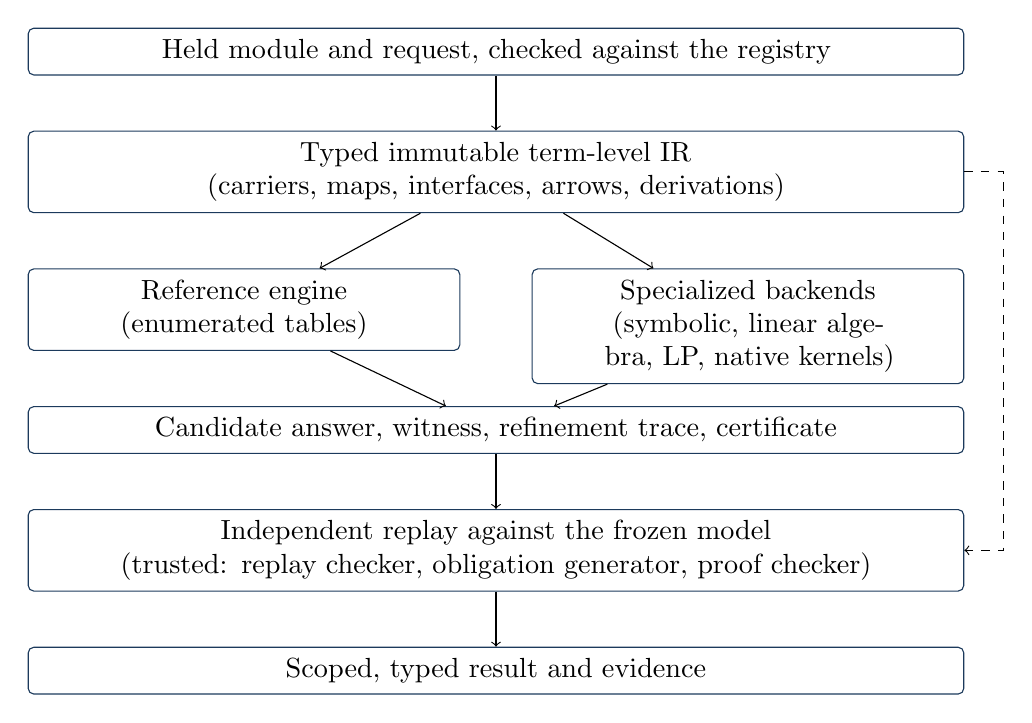
\begin{tikzpicture}[node distance=7mm, box/.style={draw=dcblue, rounded corners=2pt, align=center,
  inner sep=4pt, text width=5.2cm}, wide/.style={box, text width=11.6cm}]
\node[wide] (held) {Held module and request, checked against the registry};
\node[wide, below=of held] (ir) {Typed immutable term-level IR\\(carriers, maps, interfaces, arrows, derivations)};
\node[box, below=of ir, xshift=-3.2cm] (ref) {Reference engine\\(enumerated tables)};
\node[box, below=of ir, xshift=3.2cm] (spec) {Specialized backends\\(symbolic, linear algebra, LP, native kernels)};
\node[wide, below=of ref, xshift=3.2cm] (cand) {Candidate answer, witness, refinement trace, certificate};
\node[wide, below=of cand] (replay) {Independent replay against the frozen model\\(trusted: replay checker, obligation generator, proof checker)};
\node[wide, below=of replay] (res) {Scoped, typed result and evidence};
\draw[->] (held) -- (ir);
\draw[->] (ir) -- (ref);
\draw[->] (ir) -- (spec);
\draw[->] (ref) -- (cand);
\draw[->] (spec) -- (cand);
\draw[->] (cand) -- (replay);
\draw[->] (replay) -- (res);
\draw[->, dashed] (ir.east) -- ++(0.5,0) |- (replay.east);
\end{tikzpicture}
\caption{Proposed pipeline. Both execution paths share the admitted semantics; the dashed edge
supplies the frozen model to replay. A backend's output is not its own proof.}
\end{figure}

\emph{The IR is term-level.} Maps are terms over registered primitives; tables are one
representation of a term, chosen when the carrier is enumerated. Symbolic carriers keep their maps
as terms, which the decision-diagram, satisfiability and linear-algebra backends consume. An IR
built around dense state identifiers cannot be extended to symbolic maps later without rewriting
it, which is why the forty-bit fixture belongs to the first acceptance target.

\emph{Default algorithms are the efficient classical ones}, used within their proved scope:
functional-dependency group-bys for the current and update checks of crisp representations
(discrete code tolerance), and the same group-bys on the classes of a two-valued metric code
tolerance; Hopcroft or Paige--Tarjan
refinement for $\Pbeh$ followed by a dependency check, rather than pair-graph search, for
behavioral adequacy; splitting trees for minimal separating sequences and coarseness certificates of
deterministic machines \cite{smetsers}; $O(m\log n)$ lumping for stochastic machines
\cite{derisavi,valmari}; Krylov iteration for trace equivalence and linear realizations; and
symbolic refinement with decision diagrams as in Sigref and Storm \cite{sigref,storm}. The pair
graph remains in the definitions and in the reference engine.

\subsection{The symbolic proof boundary}

A symbolic certificate replays without the producing library, and its trusted base is stated
explicitly. The admission obligations of Section~\ref{sec:symbolic} and the constancy and stability
equations of a symbolic quotient are emitted as propositional formulas by an \emph{obligation
generator} that reads the admitted terms and the frozen semantics of the registered primitives. A
proof that a formula is unsatisfiable says nothing about whether the formula expresses the MeTTaDinC
obligation, so the generator is part of the trusted base: it is small, it is versioned with the
registry, its version is recorded in every certificate it contributes to, and it is tested by
translation validation on scaled widths, where the obligations can also be decided by enumeration.
A verified generator is an open problem (Section~\ref{sec:agenda}).

The initial pipeline is pinned. The solver CaDiCaL at release \code{rel-3.0.1}
\cite{cadical} writes a textual DRAT proof; \code{drat-trim} at commit
\code{2e3b2dc0ecf938addbd779d42877b6ed69d9a985} checks it and writes an LRAT proof with its
\code{-L} option \cite{drattrim}; and \code{cake\_lpr} at commit
\code{033aad53d1733bd4b8ca41cf6f1b5fb5d84f8de2}, a checker verified in CakeML that accepts LRAT and
its LPR extension, checks the LRAT proof against the formula and prints \code{s VERIFIED UNSAT}
\cite{cakelpr,cakelprsttt}. The formats are not interchangeable without the conversion step:
\code{cake\_lpr} does not read DRAT. Only the obligation generator and \code{cake\_lpr} are trusted;
the solver and the converter may be replaced, for instance by a solver that writes LRAT directly,
without changing the trusted base. That \code{cake\_lpr} commit is announced as its final release,
with a successor checker planned in the same repository; adopting the successor is a pin change
with its own fixture run. A verdict that reaches the result without this check, for example an
unsatisfiability answer from a solver whose proof was not replayed, is Conditional on that solver
(Section~\ref{sec:trustbase}). For maps linear over a finite field, obligations are matrix identities
replayed by multiplication, and coarseness uses a splitting tree whose tests are replayed on
concrete representatives (Proposition~\ref{prop:splitting}).

\subsection{Compilation}

Specialized execution is planned to follow Cetta's guarded supercompilation design---CettaPacks with
a multi-geometry IR and a guard lifecycle, and their approximate extension with explicit error
witnesses \cite{cettapacks}---for the kernels that dominate cost: pair and splitting-tree traversal,
signature construction, sparse block sums, Krylov iteration and finite-field elimination, once that
design is available at a pinned version. Generated language packs can orchestrate requests where
the finite-Horn projection applies, and the LLVM emitter suits pure wrapper equations. Every
specialized path is checked by the same replay as the reference path, and every performance claim
compares paths with the same semantics and arithmetic.

Three records stay separate throughout: source admission (which immutable module and request were
accepted), execution provenance (which backend, plan, arithmetic and budget produced a candidate),
and semantic evidence (why the claim holds). A content hash identifies bytes; it certifies nothing
about them.

\section{Validation and research agenda}\label{sec:agenda}

\subsection{The first release}

The first useful release is the graded deterministic core with its crisp special case, on both the
table and the symbolic backend, as fixed by the capability manifest in the registry: admission
with the symbolic obligations, the measurement and check requests for current, update, behavioral
and trace defects, the behavioral tolerance, refinement with ledgers, exact and approximate
induction with the literal-congruence obligation, the frontier on enumerated carriers,
\code{CheckAbstractionMap}, \code{Then}, \code{CheckBlockPartition}, the \code{GradedKernels} library,
two-sided and splitting-tree certificates with independent replay, the result envelope with its
binding and the assurance policy of Section~\ref{sec:trust}, and the transport rules of
Table~\ref{tab:transport}. Its acceptance fixtures are the eight-state calibration, the
receipt-packet memory, the forty-bit machines with the adversarial candidate and the reachability
scope, the deterministic hypothesis modules and the graded-closure module: $45$ manifest claims. The
same release must return Unsupported for the other $78$, including every request on the seven-state
chain and on the two stochastic modules of \code{certificate\_limits.metta}, and the conformance
suite checks those answers too. The binding rules apply in that release as well, so a request whose
premises are bound to the wrong objects is InvalidInput there even when the request itself is
Unsupported. Later stages add the stochastic and linear core, nondeterminism and
simulation, the composition kernel with hives and merges, and the Hyperseed, discovery and
integration libraries, in the order given by the guide.

\subsection{The validation package}\label{sec:validation}

The package that accompanies this specification contains the registry, twenty-one fixture files
with thirty-two modules, the claims manifest with $123$ claims, the oracle with its results and
report, the static checker, and a dependency file. The oracle recomputes every number quoted in this
document in exact arithmetic, with rationals, modulo seven or modulo two, and it uses no
floating-point computation: the calibration results and witness
bounds; packet distances, defects, ledgers, frontier, induced defect and merge errors; the closure
and bracket values; affine grades; the neural, evolutionary, transfer, regime, tick and arithmetic
numbers; the seven-state chain, including the behavioral distances $\gamma/2$ and $\gamma^2/2$, the
modal witness, trace equality, the signed realization with its intertwining equations and the
five-state positive realization; the linear composition example; both forty-bit machines on scaled
widths with the adversarial candidate and the reachability scope, and the $\F_2$ observability
dimension at width forty; the parity-triangle and beacon hives, including gauge saturation, with the
least coherent refinement proved optimal by a primal and a dual solution of its linear program,
both checked exactly; the lockout simulation; the counterexamples behind the hypotheses of the
propositions, including the unnormalized positive arrow, the indiscrete code tolerance and the
clock of a single action; the policy-class trace defect, by enumeration of all deterministic policy
trees of the horizon; and the horizon distances, tests, prefixpoints and dual post-fixpoint of the
unattained supremum. It also runs randomized checks of graded descent, the induced-machine bounds,
resumption, the trace bound of Proposition~\ref{prop:behtrace}, the induced trace bound, the linear
composition law, the per-action clock-rate screen and the restriction rule on several hundred small
machines. The checker verifies that every fixture uses
only registered declarations, requests, arguments and names, that every manifest claim names a real
fixture form and agrees with the oracle, and that the first-release expectation of each claim
follows from the registry. Neither tool runs MeTTaDinC: running the fixtures through a Cetta frontend
and comparing the results with the manifest is the implementation's acceptance step.

The dependency file pins the oracle's Python version (the oracle needs only the standard library),
the CeTTa commit and the proof pipeline, and lists the integration dependencies that are not yet
pinned: the finite OmegaPLN
interpreter, the MeTTaProN kernel IR, CettaPacks, the snapshot interfaces of MORK and PathMap beyond
the bridges present in the pinned CeTTa commit, the $\omega$PLN adapter target and the Hyperseed
proof-plan registry.

\subsection{Near-miss tests}

The most informative tests separate claims that sound alike:
\begin{itemize}
\item behavioral adequacy holds while encoded updates fail;
\item a behavioral check is refuted while every trace law agrees, and only a modal test explains it;
\item a zero current defect holds up to the observer but no literal decoder exists;
\item a horizon-one quotient fails as a stationary machine, and horizon $h$ means $h$ transitions;
\item a refutation on a carrier disappears on a forward-closed subset;
\item a zero-defect map is a homomorphism that is not a quotient;
\item the empty relation is a simulation and proves no safety property;
\item blocks that pass every local check silently omit part of the carrier;
\item equal stochastic laws disagree under a shared random seed, and equal expectations hide
different laws;
\item a trace-equivalence partition has no Markov quotient, while a five-state Markov kernel
abstraction preserves all trace laws;
\item two signed linear arrows with small residuals compose to a large one;
\item a positive candidate bounds the positive dimension from above only;
\item a value-preserving map mistranslates every executable action;
\item a coherent transfer hive has an incoherent derived kernel hive until it is saturated by its
gauge, at every member;
\item equal prior-averaged models hide a necessary signal distinction;
\item a noisy sensor report must not replace the hidden state it reports;
\item an exact transfer omits the best target action;
\item a raw separator needs an invariance argument before it refutes an equivalence;
\item a complete family search and an interrupted search support different claims;
\item a missing report and a report of neither support nor opposition differ in availability;
\item closure and compression establish neither task preservation nor lower execution cost;
\item a merge that is correct on receipt sets double counts when applied to posteriors;
\item a sampled relevance screen drops a distinction that exact refinement keeps;
\item a simulation proves a safety property that no exact quotient could;
\item an unmeasured correspondence is not a measured zero;
\item an item statistic of a machine with fewer queries is lifted to a store whose item machine has
more, and a safety result is requested along a simulation whose abstract machine is not the
request's target: both are InvalidInput, naming the mismatch;
\item a receipt stream is edited while its declared digest stays the same: InvalidInput, returned
before any count or interval, with no Estimated value;
\item both graded checks pass under an indiscrete code tolerance, and exact induction is Refuted
with a literal-congruence witness (claims C01--C03);
\item a bound on trace discrepancy holds over every fixed word and is Refuted over
observation-based policies with a policy-tree witness, while the first release answers Unsupported
(O01--O04);
\item a behavioral distance is the supremum of test values that no finite test attains, so a
measurement at precision zero is Unknown, while a horizon value, a bound below the supremum and the
discounted value are decided (U01--U04).
\end{itemize}
The lifting, safety and edited-stream entries are negative acceptance fixtures of the application
bundles: the lifting and safety fixtures belong to the live-memory guide \cite{livememory} and the
edited stream to the worked example of the open-item store \cite{wmtmexample}. They are part of the acceptance
suite in the same way
as the fixtures of this package, and the implementation guide lists the whole negative acceptance
suite with the statuses an implementation must return.

\subsection{Performance measurement}

Admission, compilation, execution, certificate production and replay are measured separately, with
the relevant scaling variables: carrier size or symbolic description size, action and query
counts, transition sparsity, rational bit length, decision-diagram size, proof-log size, matrix
dimension and observer-family size. Comparisons use the same semantic scope and arithmetic; a
floating-point approximation and an exact rational computation are different workloads unless an
approximation contract relates them.

\subsection{Open problems}

\begin{enumerate}
\item Behavioral distances for several actions. The complexity of the operator $\Phi_\gamma$ with a
maximum over actions is not settled by the single-transition results \cite{chenvbw}; exact
algorithms with bit-complexity bounds, and compact coupling certificates from policy iteration
\cite{tangvb,bacci}, remain to be worked out.
\item Frontier algorithms. The weakness--defect frontier is NP-hard in general; approximation
algorithms with guarantees for behavioral defects, and their relation to Kullback--Leibler
aggregation, are open.
\item Lower bounds for positive realizations. Certifying that no positive realization is smaller
than a given dimension is what a quantumity gap needs \cite{quantumity}; certificate formats for such
lower bounds, and their relation to nonnegative-rank bounds \cite{vavasis}, are open.
\item Graded transfer hives. Holonomies that are symmetries only up to the edge defects, least
coherent refinements and gauge saturation for graded transfer libraries need a theory and
algorithms beyond linear programming on small hives.
\item A verified obligation generator, or translation validation strong enough to remove the
generator from the trusted base.
\item Symbolic stochastic machines, with decision diagrams over rational terminals, and their
certificates.
\item Learned observers and learned predictive-state models, which enter as Estimated linear
realizations and need audit protocols.
\item Certificates under self-modification. Goal contracts, certified rewrites and dynamic closure
of the goal observer \cite{goalpreservation} are interface changes in MeTTaDinC's sense; extending the
transport rules to rewrites of the checker itself is open.
\item Partial identity tracking. Merges whose correspondences are only partly measured need an
approximation theory that degrades gracefully between the shared and fresh extremes \cite{aat}.
\end{enumerate}

\subsection{Closing}

What the language is for, in the end, is letting a system that rewrites its own descriptions---forking
its memories, merging what its copies learned, translating skills between versions of itself---ask
of each rewrite how much it forgot and whether the forgetting will matter later, and get an answer it
can check rather than an answer it must trust. There turn out to be several defensible answers to
``what can be forgotten?''---forget what no experiment will ever reveal, forget what no record of
observations will reveal, forget what a symmetry hides---and much of the design work here is in
keeping those answers from being mistaken for one another. The mathematics needed for that is
mostly old, and the distinction calculus mostly supplies a way of holding it together so the answers
compose; the executable core is small enough to build soon, and the questions it opens, about
frontiers, signed representations and self-modifying checkers, look large enough to be worth
building it for.

\begin{thebibliography}{99}\small

\bibitem{dcnotes} B. Goertzel. \emph{The Distinction Calculus: d-Forms for Hives of Reflexively Self-Modifying Systems.} Working notes, September 2026.
\bibitem{dclosure} B. Goertzel. \emph{The Distinction Calculus of Metacognitive Self-Modification: Self-models as tolerances, migrations as emergence, evaluators as hives, metacognition as a pattern of forks.} Manuscript, September 2026.
\bibitem{paperone} B. Goertzel. \emph{Task-Relevant Distinctions and Predictive Inference: Certified Observer Selection, Local Distinction Certificates, Soft Observers, and Bayesian Compression.} Manuscript, 25 September 2026.
\bibitem{quantale} B. Goertzel. \emph{Quantale Weakness: A Unifying Occam-Like Bias for AGI.} Keynote, AGI-25, August 2025.
\bibitem{cettapaper} Z. Goertzel and Oruzi. \emph{CeTTa: A Direct C Runtime for MeTTa with Verified Translation.} July 2026.
\bibitem{omegapln} The d-calculus--OmegaPLN project. \emph{OmegaPLN as a Distinction Calculus: Graded Observers, Exact Provenance, Evidence Hives, and Distinction-Guided Inference Control.} Working manuscript, 27 September 2026.
\bibitem{pab} B. Goertzel. \emph{Probably Approximately Bayesian: Fidelity of $\omega$PLN to Global Probabilistic Reasoning.} Manuscript, September 2026.
\bibitem{mettapron} \emph{MeTTaProN: a probabilistic and neural sublanguage of MeTTa.} Language specification draft, November 2026.
\bibitem{hyperseed} B. Goertzel. \emph{Hyperseed Ontology: Formal Presentation and Theoretical Development.} March 2026.
\bibitem{proofplans} \emph{A Typed Proof-Plan Language for Hyperseed Commonsense Reasoning.} Specification, September 2026.
\bibitem{aat} B. Goertzel. \emph{Approximation After Taylor: Shared Distinctions, Reflexive Remainders, and Certified Refinement in Distinction Calculus.} Manuscript, 26 September 2026.
\bibitem{plnoverlap} B. Goertzel. \emph{Overlapping Evidence in PLN as a Sharing Deformation.} Note, 26 September 2026.
\bibitem{evolearn} B. Goertzel. \emph{Evolutionary Learning in the Distinction Calculus: Behavioral Quotients, Dependency Towers, and a Schema Theorem with Certified Remainders.} Manuscript, 27 September 2026.
\bibitem{transferhives} B. Goertzel. \emph{Transfer Hives: Distinction Calculus for Compositional Planning and Certified Transfer.} Manuscript, 26 September 2026.
\bibitem{regimes} B. Goertzel. \emph{Detecting and Repairing Regime Changes: Conditional Distinctions, Sequential Evidence, and Selective Adaptation.} Manuscript, September 2026.
\bibitem{marketmaking} B. Goertzel. \emph{Market Making Across Regime Shifts: Typed changes, certified transfer, and selective repair in distinction calculus.} Manuscript, September 2026.
\bibitem{goalpreservation} B. Goertzel. \emph{Goal Preservation under Self-Modification: Distinction Contracts, Reflective Observability, and Certified Rewrites.} Manuscript, September 2026.
\bibitem{langlands} B. Goertzel. \emph{Distinction Calculus in Arithmetic Langlands: Reconstruction, Integral Comparison, and a Nonreduced Weight-One Hecke Module.} Extended manuscript, September 2026.
\bibitem{neuraldc} B. Goertzel. \emph{Neural Distinction Calculus: Finite-resolution information, behavioral geometry, and tractable SLT-style analysis.} Manuscript, September 2026.
\bibitem{codd} B. Goertzel. \emph{Cost-Aware Combinatorial Decision DAGs in Distinction Calculus.} Research draft, 12 September 2026.
\bibitem{oslf} B. Goertzel. \emph{Languages and Logics as Systems of Distinctions: A Distinction-Calculus Reconstruction of OSLF, TyLA, and TyLAA.} Manuscript, September 2026.
\bibitem{quantumity} B. Goertzel. \emph{Distinction Calculus, Observer-Relative Quantumity, and Omega Hives.} Manuscript, 27 September 2026.
\bibitem{transweave} B. Goertzel. \emph{TransWeave: Bellman--Darboux intertwining for transfer and cognitive synergy.} AGI-26 companion paper, 2026.
\bibitem{cettapacks} B. Goertzel. Design notes on CeTTa-hosted guarded supercompilation (CettaPacks, multi-geometry IR) and approximate CettaPacks. July 2026.
\bibitem{cettarepo} CeTTa contributors. CeTTa source repository, \url{https://github.com/zariuq/CeTTa}, commit \code{12da03b4b055bfecff2add505e7e1ad4125bb352}.
\bibitem{livememory} \emph{Omega Memory and Goals in MeTTaDinC, Part II: Live Memory through Summary Statistics.} Implementation guide, companion to this specification, 4 November 2026, with its validation bundle.
\bibitem{wmtmexample} \emph{Omega Memory and Goals in MeTTaDinC: WMTM's Open-Item Store, from Journal to Gate.} Worked example, companion to the live-memory guide, 4 November 2026, with its validation bundle.

\bibitem{rutten} J. J. M. M. Rutten. Universal coalgebra: a theory of systems. \emph{Theoretical Computer Science} 249(1):3--80, 2000.
\bibitem{hopcroft} J. Hopcroft. An $n\log n$ algorithm for minimizing states in a finite automaton. In \emph{Theory of Machines and Computations}, Academic Press, 1971, 189--196.
\bibitem{paigetarjan} R. Paige and R. E. Tarjan. Three partition refinement algorithms. \emph{SIAM Journal on Computing} 16(6):973--989, 1987.
\bibitem{smetsers} R. Smetsers, J. Moerman and D. N. Jansen. Minimal separating sequences for all pairs of states. In \emph{LATA 2016}, LNCS 9618, 181--193.
\bibitem{dgjp} J. Desharnais, V. Gupta, R. Jagadeesan and P. Panangaden. Metrics for labelled Markov processes. \emph{Theoretical Computer Science} 318(3):323--354, 2004.
\bibitem{vbw} F. van Breugel and J. Worrell. An algorithm for quantitative verification of probabilistic transition systems. In \emph{CONCUR 2001}, LNCS 2154, 336--350.
\bibitem{ferns} N. Ferns, P. Panangaden and D. Precup. Metrics for finite Markov decision processes. In \emph{UAI 2004}, 162--169.
\bibitem{chenvbw} D. Chen, F. van Breugel and J. Worrell. On the complexity of computing probabilistic bisimilarity. In \emph{FoSSaCS 2012}, LNCS 7213, 437--451.
\bibitem{chenkiefer} T. Chen and S. Kiefer. On the total variation distance of labelled Markov chains. In \emph{CSL-LICS 2014}, 33:1--33:10.
\bibitem{bacci} G. Bacci, G. Bacci, K. G. Larsen and R. Mardare. On-the-fly exact computation of bisimilarity distances. In \emph{TACAS 2013}, LNCS 7795, 1--15.
\bibitem{tangvb} Q. Tang and F. van Breugel. Computing probabilistic bisimilarity distances via policy iteration. In \emph{CONCUR 2016}, LIPIcs 59, 22:1--22:15.
\bibitem{kemenysnell} J. G. Kemeny and J. L. Snell. \emph{Finite Markov Chains}. Van Nostrand, 1960.
\bibitem{larsenskou} K. G. Larsen and A. Skou. Bisimulation through probabilistic testing. \emph{Information and Computation} 94(1):1--28, 1991.
\bibitem{buchholz} P. Buchholz. Exact and ordinary lumpability in finite Markov chains. \emph{Journal of Applied Probability} 31(1):59--75, 1994.
\bibitem{franceschinis} G. Franceschinis and R. R. Muntz. Bounds for quasi-lumpable Markov chains. \emph{Performance Evaluation} 20:223--243, 1994.
\bibitem{derisavi} S. Derisavi, H. Hermanns and W. H. Sanders. Optimal state-space lumping in Markov chains. \emph{Information Processing Letters} 87(6):309--315, 2003.
\bibitem{valmari} A. Valmari and G. Franceschinis. Simple $O(m\log n)$ time Markov chain lumping. In \emph{TACAS 2010}, LNCS 6015, 38--52.
\bibitem{dmm} K. Deng, P. G. Mehta and S. P. Meyn. Optimal Kullback--Leibler aggregation via spectral theory of Markov chains. \emph{IEEE Transactions on Automatic Control} 56(12):2793--2808, 2011.
\bibitem{geiger} B. C. Geiger, T. Petrov, G. Kubin and H. Koeppl. Optimal Kullback--Leibler aggregation via information bottleneck. \emph{IEEE Transactions on Automatic Control} 60(4):1010--1022, 2015.
\bibitem{maxecp} J. Dessmark, J. Jansson, A. Lingas, E.-M. Lundell and M. Persson. On the approximability of maximum and minimum edge clique partition problems. \emph{International Journal of Foundations of Computer Science} 18(2):217--226, 2007.
\bibitem{schutzenberger} M.-P. Sch\"utzenberger. On the definition of a family of automata. \emph{Information and Control} 4(2--3):245--270, 1961.
\bibitem{tzeng} W.-G. Tzeng. A polynomial-time algorithm for the equivalence of probabilistic automata. \emph{SIAM Journal on Computing} 21(2):216--227, 1992.
\bibitem{kiefer} S. Kiefer, A. S. Murawski, J. Ouaknine, B. Wachter and J. Worrell. Language equivalence for probabilistic automata. In \emph{CAV 2011}, LNCS 6806, 526--540.
\bibitem{jaeger} H. Jaeger. Observable operator models for discrete stochastic time series. \emph{Neural Computation} 12(6):1371--1398, 2000.
\bibitem{psr} M. L. Littman, R. S. Sutton and S. Singh. Predictive representations of state. In \emph{Advances in Neural Information Processing Systems 14}, 2002.
\bibitem{vavasis} S. A. Vavasis. On the complexity of nonnegative matrix factorization. \emph{SIAM Journal on Optimization} 20(3):1364--1377, 2009.
\bibitem{milner} R. Milner. \emph{Communication and Concurrency}. Prentice Hall, 1989.
\bibitem{hhk} M. R. Henzinger, T. A. Henzinger and P. W. Kopke. Computing simulations on finite and infinite graphs. In \emph{FOCS 1995}, 453--462.
\bibitem{hennessymilner} M. Hennessy and R. Milner. Algebraic laws for nondeterminism and concurrency. \emph{Journal of the ACM} 32(1):137--161, 1985.
\bibitem{cleaveland} R. Cleaveland. On automatically explaining bisimulation inequivalence. In \emph{CAV 1990}, LNCS 531, 364--372.
\bibitem{martensgroote} J. Martens and J. F. Groote. Computing minimal distinguishing Hennessy--Milner formulas is NP-hard, but variants are tractable. In \emph{CONCUR 2023}, LIPIcs 279, 32:1--32:17.
\bibitem{kanellakis} P. C. Kanellakis and S. A. Smolka. CCS expressions, finite state processes, and three problems of equivalence. \emph{Information and Computation} 86(1):43--68, 1990.
\bibitem{antichains} M. De Wulf, L. Doyen, T. A. Henzinger and J.-F. Raskin. Antichains: a new algorithm for checking universality of finite automata. In \emph{CAV 2006}, LNCS 4144, 17--30.
\bibitem{bonchipous} F. Bonchi and D. Pous. Checking NFA equivalence with bisimulations up to congruence. In \emph{POPL 2013}, 457--468.
\bibitem{cousot} P. Cousot and R. Cousot. Abstract interpretation: a unified lattice model for static analysis of programs by construction or approximation of fixpoints. In \emph{POPL 1977}, 238--252.
\bibitem{cegar} E. Clarke, O. Grumberg, S. Jha, Y. Lu and H. Veith. Counterexample-guided abstraction refinement. In \emph{CAV 2000}, LNCS 1855, 154--169.
\bibitem{copar} H.-P. Deifel, S. Milius, L. Schr\"oder and T. Wi\ss{}mann. Generic partition refinement and weighted tree automata. In \emph{FM 2019}, LNCS 11800, 280--297.
\bibitem{copar2} T. Wi\ss{}mann, U. Dorsch, S. Milius and L. Schr\"oder. Efficient and modular coalgebraic partition refinement. \emph{Logical Methods in Computer Science} 16(1):8, 2020.
\bibitem{explaining} T. Wi\ss{}mann, S. Milius and L. Schr\"oder. Explaining behavioural inequivalence generically in quasilinear time. In \emph{CONCUR 2021}, LIPIcs 203, 32:1--32:18.
\bibitem{niuspivak} N. Niu and D. I. Spivak. \emph{Polynomial Functors: A Mathematical Theory of Interaction}. arXiv:2312.00990, 2023.
\bibitem{lawvere} F. W. Lawvere. Metric spaces, generalized logic, and closed categories. \emph{Rendiconti del Seminario Matematico e Fisico di Milano} 43:135--166, 1973.
\bibitem{sigref} R. Wimmer, M. Herbstritt, H. Hermanns, K. Strampp and B. Becker. Sigref: a symbolic bisimulation tool box. In \emph{ATVA 2006}, LNCS 4218, 477--492.
\bibitem{storm} C. Hensel, S. Junges, J.-P. Katoen, T. Quatmann and M. Volk. The probabilistic model checker Storm. \emph{International Journal on Software Tools for Technology Transfer} 24:589--610, 2022.
\bibitem{cadical} A. Biere and contributors. CaDiCaL SAT solver, \url{https://github.com/arminbiere/cadical}, release \code{rel-3.0.1}, commit \code{c60730422e758ef1cebe7aeddf2dda31c996bf04}.
\bibitem{drattrim} N. Wetzler, M. J. H. Heule and W. A. Hunt. DRAT-trim: efficient checking and trimming using expressive clausal proofs. In \emph{SAT 2014}, LNCS 8561, 422--429. Source: \url{https://github.com/marijnheule/drat-trim}.
\bibitem{cakelpr} Y. K. Tan, M. J. H. Heule and M. O. Myreen. cake\_lpr: verified propagation redundancy checking in CakeML. In \emph{TACAS 2021}, LNCS 12652, 223--241.
\bibitem{cakelprsttt} Y. K. Tan, M. J. H. Heule and M. O. Myreen. Verified propagation redundancy and compositional UNSAT checking in CakeML. \emph{International Journal on Software Tools for Technology Transfer} 25(2):167--184, 2023. Binaries: \url{https://github.com/tanyongkiam/cake_lpr}.
\bibitem{cik} A. Chistov, G. Ivanyos and M. Karpinski. Polynomial time algorithms for modules over finite dimensional algebras. In \emph{ISSAC 1997}, 68--74.
\bibitem{brooksbankluks} P. A. Brooksbank and E. M. Luks. Testing isomorphism of modules. \emph{Journal of Algebra} 320(11):4020--4029, 2008.
\bibitem{belnap} N. D. Belnap. A useful four-valued logic. In \emph{Modern Uses of Multiple-Valued Logic}, Reidel, 1977, 5--37.
\bibitem{ginsberg} M. L. Ginsberg. Multivalued logics: a uniform approach to reasoning in artificial intelligence. \emph{Computational Intelligence} 4(3):265--316, 1988.
\bibitem{arieliavron} O. Arieli and A. Avron. Reasoning with logical bilattices. \emph{Journal of Logic, Language and Information} 5(1):25--63, 1996.
\bibitem{hoeffding48} W. Hoeffding. A class of statistics with asymptotically normal distribution. \emph{Annals of Mathematical Statistics} 19(3):293--325, 1948.
\bibitem{hoeffding63} W. Hoeffding. Probability inequalities for sums of bounded random variables. \emph{Journal of the American Statistical Association} 58(301):13--30, 1963.
\bibitem{howard} S. R. Howard, A. Ramdas, J. McAuliffe and J. Sekhon. Time-uniform, nonparametric, nonasymptotic confidence sequences. \emph{Annals of Statistics} 49(2):1055--1080, 2021.
\bibitem{ramdas} A. Ramdas, P. Gr\"unwald, V. Vovk and G. Shafer. Game-theoretic statistics and safe anytime-valid inference. \emph{Statistical Science} 38(4):576--601, 2023.

\end{thebibliography}

\appendix

\section{Declaration registry}\label{app:grammar}
This appendix and the next are generated from \code{registry/mettadinc\_registry.json}. Required fields are listed plainly, optional fields in brackets, and repeatable fields with a trailing $+$. Every declaration takes its name as the first positional argument.
{\footnotesize\begin{longtable}{>{\raggedright\arraybackslash}p{3.0cm}>{\raggedright\arraybackslash}p{2.0cm}>{\raggedright\arraybackslash}p{9.0cm}}
\toprule Declaration & Library & Fields and body\\ \midrule \endhead
\code{Type} & Core & \emph{type}\\
\code{Record} & Core & \emph{fields}\\
\code{Const} & Core & \emph{type}, \emph{value}\\
\code{Carrier} & Core & \code{Of}, \emph{carrier-expr}\\
\code{Map} & Core & \code{From}, \code{To}, \emph{map-body}\\
\code{Tolerance} & Core & \code{On}, \emph{tolerance-body}\\
\code{Measure} & Core & \code{On}, \emph{measure-body}\\
\code{PairLaw} & Core & \code{Independent}, \code{Diagonal}\\
\code{TransitionKernel} & Core & \code{From}, \code{To}, [\code{Row}$+$], [\code{Import}]\\
\code{Machine} & Core & \code{States}, [\code{Observe}$+$], [\code{Action}$+$], [\code{Merge}$+$], [\code{Available}$+$], [\code{Bag}]\\
\code{Representation} & Core & \code{Of}, \code{Encode}, [\code{Codes}]\\
\code{AbstractionMap} & Core & \code{Source}, \code{Target}, \code{Map}\\
\code{Snapshot} & Core & \code{Space}, \code{Digest}, [\code{Revision}]\\
\code{Derive} & Core & \emph{request}\\
\code{BlockPartition} & Core & \code{On}, \code{Block}$+$, [\code{Successor}$+$]\\
\code{LinearRealization} & Linear & \code{Dimension}, \code{Operator}$+$, \code{Projector}$+$, \code{Final}\\
\code{LinearArrow} & Linear & \code{Source}, \code{Target}, \code{Matrix}, \code{Kind}\\
\code{Simulation} & Simulation & \code{Source}, \code{Target}, \code{Relation}, [\code{Order}]\\
\code{Relation} & Simulation & \code{From}, \code{To}, \code{Pairs}\\
\code{Scheduler} & Simulation & \code{Rule}\\
\code{MethodSystem} & Transfers & \code{States}, \code{Methods}, \code{Response}, [\code{Observe}$+$]\\
\code{Transfer} & Transfers & \code{Source}, \code{Target}, \code{StatePullback}, \code{MethodPushforward}, [\code{Responses}]\\
\code{Symmetry} & Transfers & \code{Of}, \code{States}, \code{Methods}\\
\code{CrossKernel} & Hives & \code{Left}, \code{Right}, \code{Entries}\\
\code{KernelHive} & Hives & \code{Member}$+$, \code{Correspondence}$+$, [\code{Weights}]\\
\code{TransferHive} & Hives & \code{Member}$+$, \code{Edge}$+$, \code{Cycle}$+$, [\code{Gauge}$+$], [\code{Weights}]\\
\code{Implementation} & Contracts & \code{Ideal}, \code{Actual}, \code{Audit}, \code{InputDistance}, \code{OutputDistance}\\
\code{ObserverFamily} & Discovery & \code{On}, \code{Returns}, \code{Generate}\\
\code{ObserverSource} & Discovery & \code{Procedure}, \code{On}\\
\code{ReportSystem} & Neural & \code{Input}, \code{ReportType}, \code{Encoder}, \code{Readout}\\
\code{DecisionModel} & Decisions & \code{States}, \code{Actions}, \code{RewardLaw}, [\code{Prior}]\\
\code{ObservationMethod} & Decisions & \code{Channel}, \code{Cost}\\
\code{Archive} & Search & \code{Machine}, \code{Key}, \code{Start}, \code{ParentChoice}\\
\code{Schema} & Hyperseed & \code{Parameters}, \code{Build}\\
\code{Method} & Hyperseed & \code{Parameters}, \code{Returns}, \code{Body}\\
\code{DescriptionSystem} & Hyperseed & \code{Description}$+$, \code{Decoder}, \code{Cost}, \code{Baseline}\\
\code{PatternWitness} & Hyperseed & \code{System}, \code{Target}, \code{Description}\\
\bottomrule\end{longtable}}
\section{Requests, results and statuses}\label{app:schemas}
Every request can also return the base statuses Conditional, Unknown, Unsupported, InvalidInput. Keyed arguments are shown with their defaults; an argument without a default is optional unless marked required (req). The last column marks the requests in the first-release capability manifest, which covers deterministic dynamics only.
{\scriptsize\begin{longtable}{>{\raggedright\arraybackslash}p{4.4cm}>{\raggedright\arraybackslash}p{6.8cm}>{\raggedright\arraybackslash}p{1.9cm}>{\raggedright\arraybackslash}p{0.5cm}}
\toprule Request (library) and result type & Arguments & Statuses & R1\\ \midrule \endhead
\code{MeasureNow} (Core)\newline$\to$ \code{DefectMeasurement} & \emph{subject}, \code{Precision}=\code{0}, [\code{Budget}] & Che & yes\\
\code{CheckNow} (Core)\newline$\to$ \code{DefectCheck} & \emph{subject}, \code{Within}=\code{0}, [\code{Budget}] & Che, Ref & yes\\
\code{MeasureUpdates} (Core)\newline$\to$ \code{DefectMeasurement} & \emph{subject}, \code{Precision}=\code{0}, [\code{Budget}] & Che & yes\\
\code{CheckUpdates} (Core)\newline$\to$ \code{DefectCheck} & \emph{subject}, \code{Within}=\code{0}, [\code{Budget}] & Che, Ref & yes\\
\code{MeasureBehavioral} (Core)\newline$\to$ \code{DefectMeasurement} & \emph{subject}, \code{Discount}=\code{1}, \code{Horizon}=\code{AllFiniteWords}, \code{Precision}=\code{0}, [\code{Budget}] & Che & yes\\
\code{CheckBehavioral} (Core)\newline$\to$ \code{DefectCheck} & \emph{subject}, \code{Discount}=\code{1}, \code{Horizon}=\code{AllFiniteWords}, \code{Within}=\code{0}, [\code{Budget}] & Che, Ref & yes\\
\code{MeasureTrace} (Core)\newline$\to$ \code{DefectMeasurement} & \emph{subject}, \code{Horizon}=\code{AllFiniteWords}, \code{Policies}=\code{Words}, \code{Precision}=\code{0}, [\code{Budget}] & Che & yes\\
\code{CheckTrace} (Core)\newline$\to$ \code{DefectCheck} & \emph{subject}, \code{Horizon}=\code{AllFiniteWords}, \code{Policies}=\code{Words}, \code{Within}=\code{0}, [\code{Budget}] & Che, Ref & yes\\
\code{Defects} (Core)\newline$\to$ \code{DefectRecord} & \emph{subject}, \code{Discount}=\code{1}, \code{Horizon}=\code{AllFiniteWords}, \code{Precision}=\code{0}, [\code{Budget}] & Che & yes\\
\code{BehavioralTolerance} (Core)\newline$\to$ \code{ToleranceResult} & \emph{machine}, \code{Discount}=\code{1}, \code{Horizon}=\code{AllFiniteWords}, \code{Precision}=\code{0}, [\code{Budget}] & Che & yes\\
\code{Refine} (Core)\newline$\to$ \code{Refinement} & \emph{subject}, \code{Preserve}=\code{Encoding}, \code{Until}=\code{Stable}, [\code{Under}], [\code{Budget}] & Che & yes\\
\code{MinimizeForQueries} (Core)\newline$\to$ \code{Refinement} & \emph{machine}, [\code{Under}], [\code{Budget}] & Che & yes\\
\code{InduceExact} (Core)\newline$\to$ \code{ExactAbstraction} & \emph{subject}, [\code{Budget}] & Che, Ref & yes\\
\code{InduceApprox} (Core)\newline$\to$ \code{ApproxAbstraction} & \emph{subject}, \code{Representatives}=\code{Center}, \code{Discount}=\code{1}, \code{Horizon}=\code{AllFiniteWords}, [\code{Within}], [\code{Budget}] & Che, Ref & yes\\
\code{WeakestWithin} (Core)\newline$\to$ \code{Frontier} & \emph{machine}, \code{Within} (req), \code{Kind}=\code{Behavioral}, \code{Discount}=\code{1}, \code{Under} (req), \code{Search}=\code{Exhaustive}, [\code{Budget}] & Che & yes\\
\code{CheckAbstractionMap} (Core)\newline$\to$ \code{CheckedAbstractionMap} & \emph{arrow}, [\code{Budget}] & Che, Ref & yes\\
\code{Then} (Core)\newline$\to$ \code{ComposedArrow} & \emph{first}, \emph{second} & Che & yes\\
\code{CheckBlockPartition} (Core)\newline$\to$ \code{BlockPartitionCheck} & \emph{partition}, \code{Of} (req), [\code{Budget}] & Che, Ref & yes\\
\code{SamePartition} (Core)\newline$\to$ \code{Verdict} & \emph{left}, \emph{right} & Che, Ref & yes\\
\code{MinimalLinear} (Linear)\newline$\to$ \code{LinearMinimum} & \emph{machine}, [\code{Budget}] & Che & --\\
\code{TracePartition} (Linear)\newline$\to$ \code{PartitionResult} & \emph{machine}, [\code{Budget}] & Che & --\\
\code{CheckLinearArrow} (Linear)\newline$\to$ \code{CheckedLinearArrow} & \emph{arrow}, \code{Norm}=\code{InfinityOperator}, [\code{Budget}] & Che, Ref & --\\
\code{PositiveRealization} (Linear)\newline$\to$ \code{PositiveDimension} & \emph{machine}, \code{Candidate} (req), [\code{Budget}] & Che, Ref & --\\
\code{CheckSimulation} (Simulation)\newline$\to$ \code{CheckedSimulation} & \emph{simulation}, [\code{Budget}] & Che, Ref & --\\
\code{CheckSafety} (Simulation)\newline$\to$ \code{SafetyResult} & \emph{target}, \code{Never} (req), \code{Via} (req), \code{Init} (req), [\code{Budget}] & Che, Ref & --\\
\code{Outcomes} (Simulation)\newline$\to$ \code{OutcomeSet} & \emph{machine}, \code{From} (req), \code{After} (req), \code{Observe} (req) & Che & --\\
\code{OutcomeProbability} (Simulation)\newline$\to$ \code{Scalar} & \emph{machine}, \code{From} (req), \code{After} (req), \code{Event} (req), \code{Scheduler} (req) & Che & --\\
\code{PathClosure} (GradedKernels)\newline$\to$ \code{KernelResult} & \emph{kernel}, \code{Algebra}=\code{Lukasiewicz01} & Che & yes\\
\code{Threshold} (GradedKernels)\newline$\to$ \code{RelationResult} & \emph{kernel}, \code{AtLeast} (req) & Che & yes\\
\code{Bracket} (GradedKernels)\newline$\to$ \code{Scalar} & \emph{kernel}, \code{Under} (req) & Che & yes\\
\code{Delta} (GradedKernels)\newline$\to$ \code{Scalar} & \code{From} (req), \code{To} (req) & Che & yes\\
\code{CheckTransitive} (GradedKernels)\newline$\to$ \code{Verdict} & \emph{kernel}, \code{Algebra}=\code{Lukasiewicz01} & Che, Ref & yes\\
\code{CheckImplementation} (Contracts)\newline$\to$ \code{CheckedImplementationContract} & \emph{implementation}, \code{Grade} (req) & Che, Ref & --\\
\code{ThenContracts} (Contracts)\newline$\to$ \code{CheckedImplementationContract} & \emph{first}, \emph{second} & Che & --\\
\code{CheckTransfer} (Transfers)\newline$\to$ \code{CheckedTransfer} & \emph{transfer}, \code{Within}=\code{0}, \code{Metric}=\code{RewardLawTV} & Che, Ref & --\\
\code{ComposeTransfers} (Transfers)\newline$\to$ \code{CheckedTransfer} & \emph{transfers} & Che & --\\
\code{CheckValuePullback} (Transfers)\newline$\to$ \code{ValueCertificate} & \emph{transfer} & Che, Ref & --\\
\code{LibraryGap} (Transfers)\newline$\to$ \code{Scalar} & \emph{transfer} & Che & --\\
\code{CheckKernelCoherence} (Hives)\newline$\to$ \code{HiveCoherence} & \emph{hive} & Che, Ref & --\\
\code{Holonomy} (Hives)\newline$\to$ \code{HiveKernel} & \emph{hive}, \code{Cycle} (req) & Che & --\\
\code{ConsensusCost} (Hives)\newline$\to$ \code{Scalar} & \emph{hive} & Che & --\\
\code{CompleteHive} (Hives)\newline$\to$ \code{HiveResult} & \emph{hive} & Che & --\\
\code{LeastCoherentRefinement} (Hives)\newline$\to$ \code{HiveResult} & \emph{hive}, \code{Search}=\code{LinearProgram}, [\code{Budget}] & Che & --\\
\code{CheckTransferHive} (Hives)\newline$\to$ \code{TransferHiveCoherence} & \emph{hive} & Che, Ref & --\\
\code{KernelOf} (Hives)\newline$\to$ \code{DerivedKernelHive} & \emph{hive}, \code{Saturate}=\code{None} & Che & --\\
\code{SeekSeparator} (Discovery)\newline$\to$ \code{SeparatorResult} & \code{Pair} (req), \code{Family} (req), \code{Require} (req), \code{Order}=\code{GeneratedOrder}, [\code{Budget}] & Che & --\\
\code{CheckObserverInvariance} (Discovery)\newline$\to$ \code{InvarianceResult} & \emph{family}, \code{Under} (req), \code{Method} (req) & Che, Ref & --\\
\code{DecideEquivalence} (Discovery)\newline$\to$ \code{EquivalenceDecision} & \emph{source}, \code{Pair} (req), [\code{Budget}] & Che, Ref & --\\
\code{ClockRates} (Discovery)\newline$\to$ \code{ClockRateTable} & \emph{machine}, \code{Under} (req), \code{Library} (req), \code{Kind}=\code{Mean}, [\code{Budget}] & Che, Est & --\\
\code{ConeOfInfluence} (Discovery)\newline$\to$ \code{CoordinateSet} & \emph{machine} & Che & --\\
\code{CompareDistinctions} (Neural)\newline$\to$ \code{DistinctionComparison} & \emph{old}, \emph{new}, \code{Under} (req) & Che, Est & --\\
\code{AuditIntervention} (Neural)\newline$\to$ \code{MetricTable} & \code{Systems} (req), \code{Intervention} (req), \code{Task} (req), \code{Under} (req), \code{Metric} (req) & Che, Est & --\\
\code{AverageModel} (Decisions)\newline$\to$ \code{AveragedModel} & \emph{model}, \code{Under} (req) & Che & --\\
\code{CheckEqual} (Decisions)\newline$\to$ \code{Verdict} & \emph{left}, \emph{right} & Che, Ref & --\\
\code{OptimizePolicy} (Decisions)\newline$\to$ \code{PolicyValue} & \emph{model}, [\code{Through}], \code{Under} (req) & Che & --\\
\code{EvaluatePolicy} (Decisions)\newline$\to$ \code{PolicyValue} & \emph{model}, \code{With} (req), \code{Under} (req) & Che & --\\
\code{ExpectedProposals} (Search)\newline$\to$ \code{Scalar} & \emph{archive}, \code{Until} (req) & Che & --\\
\code{FindCheapestDescription} (Hyperseed)\newline$\to$ \code{DescriptionResult} & \emph{system}, \code{Target} (req) & Che & --\\
\code{CheckPatternWitness} (Hyperseed)\newline$\to$ \code{Verdict} & \emph{witness} & Che, Ref & --\\
\bottomrule\end{longtable}}
Status abbreviations: Che Checked, Ref Refuted, Est Estimated. Result types and their fields:
{\footnotesize\begin{longtable}{>{\raggedright\arraybackslash}p{4.9cm}>{\raggedright\arraybackslash}p{9.1cm}}
\toprule Result type & Fields (a trailing ? marks a field present only in some outcomes)\\ \midrule \endhead
\code{DefectMeasurement} & \code{Defect}: Interval, \code{Equality}: enum:Literal|\allowbreak{}Observer, \code{Decoders}: Map?, \code{Updates}: Map?, \code{Witness}: Witness?, \code{Certificate}: Certificate\\
\code{DefectCheck} & \code{Defect}: Interval, \code{Bound}: Rational, \code{Equality}: enum:Literal|\allowbreak{}Observer, \code{Decoders}: Map?, \code{Updates}: Map?, \code{Witness}: Witness?, \code{Certificate}: Certificate\\
\code{DefectRecord} & \code{Now}: DefectMeasurement, \code{Updates}: DefectMeasurement, \code{Behavioral}: DefectMeasurement, \code{Trace}: DefectMeasurement?\\
\code{BlockPartitionCheck} & \code{Obligation}: enum:Coverage|\allowbreak{}Disjointness|\allowbreak{}Membership|\allowbreak{}Constancy|\allowbreak{}Stability|\allowbreak{}Closure|\allowbreak{}Reachability?, \code{Witness}: Witness?, \code{Certificate}: Certificate\\
\code{PartitionResult} & \code{Partition}: Partition, \code{Certificate}: Certificate\\
\code{ToleranceResult} & \code{Tolerance}: Tolerance, \code{Certificate}: Certificate\\
\code{Refinement} & \code{Representation}: Representation, \code{Partition}: Partition, \code{Ledger}: Ledger, \code{Certificate}: Certificate\\
\code{ExactAbstraction} & \code{Machine}: Machine?, \code{AbstractionMap}: CheckedAbstractionMap?, \code{Decoders}: Map?, \code{Updates}: Map?, \code{Equality}: enum:Literal|\allowbreak{}Observer?, \code{Obligation}: enum:Current|\allowbreak{}Update|\allowbreak{}Congruence?, \code{Witness}: Witness?, \code{Certificate}: Certificate\\
\code{ApproxAbstraction} & \code{Machine}: Machine, \code{Selector}: Map, \code{Radius}: Rational, \code{Defect}: Interval, \code{Bound}: Rational?, \code{AbstractionMap}: CheckedGradedArrow, \code{Witness}: Witness?, \code{Certificate}: Certificate\\
\code{Frontier} & \code{Representation}: Representation, \code{Partition}: Partition, \code{Weakness}: Rational, \code{Defect}: Interval, \code{Optimality}: enum:Checked|\allowbreak{}Unknown, \code{Certificate}: Certificate\\
\code{CheckedAbstractionMap} & \code{Kind}: enum:Quotient|\allowbreak{}Homomorphism, \code{Map}: Map, \code{Source}: Machine, \code{Target}: Machine, \code{Certificate}: Certificate\\
\code{CheckedGradedArrow} & \code{Map}: Map, \code{Defect}: Interval, \code{Discount}: Rational, \code{Certificate}: Certificate\\
\code{ComposedArrow} & \code{Arrow}: Arrow, \code{Grade}: Grade, \code{Certificate}: Certificate\\
\code{Verdict} & \code{Witness}: Witness?, \code{Certificate}: Certificate\\
\code{LinearMinimum} & \code{Dimension}: Nat, \code{Basis}: TestBasis, \code{Realization}: LinearRealization, \code{SeparatingTests}: TestList, \code{Certificate}: Certificate\\
\code{CheckedLinearArrow} & \code{Kind}: enum:Positive|\allowbreak{}Signed, \code{Lambda}: Rational, \code{Rho}: Rational, \code{Certificate}: Certificate\\
\code{PositiveDimension} & \code{Lower}: Nat, \code{Upper}: Nat, \code{LowerEvidence}: enum:SignedMinimum|\allowbreak{}PositiveLowerCertificate, \code{Realization}: LinearArrow, \code{Certificate}: Certificate\\
\code{CheckedSimulation} & \code{Relation}: Relation, \code{Certificate}: Certificate\\
\code{SafetyResult} & \code{InitialCoverage}: Certificate, \code{AbstractScope}: StateSet, \code{Witness}: Witness?, \code{Certificate}: Certificate\\
\code{OutcomeSet} & \code{Outcomes}: ValueSet\\
\code{Scalar} & \code{Value}: Rational\\
\code{KernelResult} & \code{Kernel}: Tolerance, \code{Certificate}: Certificate\\
\code{RelationResult} & \code{Relation}: Relation\\
\code{CheckedImplementationContract} & \code{Grade}: Grade, \code{Certificate}: Certificate, \code{Witness}: Witness?\\
\code{CheckedTransfer} & \code{Transfer}: Transfer, \code{Defect}: Interval, \code{Metric}: enum:RewardLawTV|\allowbreak{}ExpectedReward, \code{Certificate}: Certificate, \code{Witness}: Witness?\\
\code{ValueCertificate} & \code{Values}: Table, \code{Certificate}: Certificate\\
\code{HiveCoherence} & \code{Holonomy}: Kernel?, \code{Witness}: Witness?, \code{Certificate}: Certificate\\
\code{HiveKernel} & \code{Kernel}: Tolerance\\
\code{HiveResult} & \code{Hive}: KernelHive, \code{Cost}: Rational, \code{Optimality}: enum:Checked|\allowbreak{}Unknown, \code{Certificate}: Certificate\\
\code{TransferHiveCoherence} & \code{Holonomies}: TransferList, \code{GaugeEvidence}: Certificate, \code{Witness}: Witness?\\
\code{DerivedKernelHive} & \code{Hive}: KernelHive, \code{Saturation}: enum:Gauge|\allowbreak{}None, \code{Certificate}: Certificate\\
\code{SeparatorResult} & \code{Observer}: Expr, \code{Evaluations}: Table, \code{Invariance}: Certificate\\
\code{InvarianceResult} & \code{Derivation}: Certificate\\
\code{EquivalenceDecision} & \code{Conjugator}: Matrix?, \code{HomDimensions}: Table?, \code{Certificate}: Certificate\\
\code{ClockRateTable} & \code{Rates}: Table, \code{Exact}: CoordinateSet, \code{Hypotheses}: Certificate\\
\code{CoordinateSet} & \code{Coordinates}: CoordinateSet\\
\code{DistinctionComparison} & \code{MassOld}: Rational, \code{MassNew}: Rational, \code{Creation}: Rational, \code{Erasure}: Rational, \code{Turnover}: Rational\\
\code{MetricTable} & \code{Table}: Table\\
\code{PolicyValue} & \code{Value}: Rational, \code{Policy}: Table?\\
\code{AveragedModel} & \code{Model}: DecisionModel\\
\code{DescriptionResult} & \code{Description}: Name, \code{Cost}: Rational, \code{Optimality}: enum:Checked|\allowbreak{}Unknown\\
\bottomrule\end{longtable}}
Every result, whatever its request, has the envelope below; its \code{Value} field holds the fields of the result type listed above (Section~\ref{sec:trust}).
{\footnotesize\begin{longtable}{>{\raggedright\arraybackslash}p{3.0cm}>{\raggedright\arraybackslash}p{11.4cm}}
\toprule Envelope field & Content\\ \midrule \endhead
\code{Status} & one of the seven statuses\\ \addlinespace[3pt]
\code{Claim} & the claim kind,\allowbreak{} its bound or precision,\allowbreak{} and the observation equality (Literal or Observer)\\ \addlinespace[3pt]
\code{Binding} & the exact objects the claim is about: the module digest and the names of the subject declarations; for arrows,\allowbreak{} simulations and transfers the source and target model identities; the interface checked against (queries with their value tolerances,\allowbreak{} actions with their update kinds,\allowbreak{} merges)\\ \addlinespace[3pt]
\code{Scope} & initial states,\allowbreak{} reachable-state scope,\allowbreak{} horizon,\allowbreak{} discount,\allowbreak{} and policy class (Words or ObservationBased)\\ \addlinespace[3pt]
\code{Value} & the fields of the request's registered result type\\ \addlinespace[3pt]
\code{Estimate} & present on Estimated results and on results derived from them: (Estimate (Estimand e) (Population p) (Selection rule) (Policy digest) (Estimator m) (Protocol pr) (SampleSize n) (Error epsilon delta) (Dependence assumptions) (Combination rule)); the estimand is stated as a function of the population,\allowbreak{} and the policy is the version under which the rows were produced\\ \addlinespace[3pt]
\code{Evidence} & the certificate kind and digest,\allowbreak{} the digests of the streams and snapshots read,\allowbreak{} and agreed\_by\\ \addlinespace[3pt]
\code{agreed\_by} & inside Evidence: other backends that reached the same verdict on an independently written encoding,\allowbreak{} as (solver version logic encoding-digest); evidence only,\allowbreak{} it discharges no assumption\\ \addlinespace[3pt]
\code{Assumptions} & the undischarged assumptions,\allowbreak{} for example (TrustedBackend cvc5 1.4.2 QF\_LRA sha256:...); a derived result lists the union of its premises' assumptions\\ \addlinespace[3pt]
\code{Assurance} & the grounds of the status: Exact or Replayed for Checked,\allowbreak{} Witness for Refuted,\allowbreak{} Statistical for Estimated; for Conditional,\allowbreak{} the grounds of its undischarged assumptions (TrustedBackend,\allowbreak{} Assumed,\allowbreak{} Statistical)\\ \addlinespace[3pt]
\code{Dependencies} & the premise results,\allowbreak{} by digest\\ \addlinespace[3pt]
\code{Method} & the backend,\allowbreak{} algorithm and arithmetic that produced the candidate (execution provenance)\\ \addlinespace[3pt]
\code{Resources} & the work done,\allowbreak{} and the certified interval of an Unknown result\\ \addlinespace[3pt]
\bottomrule\end{longtable}}
The assurance policy assigns each status on one ground, and consumers declare which results they accept: a result is Checked only on the grounds Exact or Replayed,\allowbreak{} Refuted only on the ground Witness,\allowbreak{} Estimated only on the ground Statistical,\allowbreak{} and Conditional when it rests on an unreplayed backend answer,\allowbreak{} a declared assumption,\allowbreak{} an Estimated premise or a Conditional premise,\allowbreak{} in every request and library; a value of a behavioral or trace distance is Checked only through the registered certificate kinds (certificate\_kinds),\allowbreak{} whatever algorithm computed it.
{\footnotesize\begin{longtable}{>{\raggedright\arraybackslash}p{5.4cm}>{\raggedright\arraybackslash}p{9.0cm}}
\toprule Ground or form & Meaning\\ \midrule \endhead
\code{Exact} & Checked: an exact method that the core runs on the frozen model (finite enumeration,\allowbreak{} exact rational arithmetic,\allowbreak{} partition refinement,\allowbreak{} splitting trees replayed on representatives); a distance value needs,\allowbreak{} in addition,\allowbreak{} registered certificates for both ends of its interval\\ \addlinespace[3pt]
\code{Replayed} & Checked: a certificate that the core's replay checker validates (a replayed witness,\allowbreak{} a coupling,\allowbreak{} a matching,\allowbreak{} stability equations,\allowbreak{} an exact dual certificate of a linear program,\allowbreak{} or a DRAT proof converted to LRAT and checked by cake\_lpr for a propositional obligation that the obligation generator built from the admitted source)\\ \addlinespace[3pt]
\code{Witness} & Refuted: a counterexample or lower-bound certificate that the core replayed by evaluating the admitted source; a witness found by a backend counts once replayed\\ \addlinespace[3pt]
\code{TrustedBackend} & Conditional: the verdict rests on an external backend's answer that the core has not replayed,\allowbreak{} such as an SMT solver's unsat or a SAT solver's unsat without a replayed proof\\ \addlinespace[3pt]
\code{Assumed} & Conditional: the claim rests on an assumption that the admitted source declares by name,\allowbreak{} such as the assumption,\allowbreak{} carried by the provenance of a kernel imported with estimated or sampled masses,\allowbreak{} that the kernel is the law of the system it was fitted to\\ \addlinespace[3pt]
\code{Statistical} & Estimated: a declared statistical procedure on declared data; also the ground of a Conditional result derived from an Estimated premise\\ \addlinespace[3pt]
\code{(TrustedBackend solver version logic obligation-digest)} & an unreplayed backend answer,\allowbreak{} for example (TrustedBackend cvc5 1.4.2 QF\_LRA sha256:...)\\ \addlinespace[3pt]
\code{(Assumption name digest)} & an assumption declared in the admitted source: name is the declaration that carries it,\allowbreak{} for example an imported kernel,\allowbreak{} and digest identifies its provenance record\\ \addlinespace[3pt]
\code{(EstimatedPremise result-digest delta)} & a premise that is an Estimated result; the derived claim holds on the event that the estimate's guarantee holds,\allowbreak{} which fails with probability at most delta; the deltas of several such premises add\\ \addlinespace[3pt]
\code{(Accepts Checked)} & accepts Checked results only\\ \addlinespace[3pt]
\code{(Accepts Checked (Conditional (TrustedBackend solver+)))} & also accepts Conditional results whose only undischarged assumptions are TrustedBackend assumptions for the named backends,\allowbreak{} for example (Accepts Checked (Conditional (TrustedBackend cvc5)))\\ \addlinespace[3pt]
\code{(Accepts Checked (Conditional (Assumption name+)))} & also accepts Conditional results whose only undischarged assumptions are declared assumptions with the listed names\\ \addlinespace[3pt]
\code{(Accepts Checked Estimated)} & an empirical consumer: also accepts Estimated results under its own signature,\allowbreak{} and Conditional results whose only undischarged assumptions are EstimatedPremise assumptions; a consumer that does not list Estimated accepts neither\\ \addlinespace[3pt]
Combination & The forms combine,\allowbreak{} as in (Accepts Checked Estimated (Conditional (TrustedBackend cvc5) (Assumption StepModel))); a Conditional result is accepted only when every one of its undischarged assumptions is covered\\ \addlinespace[3pt]
Inheritance & a result derived from premises (lifting a statistic to a store,\allowbreak{} Then,\allowbreak{} safety transfer along a simulation,\allowbreak{} a rebuild,\allowbreak{} a gate bundle) carries the union of its premises' assumptions; a derivation from a Conditional premise is Conditional,\allowbreak{} and a derivation from an Estimated premise is Conditional on (EstimatedPremise result-digest delta),\allowbreak{} which carries the estimate's failure probability\\ \addlinespace[3pt]
Consumers & frame consumers accept only Checked unless the external ceremony records otherwise; agent consumers may list backends\\ \addlinespace[3pt]
Gates & a gate reads the status and assumptions of every result in its bundle and checks them against the declaration of each consumer the change touches; a Conditional result that the consumer does not accept counts as inadequate coverage for that consumer,\allowbreak{} never as Checked\\
\bottomrule\end{longtable}}
Binding rules: an operation that consumes a result validates the result's binding before using it; a mismatch is InvalidInput naming the mismatched field,\allowbreak{} returned before any value is produced. Binding rules are admission rules and apply in every release,\allowbreak{} including a release in which the request itself is Unsupported.
{\footnotesize\begin{longtable}{>{\raggedright\arraybackslash}p{3.0cm}>{\raggedright\arraybackslash}p{11.4cm}}
\toprule Operation & Binding it validates\\ \midrule \endhead
\code{Then} & the target of the first arrow is the source of the second: the same model identity,\allowbreak{} interface and value tolerances\\ \addlinespace[3pt]
\code{ComposeTransfers} & each transfer's target method system is the next transfer's source\\ \addlinespace[3pt]
\code{ThenContracts} & the intermediate audit space and its pseudometric are the same in both contracts\\ \addlinespace[3pt]
\code{CheckSafety} & the abstract machine (Target) of the Via simulation is the request's target machine; the result is about the simulation's concrete machine (Source),\allowbreak{} and Init names states of that machine\\ \addlinespace[3pt]
\code{Output} & a projected payload keeps the binding of its result and is validated like a declared argument where it is used\\ \addlinespace[3pt]
\code{Snapshot} & the content digest of the snapshot equals the declared Digest; checked before any carrier or map is materialized\\ \addlinespace[3pt]
Other libraries & operations of other libraries register rules of the same form: a statistic lifted to a keyed store belongs to the store's item machine,\allowbreak{} or to a declared view whose queries bound the lifted result; a rebuilt index matches the observed machine's encoding and the read map's codomain; a stream's declared digest matches its file before any count or interval is computed; a gate's bundle digests match the evaluated surface,\allowbreak{} and each result's binding names the touched consumer's machine and interface\\ \addlinespace[3pt]
\bottomrule\end{longtable}}
Witness types, with the dynamics they serve. Replay accepts any witness that replays; the canonical witness,\allowbreak{} recorded in the manifest,\allowbreak{} is the least one: shortest word first,\allowbreak{} then pairs in lexicographic order of carrier declaration,\allowbreak{} then actions and queries in declaration order,\allowbreak{} then words in numeric order; policy trees of least depth first,\allowbreak{} then actions in declaration order at nodes taken in order of their histories.
{\footnotesize\begin{longtable}{>{\raggedright\arraybackslash}p{3.0cm}>{\raggedright\arraybackslash}p{11.4cm}}
\toprule Witness & Fields, dynamics and replay\\ \midrule \endhead
\code{WordWitness} & Fields: Pair, SameCode, Word, Query, Left, Right. Dynamics: Deterministic.\\ \addlinespace[3pt]
\code{ModalTestWitness} & Fields: Pair, Formula (a graph with shared subformulas), Left, Right. Dynamics: Stochastic, Nondeterministic.\\ \addlinespace[3pt]
\code{TraceEventWitness} & Fields: Pair, Word, Event, Left, Right. Dynamics: Stochastic. A trace refutation over the policy class Words: one action word,\allowbreak{} one event on observation sequences,\allowbreak{} and its two exact probabilities.\\ \addlinespace[3pt]
\code{PolicyTreeWitness} & Fields: Pair, Tree, Event, Left, Right. Dynamics: Stochastic. A trace refutation over the policy class ObservationBased. A finite tree of nodes keyed by observed histories (y0 a1 y1 ... ak yk),\allowbreak{} k below the horizon; the root is keyed by the initial observation and the children of a node by its action and the next observation; each node names an action,\allowbreak{} or a rational law on actions. The tree reads observed histories only: replay keys every node by its history,\allowbreak{} runs both states through the same tree,\allowbreak{} and requires a node for every history of positive probability from either state. Exact propagation of both states through the tree gives the two joint laws of actions and observations; Left and Right are the probabilities of Event,\allowbreak{} a set of complete histories,\allowbreak{} and the witness certifies a discrepancy of at least |\allowbreak{}Left - Right|\allowbreak{}.\\ \addlinespace[3pt]
\code{UpdateWitness} & Fields: Pair, Action, Codes or Class, Left, Right. Dynamics: Deterministic, Stochastic, Nondeterministic.\\ \addlinespace[3pt]
\code{CongruenceWitness} & Fields: Pair, SameCode, Action, Left, Right. Dynamics: Deterministic, Stochastic, Nondeterministic. A failure of literal congruence in InduceExact: two states with the same code value whose successors under Action have different code values (deterministic),\allowbreak{} different laws on code values (stochastic: a code value and its two masses) or different sets of code values (nondeterministic); it refutes exact induction even when the code tolerance identifies the successor codes.\\ \addlinespace[3pt]
\code{ObligationWitness} & Fields: Obligation, Word or State. Dynamics: Deterministic, Stochastic, Nondeterministic.\\ \addlinespace[3pt]
\bottomrule\end{longtable}}
Certificates for graded distances. A distance value enters a result only through these kinds,\allowbreak{} whatever algorithm computed it; a measurement with Precision 0 is Checked only when a lower and an upper certificate meet; at discount 1 over all finite words no lower certificate other than tests is registered,\allowbreak{} so a Precision 0 measurement whose tests do not reach the upper certificate is Unknown with the certified interval.
{\footnotesize\begin{longtable}{>{\raggedright\arraybackslash}p{3.0cm}>{\raggedright\arraybackslash}p{11.4cm}}
\toprule Certificate & Bound, data, replay and scope\\ \midrule \endhead
\code{Test} & Lower bound. Data: a test (word,\allowbreak{} modal,\allowbreak{} trace-event or policy-tree test) with its two exact values. Replay: evaluate the test at both states exactly. Scope: word and modal tests bound the distance at their own discount; trace-event and policy-tree tests are undiscounted probabilities of an event and bound the distance at discount 1 only; a test of depth h bounds the horizon-h distance; no finite test need attain the distance over all finite words.\\ \addlinespace[3pt]
\code{Prefixpoint} & Upper bound. Data: a kernel D with one coupling (stochastic) or two matchings (nondeterministic) per pair and action. Replay: check the marginals or matching domains and D >= max(d0,\allowbreak{} gamma * E\_theta D) for every pair and action. Scope: every horizon.\\ \addlinespace[3pt]
\code{LayeredPrefixpoint} & Upper bound. Data: kernels D\_0 .. D\_h with couplings or matchings for every layer,\allowbreak{} pair and action. Replay: check D\_0 >= d0 and D\_(t+1) >= max(d0,\allowbreak{} gamma * E\_theta\_t D\_t) for every layer,\allowbreak{} pair and action. Scope: horizon h.\\ \addlinespace[3pt]
\code{DualPostfixpoint} & Lower bound. Data: a kernel D of a stochastic machine; for every pair with D above d0 an action and rational dual potentials f,\allowbreak{} g on the supports of its two successor laws. Replay: check f(u) - g(v) <= D(u,\allowbreak{}v) on the supports and D(x,\allowbreak{}x') <= gamma * (E f - E g) for those pairs,\allowbreak{} D <= d0 elsewhere. Scope: stochastic machines at discount below 1,\allowbreak{} where Phi\_gamma contracts; at discount 1 the same data bound only some fixed point of the distance operator,\allowbreak{} not necessarily the least.\\ \addlinespace[3pt]
\bottomrule\end{longtable}}
Status rules shared by the requests:
{\footnotesize\begin{longtable}{>{\raggedright\arraybackslash}p{3.0cm}>{\raggedright\arraybackslash}p{11.4cm}}
\toprule Rule & Statement\\ \midrule \endhead
Measure & Checked when the certified interval has width at most Precision; otherwise Unknown with the interval in Resources.\\ \addlinespace[3pt]
Check & Checked when the upper end is at most Within; Refuted when the lower end exceeds Within,\allowbreak{} with a lower-bound certificate as Witness; Unknown otherwise.\\ \addlinespace[3pt]
Induce & InduceExact is Checked only when both obligations hold with defect 0 and the code fibers are literally congruent,\allowbreak{} checked on code values whatever the code tolerance; InduceApprox without Within is a measurement.\\ \addlinespace[3pt]
Output & Projection is defined only on Checked results; any other status yields a dependency diagnostic.\\ \addlinespace[3pt]
Precision0 & A measurement at Precision 0 is Checked only when a lower and an upper certificate meet (certificate\_kinds); when no registered certificate reaches the other end,\allowbreak{} the result is Unknown with the certified interval.\\ \addlinespace[3pt]
Policies & On a stochastic machine a trace refutation over ObservationBased is reported with a PolicyTreeWitness; a fixed word replays as the policy tree whose actions ignore the observations; an implementation that does not replay policy trees answers such requests Unsupported,\allowbreak{} or Unknown with the interval it can certify,\allowbreak{} and never reports a WordWitness or TraceEventWitness as their refutation.\\ \addlinespace[3pt]
Assurance & Every status follows the assurance policy (assurance); a Checked result whose evidence is an unreplayed backend answer does not exist: such a result is Conditional.\\ \addlinespace[3pt]
Binding & Every consuming operation validates the bindings of its premises (binding\_rules); a mismatch is InvalidInput naming the field.\\ \addlinespace[3pt]
\bottomrule\end{longtable}}

\end{document}
